\chapter{ART IN LIFE}

FRENCH-BURGUNDIAN CULTURE OF LATE MEDIEVAL times is best known to the
present age through its fine art, most notably its painting. Our
perception of the time is dominated by the brothers Van Eyck, Rogier van
der Weyden, Memling, and the sculptor Sluter. This has not always been
the case. Some fifty years ago or even somewhat earlier, the average
educated person knew those times primarily through their history. This
knowledge was not, certainly, as a rule acquired directly from
Monstrelet and Chastellain, but rather from De Barante's \emph{Histoire
des Ducs de Bourgogne}, which is based on those two authors. And is it
not the case, that over and beyond De Barante, it was mostly Victor
Hugo's \emph{Notre Dame de Paris} that embodied the image most people
had of that
period?\textsuperscript{\protect\hypertarget{19_Chapter_Twelve__ART_IN_LIFE.xhtmlux5cux23id_468}{\protect\hyperlink{23_NOTES.xhtmlux5cux23id_469}{2}}}

The image that came from these sources was grim and somber. The
chroniclers themselves, and those who dealt with the subject during the
Romantic period of the nineteenth century, allowed the dark and
repulsive aspects of late medieval times to emerge: its bloody cruelty,
its arrogance and its greed, its lust for revenge and its misery. The
lighter colors in this depiction come from the splendidly bloated vanity
of the famous court festivities that were replete with the sparkle of
worn allegories and unbearable luxury.

And now? Now that age basks in our perception in the lofty, dignified
seriousness and the deep peace of the Van Eycks and Memling; that world
half a millennium ago appears to us to be permeated by a splendid light
of simple gaiety, by a treasure of spiritual depth. The formerly wild
and dark image has been transformed into one of peace and serenity. It
seems as if all the evidence we have, in addition to the fine arts of
that period, testifies to the presence of beauty and wisdom: the music
of Dufay and his disciples, the words of Ruusbroec and Thomas à Kempis.
Even in those places where the cruelty and misery of those times still
reverberates
\protect\hypertarget{19_Chapter_Twelve__ART_IN_LIFE.xhtmlux5cux23page_295}{}{}loudly,
in the history of Jeanne d'Arc and the poetry of Villon, we perceive
nothing but loftiness and empathy.

What is the reason for this profoundly deep difference between the two
images of this time, the one reflected in art and the other derived from
history and literature? Is it a characteristic of that particular age
that there was a great gulf between the different spheres and forms of
life? Was the sphere of life from which the pure and spiritual art of
the painters arose different and better than that of the princes,
nobles, and litterateurs? Is it possible that the painters, along with
Ruusbroec, the Windesheimers, and the folk song, belonged to a peaceful
limbo on the outskirts of a glaring hell? Or is it a common phenomenon
that the fine arts leave a brighter image of an age than the words of
poets and historians?

The answer to the last question is absolutely affirmative. As a matter
of fact, the image we have fashioned for ourselves of all earlier
cultures has become more cheerful since we have turned from reading to
seeing, and since our historical sense organ has become increasingly
visual. The fine arts, the primary source for our perception of the
past, do not openly lament. The bitter aftertaste produced by the pain
of the ages evaporates in the fine arts. Once articulated in words, the
lamentations over the suffering of the world always retain their tone of
immediate grief and dissatisfaction, touching us always with sadness and
pity; while suffering expressed through the means of the fine arts at
once slips into the elegiac and serenely peaceful.

Those who think that an age can be comprehended in its entire reality
through art leave a general error in historical criticism uncorrected.
In respect to Burgundian times in particular, there is, moreover, the
danger of a specific error of perception: the failure to correctly
assess the relationship between the fine arts and the literary
expressions of culture.

The observer is drawn into this mistake if he does not take into account
that he begins by taking a very different position towards art than he
does towards literature because of the difference in their state of
preservation. The literature of the late medieval period, with a few
individual exceptions, is known to us nearly completely. We know it in
its highest and lowest forms, in all its categories and styles, ranging
from the most lofty to the most ordinary, from the most theoretical to
the most concrete. The entire life of the age is reflected and expressed
in its literature. Further, the written
\protect\hypertarget{19_Chapter_Twelve__ART_IN_LIFE.xhtmlux5cux23page_296}{}{}tradition
is not exhausted by literature alone; the entire corpus of official
papers and documents is at our disposal to complete our information. The
fine arts, in contrast, which already, by virtue of their particular
nature, reflect the life of the age less directly and comprehensively,
are only available to us in fragments. Only very few remnants survive
outside of church art. All of the secular fine arts, most of the applied
arts, are nearly completely missing; most lacking are those forms in
which the changing facets of the connection between the production of
art and the life of the community is revealed. What the limited treasury
of altarpieces and tomb monuments teach us about this connection is far
from enough; the image offered by art remains isolated outside our
knowledge of the robust life of that age. For comprehending the function
of the fine arts in life, the admiring study of the surviving
masterpieces does not suffice: that which has been lost also demands our
attention.

Art was still an integral part of life during that age. Life was shaped
by strong forms and held together and measured by the sacraments of the
church, the annual sequence of festivals, and the divisions of the day.
The labors and joys of life all had their fixed forms: religion,
knighthood, and courtly \emph{Minne} provided the most important of
these forms. Art had the task of embellishing the forms in which life
was lived with beauty. What was sought was not art itself, but the
beautiful life. In contrast to later ages, one did not step outside a
more or less indifferent daily routine in order to enjoy art in solitary
contemplation for the sake of solace or edification; rather, art was
used to intensify the splendor of life itself. It is the destiny of art
to vibrate in concert with the high points of life, be it in the highest
flights of piety or in the proudest enjoyment of earthly moments. During
the Middle Ages art was not yet perceived as beauty \emph{per se}. It
was for the most part applied art, even in cases where we would consider
the works to be their own reason for being. That is to say, for the
Middle Ages, the reason for desiring a given work of art rested in its
purpose, rested in the fact that artworks are the servants of any one of
the forms of life. In cases where, disregarding any practical uses, the
pure ideal of beauty guides the creating artist himself, this happens to
a large part subconsciously. The first sprouts of a love for art for its
own sake appear as a wild growth on the production of art: princes and
noblemen piled up objects of art until they became collections; this
rendered them useless: they were then enjoyed as curiosities,
\protect\hypertarget{19_Chapter_Twelve__ART_IN_LIFE.xhtmlux5cux23page_297}{}{}as
precious parts of the princely treasury. The actual sense of art that
arises during the Renaissance has this foundation.

In the appreciation of the great works of art of the fifteenth century,
particularly of altarpieces and tomb art, contemporaries went far beyond
aesthetic considerations. Their importance and purpose outweighed their
beauty by far. They had to be beautiful because the object was sacred or
its purpose lofty. The purpose was always more or less practical in
nature. Altarpieces have a twofold significance: ceremonially displayed
during high festivals, they serve the purposes of elevating the piety of
the congregation and keeping the memory of the pious donors alive. We
know that the altarpiece of the \emph{Adoration of the Lamb} by Hubert
and Jan van Eyck (plates 8, 9) was only rarely opened. Whenever the
administrators of the cities of the Netherlands ordered plaques
illustrating famous judgments or legal acts to decorate the law courts
in the town halls, for example the \emph{Judgment of Cambyses} by Gerard
David in Bruges
(\protect\hyperlink{20_ILLUSTRATIONS_FOLLOW_PAGE.xhtmlux5cux23id_10}{plate
10}), or the \emph{Judgment of the Emperor Otto} by Dirk Bouts at
Louvain
(\protect\hyperlink{20_ILLUSTRATIONS_FOLLOW_PAGE.xhtmlux5cux23id_11}{plate
11}), or the lost paintings from Brussels by Rogier van der Weyden, the
purpose was to keep before the eyes of the judges a solemn and vibrant
reminder of their duty.---Just how sensitive the reactions to the
content of the depictions decorating the walls were is shown by the
following instance. In 1384, a meeting was called in Lelinghem that, it
was hoped, would lead to an armistice between France and England. The
duke of Berry had the barren walls of the old chapel in which the
princely emissaries were to meet decorated with tapestries depicting the
battles of antiquity. But when John of Gaunt, the duke of Lancaster, saw
them upon entering the chapel, he demanded their removal: those aspiring
to make peace should not have war and destruction depicted before them.
In their place other tapestries were hung depicting the implements of
the Passion of
Christ.\textsuperscript{\protect\hypertarget{19_Chapter_Twelve__ART_IN_LIFE.xhtmlux5cux23id_466}{\protect\hyperlink{23_NOTES.xhtmlux5cux23id_467}{3}}}

\protect\hypertarget{20_ILLUSTRATIONS_FOLLOW_PAGE.xhtml}{}{}

\protect\hypertarget{20_ILLUSTRATIONS_FOLLOW_PAGE.xhtmlux5cux23id_3177}{}{}The
portrait is inseparably tied to its practical significance and, even in
our own day, has retained its moral value as a family possession,
because the feelings about life, the love of parents and family pride,
which it serves, are much less used up than the forms of social life to
which the legal scenes belong. Portraits also had the additional
function of making those to be engaged to be married known to one
another. Among the emissaries whom Philip the Good sent to Portugal in
1428 to find a bride for him was Jan van Eyck, who was to paint the
portrait of the princess. Sometimes
\protect\hypertarget{20_ILLUSTRATIONS_FOLLOW_PAGE.xhtmlux5cux23page_298}{}{}the
fiction is maintained that the bridegroom had fallen in love with the
unknown bride merely by looking at the portrait, as, for example, in the
case of the courtship of Richard II of England with the six-year-old
Isabella of
France.\textsuperscript{\protect\hypertarget{20_ILLUSTRATIONS_FOLLOW_PAGE.xhtmlux5cux23id_464}{\protect\hyperlink{23_NOTES.xhtmlux5cux23id_465}{4}}}
There are even occasional claims that a choice had been made by
comparing different portraits. When the young Charles VI of France has
to take a wife and the choice falls among the daughters of the dukes of
Bavaria, Austria, and Lorraine, an excellent painter is dispatched to
paint portraits of all three candidates. The king is shown the pictures
and chooses the fourteen-year-old Isabella of Bavaria, because he finds
her by far the
prettiest.\textsuperscript{\protect\hypertarget{20_ILLUSTRATIONS_FOLLOW_PAGE.xhtmlux5cux23id_462}{\protect\hyperlink{23_NOTES.xhtmlux5cux23id_463}{5}}}

Nowhere else is the purpose of a work of art so predominantly practical
as in the case of tomb monuments, which confronted sculpture in that age
with its highest task. But the practical function of art was not
restricted to sculpture alone. The intense desire for a visible image of
the deceased had to be satisfied even during the funeral. On occasion,
the deceased was represented by a living individual. During the funeral
of Bertrand du Guesclin at St. Denis, four mounted knights in armor
appeared in the church, ``representans la personne du mort quand il
vivoit.''\textsuperscript{\protect\hypertarget{20_ILLUSTRATIONS_FOLLOW_PAGE.xhtmlux5cux23id_460}{\protect\hyperlink{23_NOTES.xhtmlux5cux23id_461}{6}}}\protect\hypertarget{20_ILLUSTRATIONS_FOLLOW_PAGE.xhtmlux5cux23id_2655}{\protect\hyperlink{23_NOTES.xhtmlux5cux23id_2656}{*\textsuperscript{1}}}
A bill from the year 1375 mentions a funeral ceremony in the house of
Polignac, ``cinq sols à Blaise pour avoir fait le chevalier mort à la
sepulture.''\textsuperscript{\protect\hypertarget{20_ILLUSTRATIONS_FOLLOW_PAGE.xhtmlux5cux23id_458}{\protect\hyperlink{23_NOTES.xhtmlux5cux23id_459}{7}}}\protect\hypertarget{20_ILLUSTRATIONS_FOLLOW_PAGE.xhtmlux5cux23id_2657}{\protect\hyperlink{23_NOTES.xhtmlux5cux23id_2658}{†\textsuperscript{2}}}
For royal funerals, a leather puppet fully dressed in princely regalia
is most often used; the goal is always a near
resemblance.\textsuperscript{\protect\hypertarget{20_ILLUSTRATIONS_FOLLOW_PAGE.xhtmlux5cux23id_456}{\protect\hyperlink{23_NOTES.xhtmlux5cux23id_457}{8}}}
It appears on some occasions that more than one such image would be
present in a procession. The emotions of the people were focused on the
sight of those
images.\textsuperscript{\protect\hypertarget{20_ILLUSTRATIONS_FOLLOW_PAGE.xhtmlux5cux23id_454}{\protect\hyperlink{23_NOTES.xhtmlux5cux23id_455}{9}}}
The death mask, which made its appearance in France during the fifteenth
century, probably originated in the fashioning of these funeral puppets.

A work almost always has a particular end, a particular purpose
connected with daily life. This obscures the boundary between the fine
arts and the crafts, or better, this boundary is not yet drawn. Neither
does a boundary yet exist with regard to the person of the artist
himself. Among the group of highly individual masters in the service of
the courts of Flanders, Berry, and Burgundy, the creation of individual
paintings by the artists alternates freely with the tasks of
illuminating handwritten manuscripts and polychroming sculptures. They
also have to lend their hands to painting coats of arms on shields and
banners and designing tournament costumes and official robes. Melchoir
Broederlam, initially painter to Louis of Male, the count of Flanders,
subsequently to Louis's son-in-law, the first duke of Burgundy,
decorated five carved chairs for the house of the count. He repaired and
painted the rare mechanical contraptions in Hesdin Castle that sprayed
the guests with water or powder. He worked on the duchess's carriage.
Still later, he supervised the sumptuous decorations of the fleet that
was assembled by the duke of Burgundy in 1387 in the port of Sluis for
an expedition against England that never took place. Court painters were
always employed during princely weddings and funerals. In the workshops
of Jan van Eyck statues were painted and he himself fashioned a kind of
world map for Duke Philip on which cities and countries could be seen
minutely and clearly painted. Hugo van der Goes painted advertisements
for indulgences. Gerard David is reputed to have painted scenic
decorations on the railings or shutters of the room in the
\emph{Broodhuis
\protect\hypertarget{20_ILLUSTRATIONS_FOLLOW_PAGE.xhtmlux5cux23id_2659}{\protect\hyperlink{23_NOTES.xhtmlux5cux23id_2660}{*\textsuperscript{3}}}}
in Bruges wherein Maximillian was incarcerated in 1488 so as to make the
stay of the royal prisoner more pleasant.

\protect\hypertarget{20_ILLUSTRATIONS_FOLLOW_PAGE.xhtmlux5cux23id_2}{}{}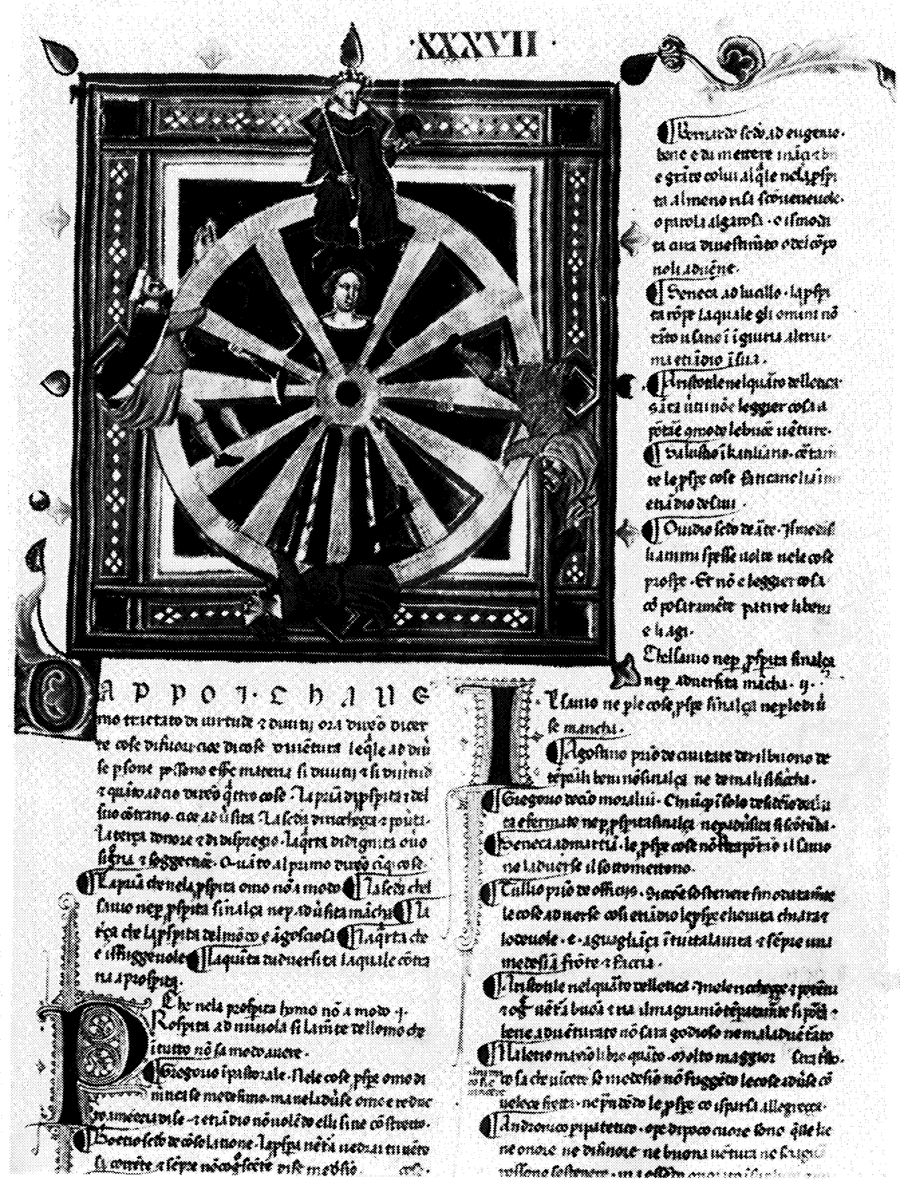
\includegraphics{include/html/images/322_1.png}

PLATE 1. \emph{Wheel of Fortune}. Codex miniature. Biblioteca Nazionale,
Florence, Italy. Courtesy of Alinari/Art Resource, New York.

\protect\hypertarget{20_ILLUSTRATIONS_FOLLOW_PAGE.xhtmlux5cux23id_3}{}{}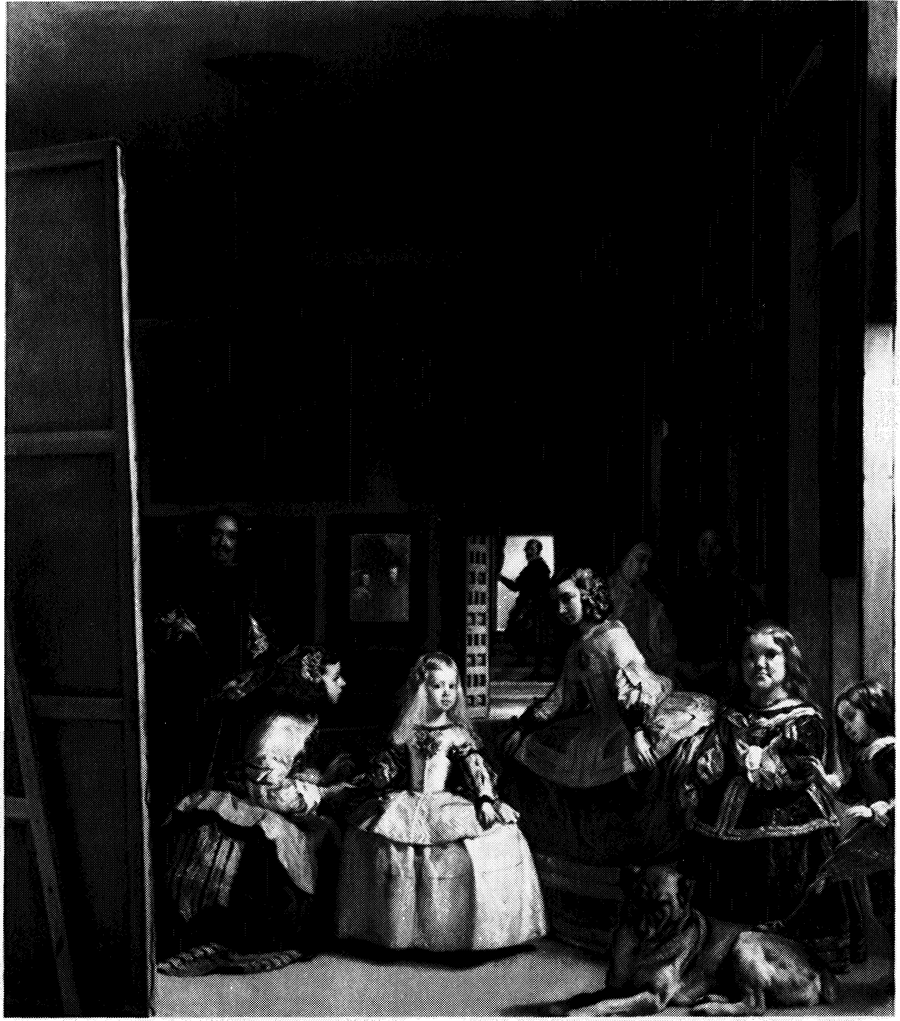
\includegraphics{include/html/images/323_1.png}

PLATE 2. Velazquez, Diego Rodriguez de Silva. \emph{The Maids of Honor}.
Prado, Madrid.

\protect\hypertarget{20_ILLUSTRATIONS_FOLLOW_PAGE.xhtmlux5cux23id_4}{}{}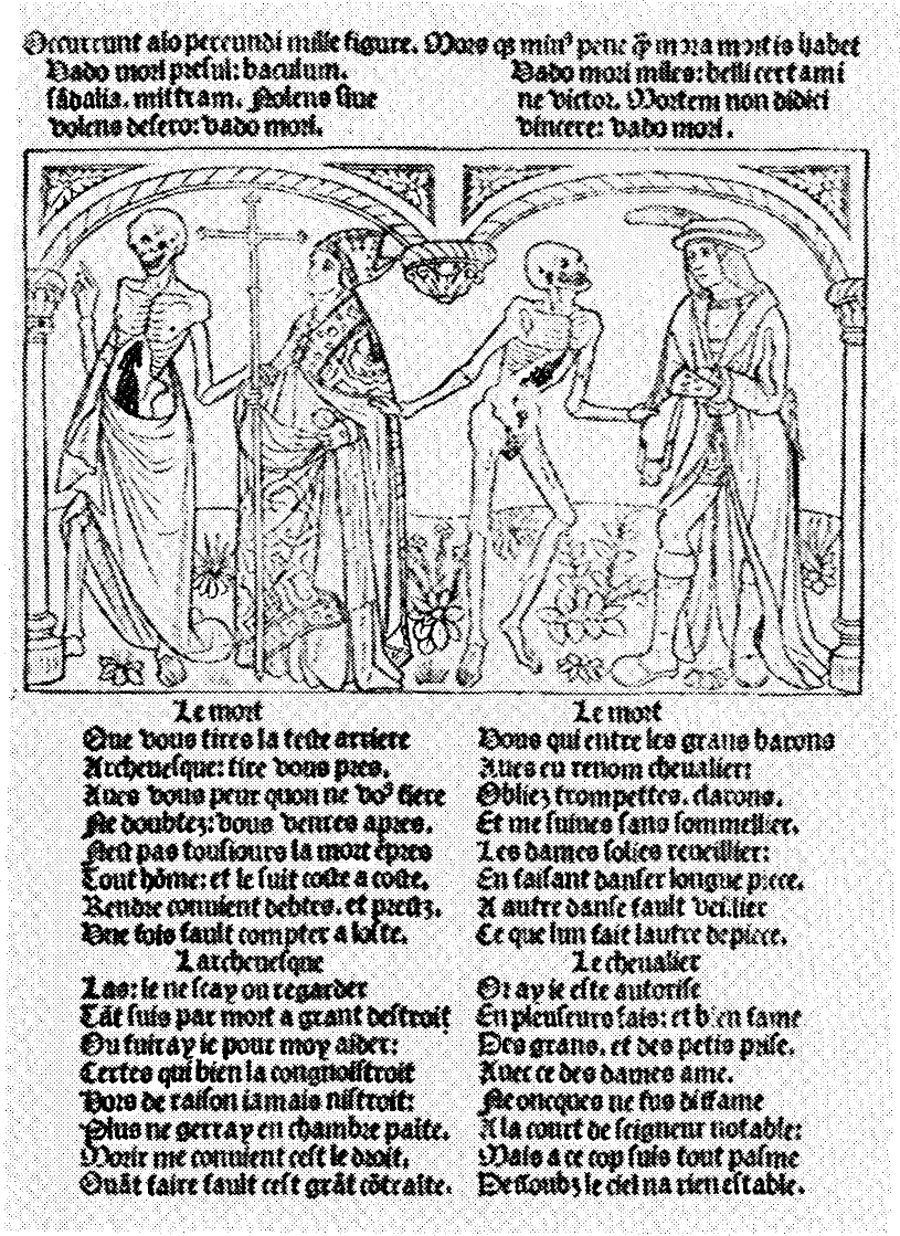
\includegraphics{include/html/images/324_1.png}

PLATE 3. Marchand, Guyot. \emph{Danse Macabre}. 1486. Bibliothèque
Nationale, Paris. Courtesy of Giraudon/Art Resource, New York.

\protect\hypertarget{20_ILLUSTRATIONS_FOLLOW_PAGE.xhtmlux5cux23id_2297}{}{}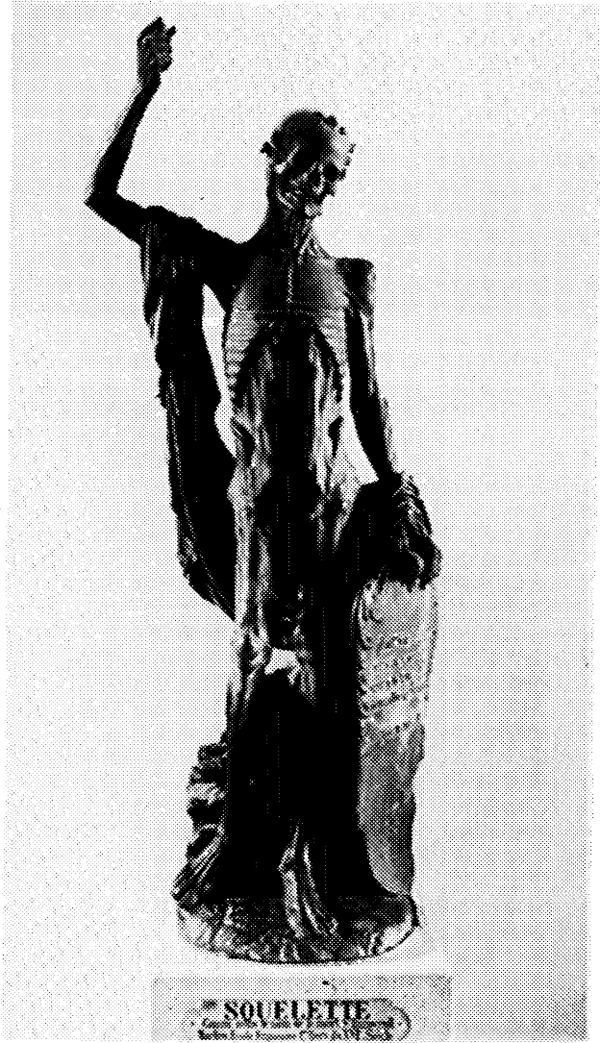
\includegraphics{include/html/images/324_2.png}

PLATE 4. French School. Figure of Death from the Cemetery of the
Innocents, Paris. 16th century. Louvre, Paris. Courtesy of Giraudon/Art
Resource, New York.

\protect\hypertarget{20_ILLUSTRATIONS_FOLLOW_PAGE.xhtmlux5cux23id_5}{}{}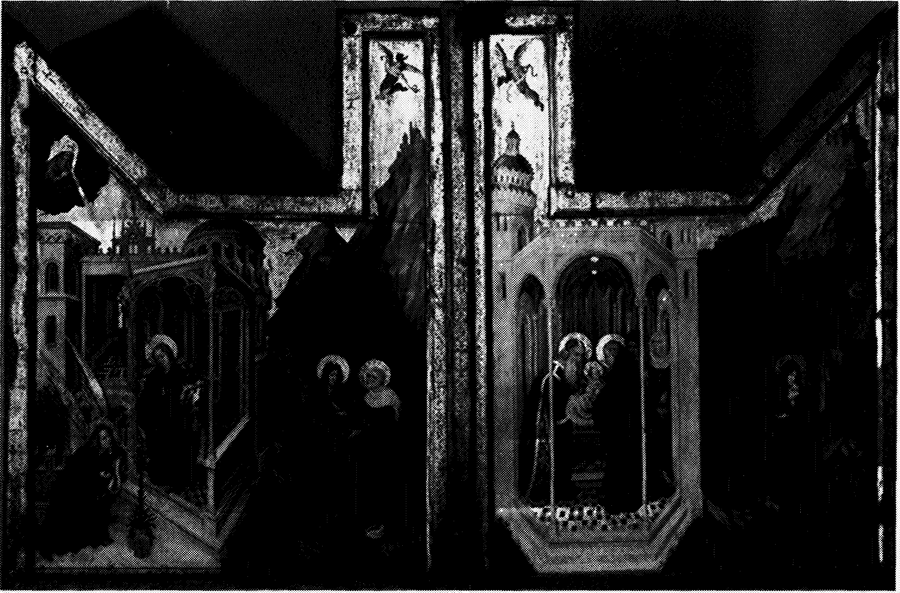
\includegraphics{include/html/images/325_1.png}

PLATE 5. Broederlam, Melchior. \emph{The Flight into Egypt}. Musée de
Beaux-Arts, Dijon.

\protect\hypertarget{20_ILLUSTRATIONS_FOLLOW_PAGE.xhtmlux5cux23id_6}{}{}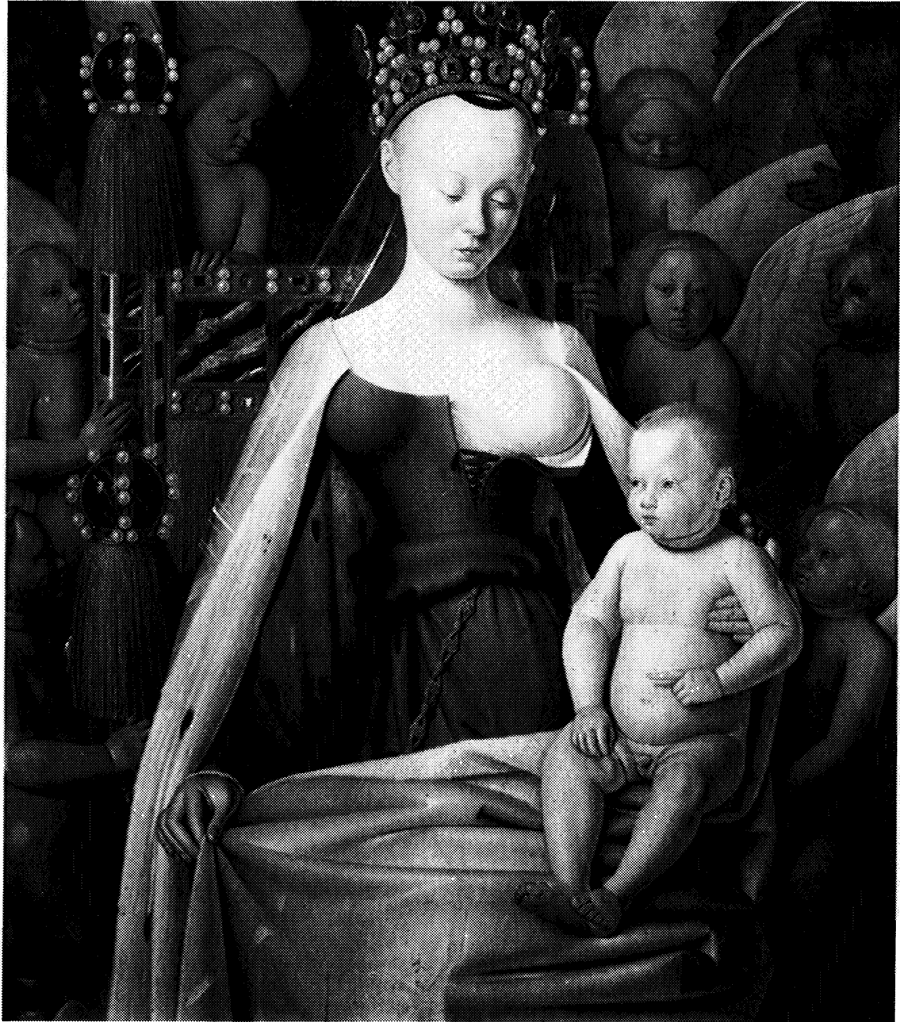
\includegraphics{include/html/images/326_1.png}

PLATE 6. Foucquet, Jean. \emph{Melun Madonna}. Koninklijk Museum,
Antwerp.

\protect\hypertarget{20_ILLUSTRATIONS_FOLLOW_PAGE.xhtmlux5cux23id_7}{}{}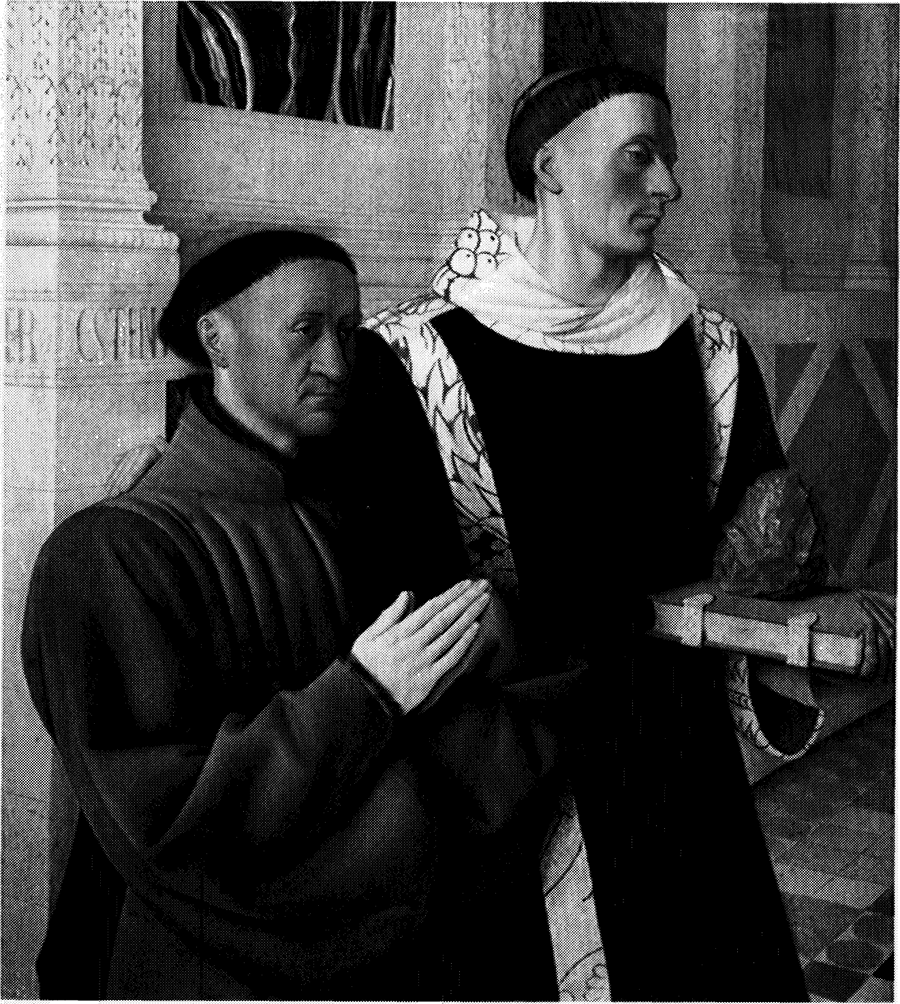
\includegraphics{include/html/images/327_1.png}

PLATE 7. Foucquet, Jean. \emph{Etienne Chevalier with St. Stephen}.
Gemaeldegalerie, Staatliche Museen, Berlin. Courtesy of Foto Marburg/Art
Resource, New York.

\protect\hypertarget{20_ILLUSTRATIONS_FOLLOW_PAGE.xhtmlux5cux23id_8}{}{}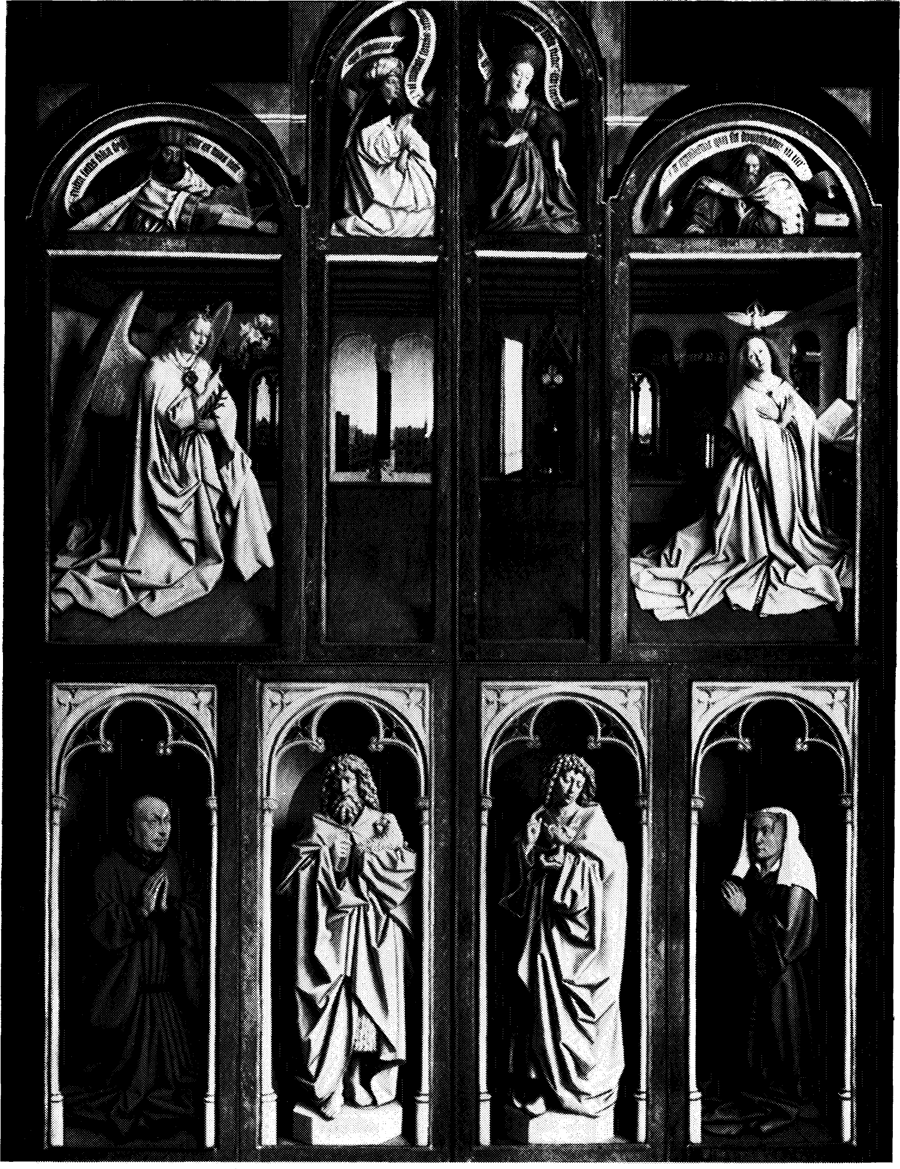
\includegraphics{include/html/images/328_1.png}

PLATE 8. Van Eyck, Jan. Ghent Altarpiece, closed. 1432. Cathedral St.
Bavo, Ghent. Courtesy of Giraudon/Art Resource, New York.

\protect\hypertarget{20_ILLUSTRATIONS_FOLLOW_PAGE.xhtmlux5cux23id_9}{}{}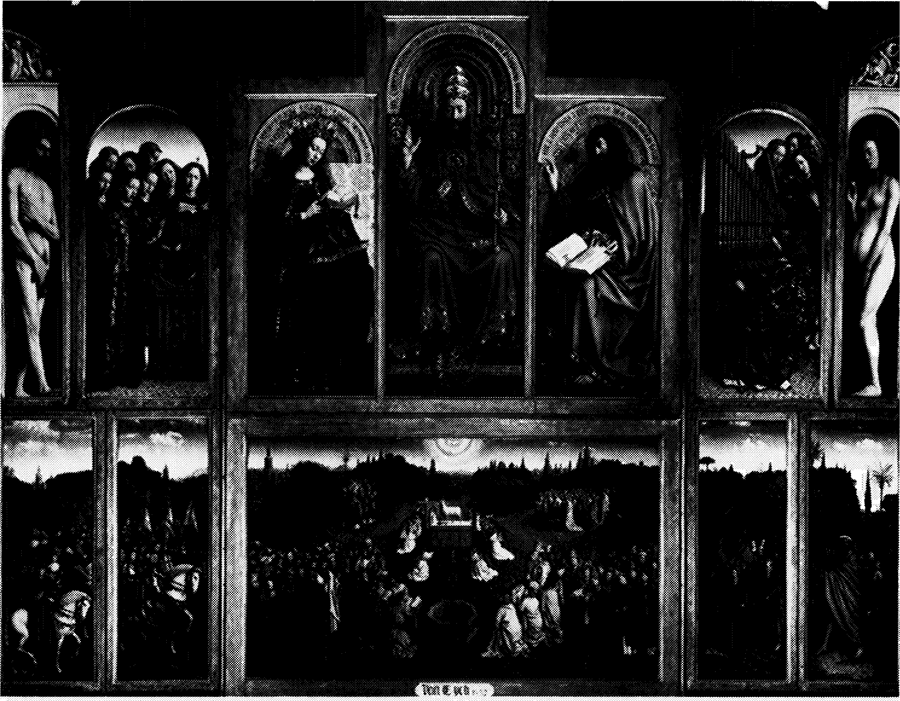
\includegraphics{include/html/images/329_1.png}

PLATE 9. Van Eyck, Jan. Ghent Altarpiece, open. 1432. Cathedral St.
Bavo, Ghent. Courtesy of Giraudon/Art Resource, New York.

\protect\hypertarget{20_ILLUSTRATIONS_FOLLOW_PAGE.xhtmlux5cux23id_10}{}{}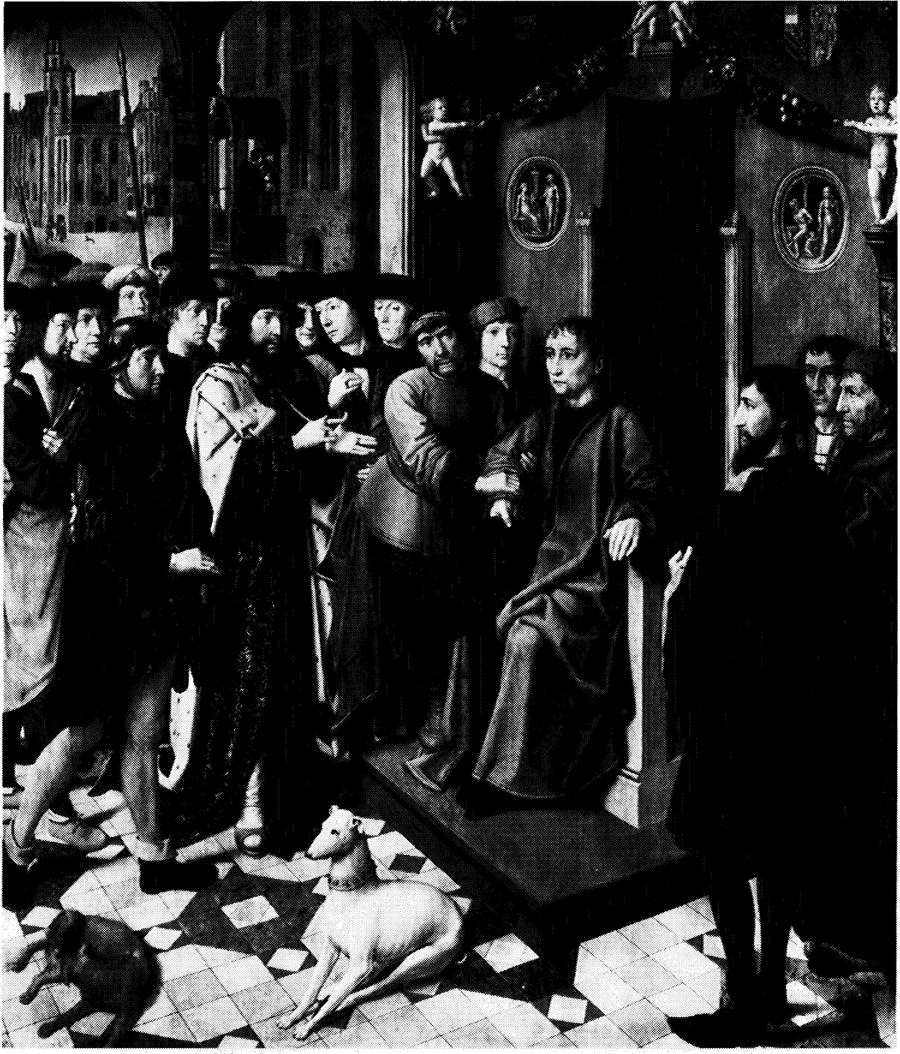
\includegraphics{include/html/images/330_1.png}

PLATE 10. David, Gerard. \emph{Judgement of Cambyses}. Municipal Museum,
Bruges. Courtesy of Alinari/Art Resource, New York.

\protect\hypertarget{20_ILLUSTRATIONS_FOLLOW_PAGE.xhtmlux5cux23id_11}{}{}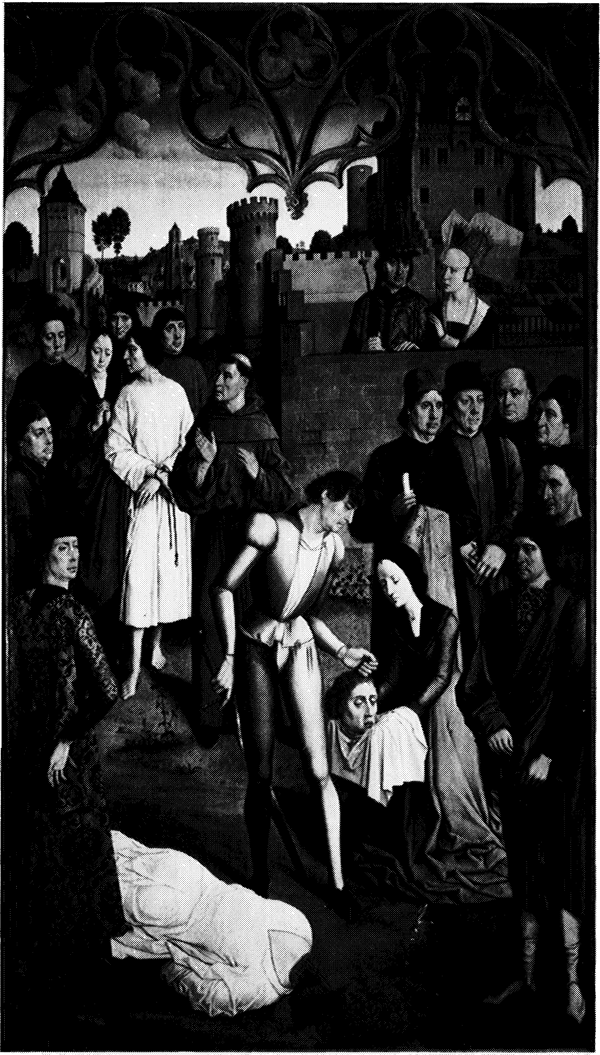
\includegraphics{include/html/images/331_1.png}

PLATE 11. Bouts, Dirk. \emph{Judgement of the Emperor Otto} (Scene 1).
Musée Royaux, Brussels.

\protect\hypertarget{20_ILLUSTRATIONS_FOLLOW_PAGE.xhtmlux5cux23id_12}{}{}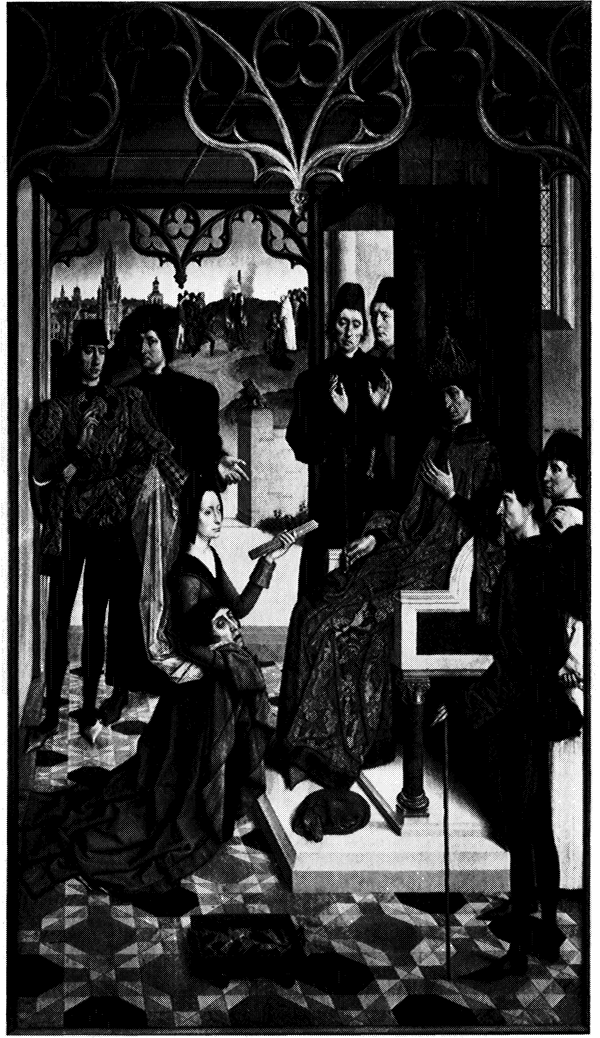
\includegraphics{include/html/images/332_1.png}

(Scene 2)

\protect\hypertarget{20_ILLUSTRATIONS_FOLLOW_PAGE.xhtmlux5cux23id_13}{}{}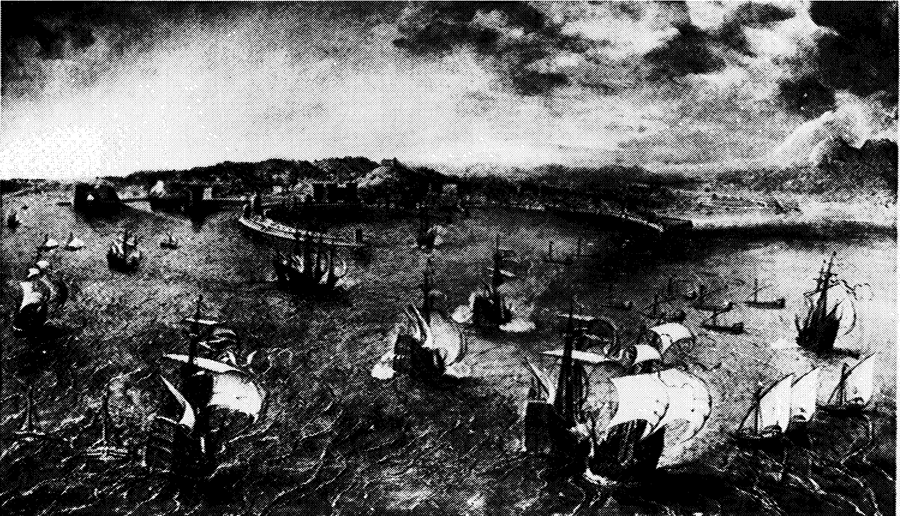
\includegraphics{include/html/images/333_1.png}

PLATE 12. Breughel, Pieter the Elder. The Old Port of Naples. Palazzo
Doria, Rome. Courtesy of Alinari/Art Resource, New York.

\protect\hypertarget{20_ILLUSTRATIONS_FOLLOW_PAGE.xhtmlux5cux23id_14}{}{}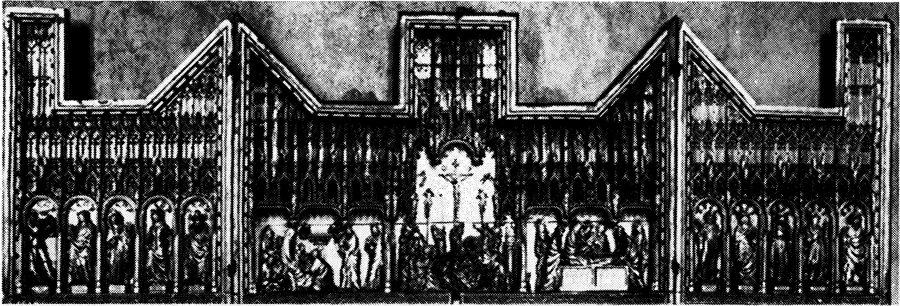
\includegraphics{include/html/images/334_1.png}

PLATE 13. Baerze, Jacques de. \emph{Retable of the Crucifixion}. Musée
des Beaux-Arts, Dijon.

\protect\hypertarget{20_ILLUSTRATIONS_FOLLOW_PAGE.xhtmlux5cux23id_2298}{}{}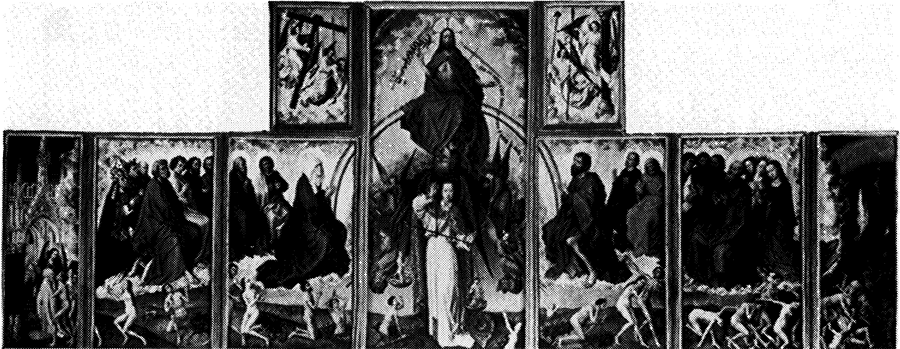
\includegraphics{include/html/images/334_2.png}

PLATE 14. Van der Weyden, Rogier. \emph{Last Judgement Altarpiece}
(open). Hotel-Dieu, Beaune, France. Courtesy of Giraudon/Art Resource,
New York.

\protect\hypertarget{20_ILLUSTRATIONS_FOLLOW_PAGE.xhtmlux5cux23id_15}{}{}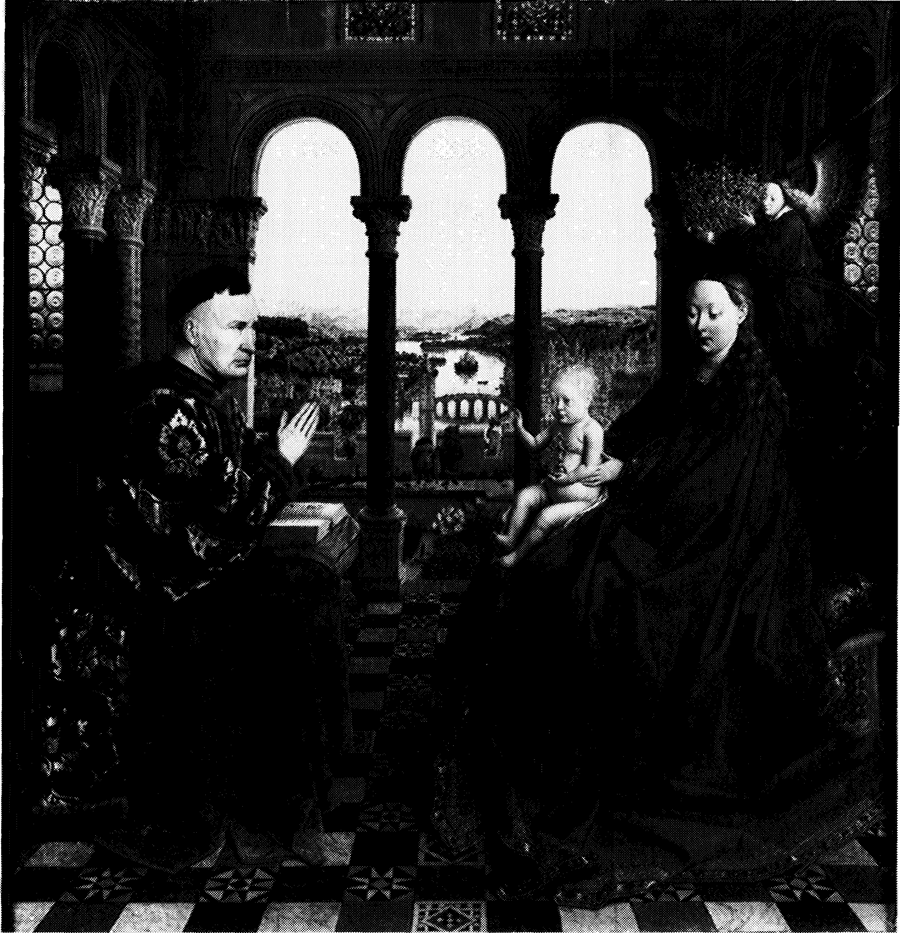
\includegraphics{include/html/images/335_1.png}

PLATE 15. Van Eyck Jan. \emph{Autun Altarpieoe}. Louvre, Paris. Cliché
des Musées Nationaux, Paris.

\protect\hypertarget{20_ILLUSTRATIONS_FOLLOW_PAGE.xhtmlux5cux23id_16}{}{}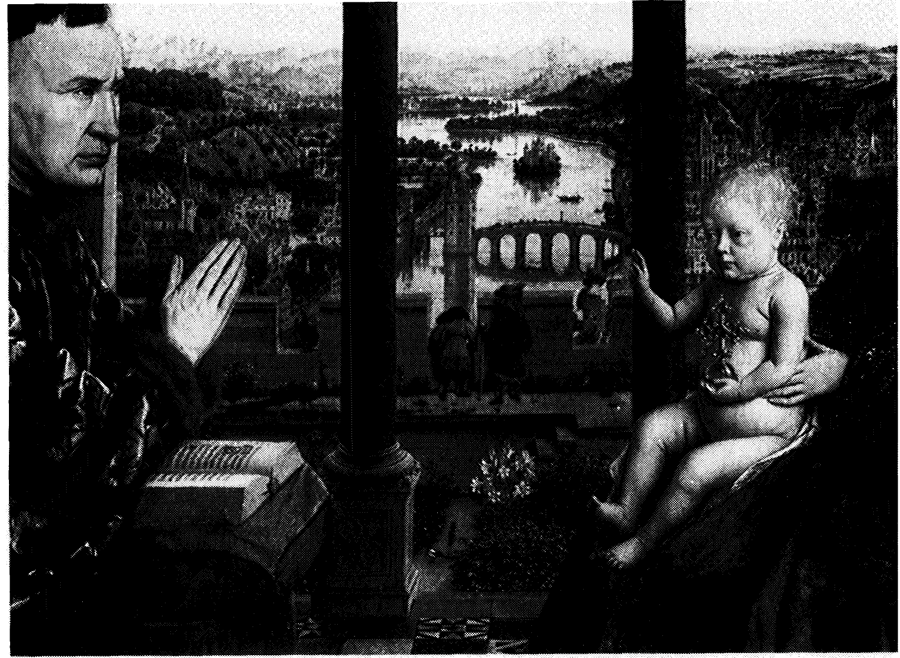
\includegraphics{include/html/images/336_1.png}

PLATE 16. Van Eyck, Jan. \emph{Autun Altarpiece}: detail of landscape in
background. Louvre, Paris. Cliché des Musées Nationaux, Paris.

\protect\hypertarget{20_ILLUSTRATIONS_FOLLOW_PAGE.xhtmlux5cux23id_17}{}{}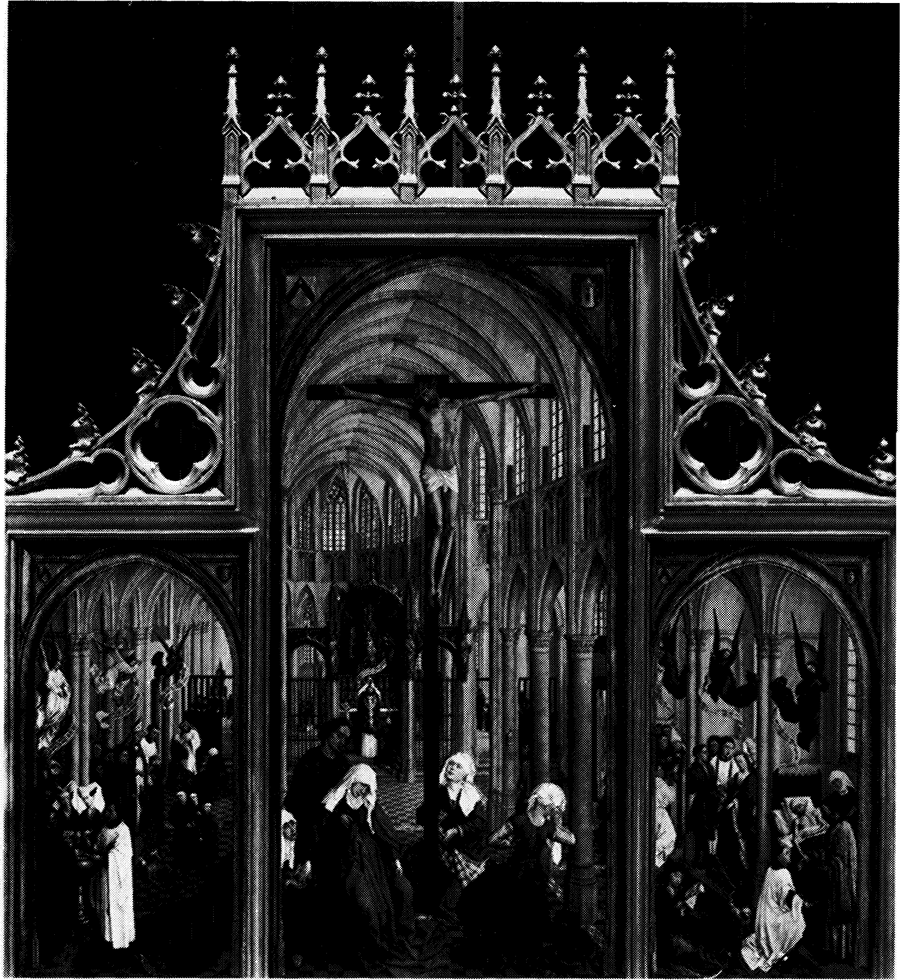
\includegraphics{include/html/images/337_1.png}

PLATE 17. Van der Weyden, Rogier. \emph{Altarpiece of the Seven
Sacraments}. Koninklijk Museum, Antwerp.

\protect\hypertarget{20_ILLUSTRATIONS_FOLLOW_PAGE.xhtmlux5cux23id_18}{}{}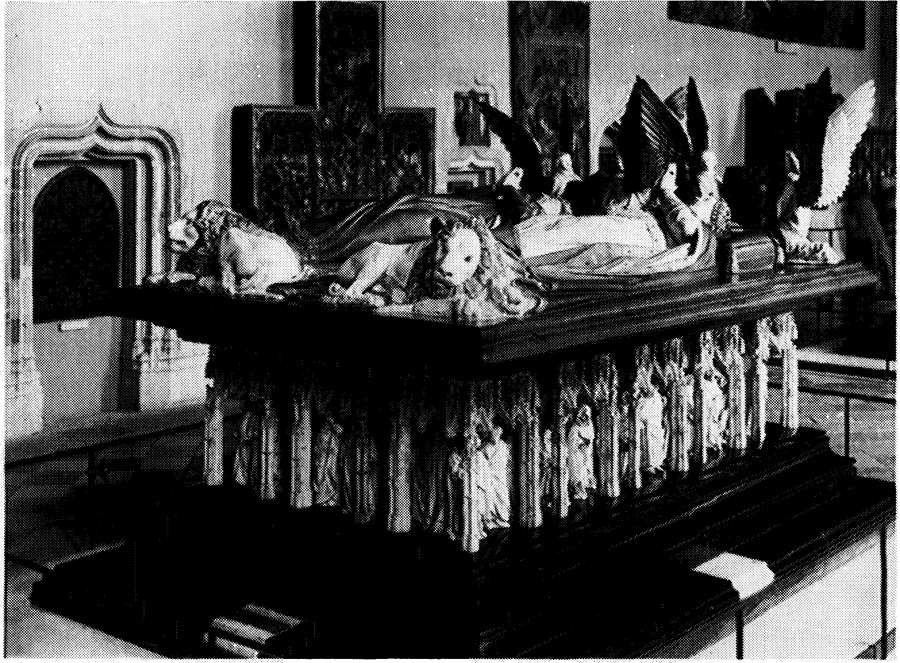
\includegraphics{include/html/images/338_1.png}

PLATE 18. Juan de la Huerta/Antoine le Moiturier. \emph{Tomb of John the
Fearless}. Musée des Beaux-Arts, Dijon.

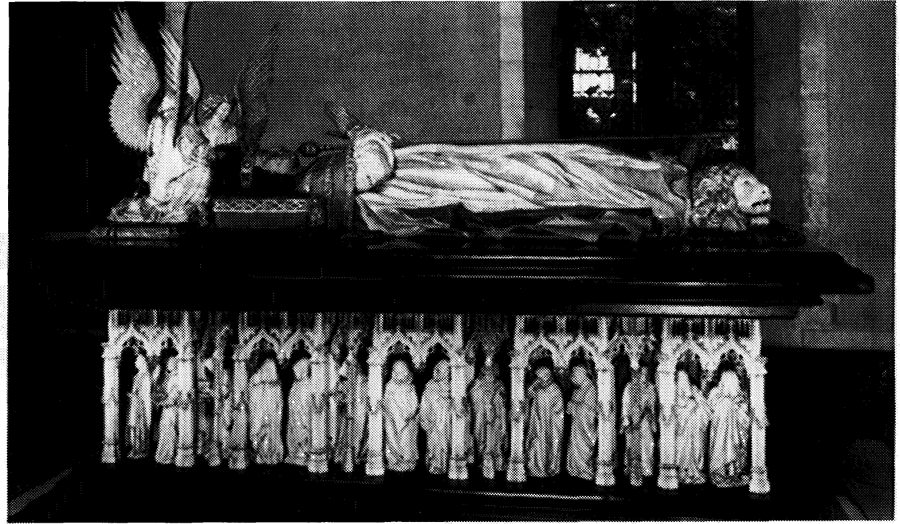
\includegraphics{include/html/images/338_2.png}

PLATE 19. Claus Sluter/Claus de Werve. \emph{Tomb of Philip the Bold}.
Musée de Beaux-Arts, Dijon.

\protect\hypertarget{20_ILLUSTRATIONS_FOLLOW_PAGE.xhtmlux5cux23id_19}{}{}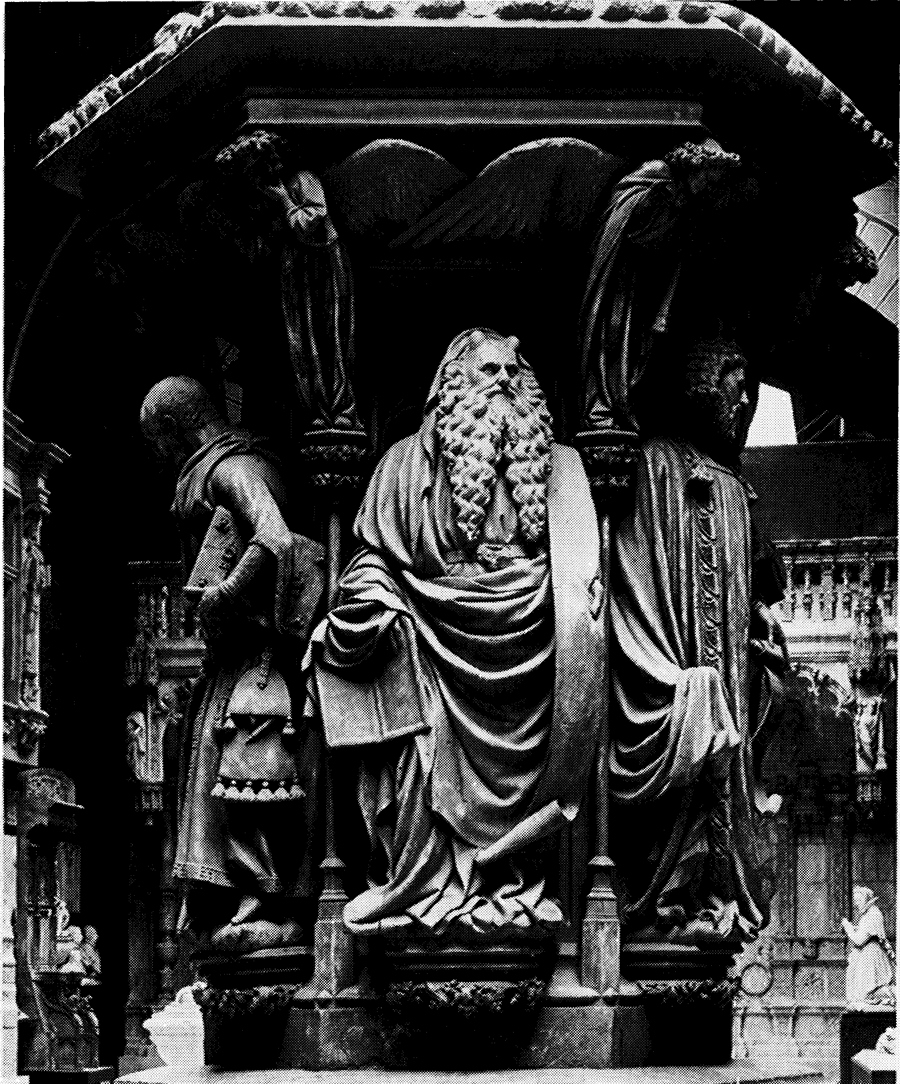
\includegraphics{include/html/images/339_1.png}

PLATE 20. Sluter, Claus. Moses from \emph{The Well of Moses}.
1395--1404. Chartreuse de Champmol, Dijon. Courtesy of Giraudon/Art
Resource, New York.

\protect\hypertarget{20_ILLUSTRATIONS_FOLLOW_PAGE.xhtmlux5cux23id_20}{}{}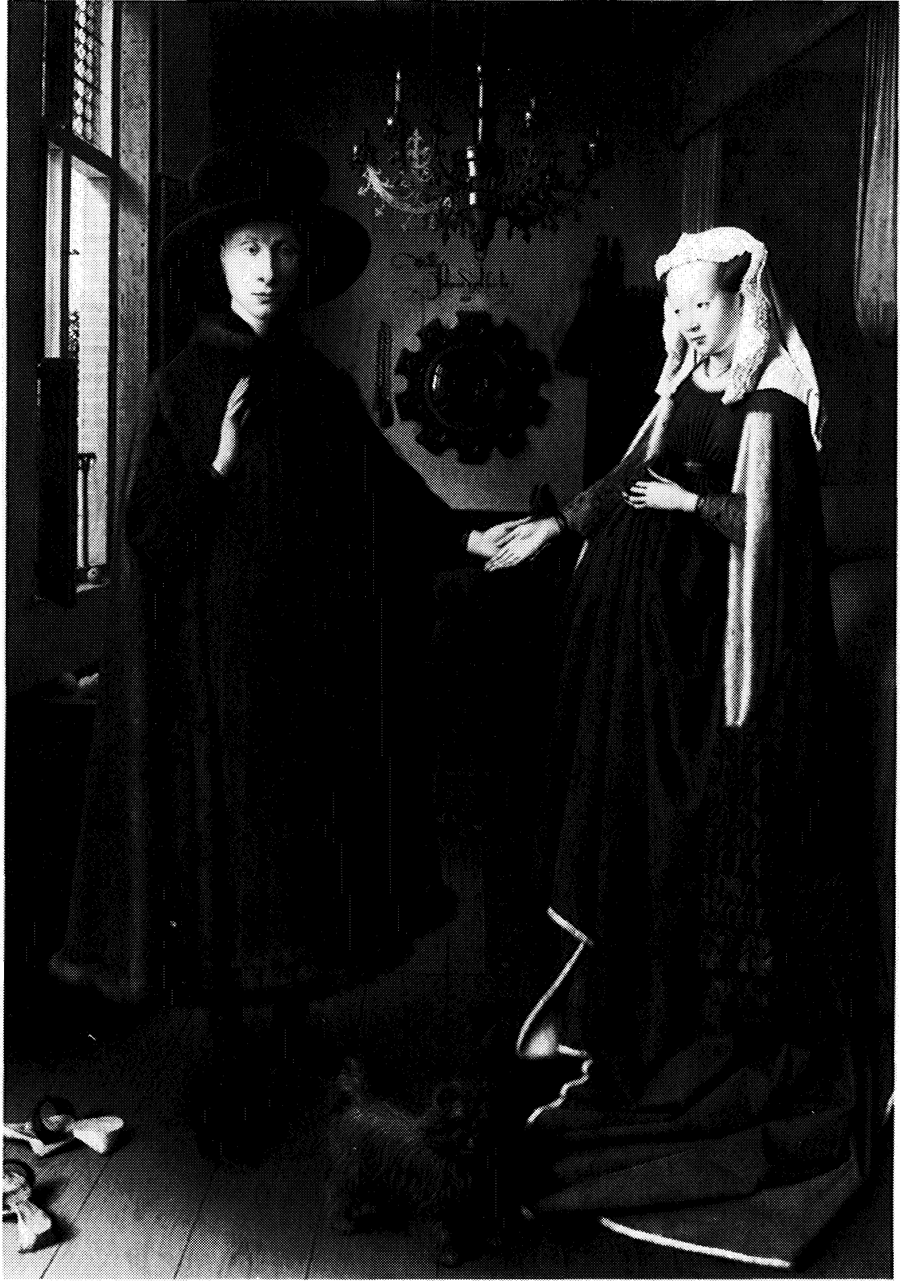
\includegraphics{include/html/images/340_1.png}

PLATE 21. Van Eyck, Jan. \emph{Wedding Portrait (Giovanni Amolfini and
Cenami Arnolfini)}. Reproduced by courtesy of the Trustees, The National
Gallery, London.

\protect\hypertarget{20_ILLUSTRATIONS_FOLLOW_PAGE.xhtmlux5cux23id_21}{}{}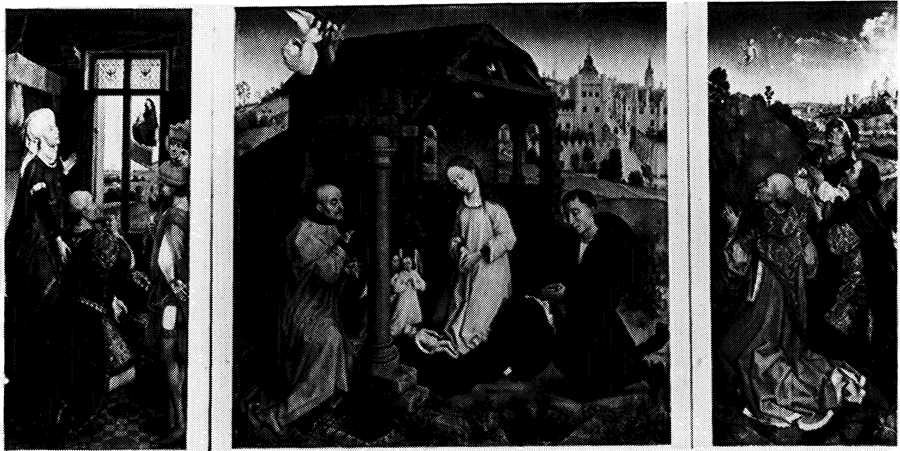
\includegraphics{include/html/images/341_1.png}

PLATE 22. Van der Weyden, Rogier. \emph{Bladelin Altarpiece}.
Gemaeldegalerie, Staatliche Museen, Berlin. Courtesy of Giraudon/Art
Resource, New York.

\protect\hypertarget{20_ILLUSTRATIONS_FOLLOW_PAGE.xhtmlux5cux23id_22}{}{}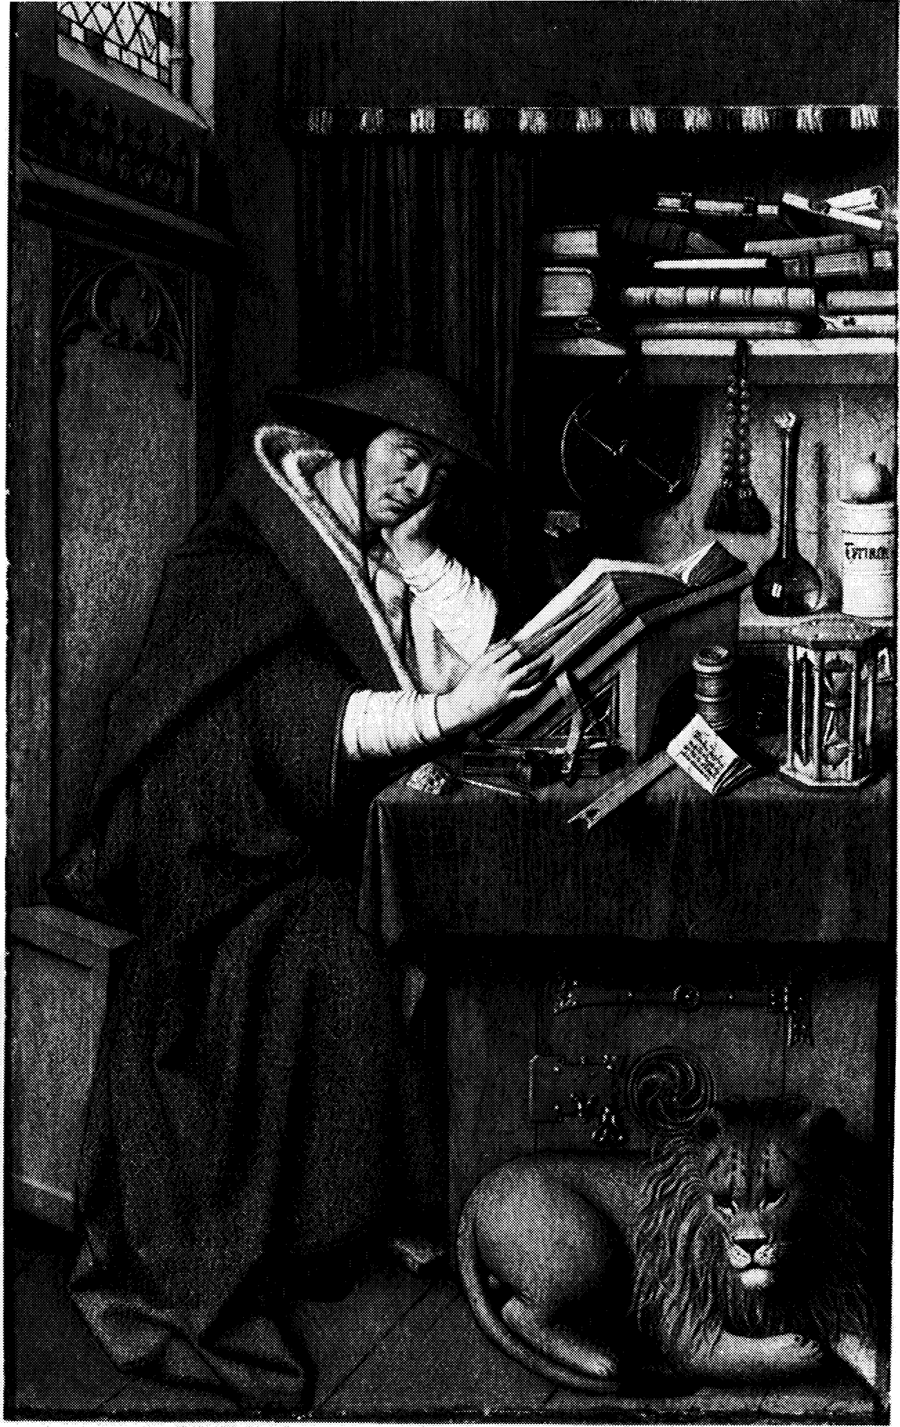
\includegraphics{include/html/images/342_1.png}

PLATE 23. Van Eyck, Jan. \emph{St. Jerome in His Study}. c. 1435. Oil on
linen paper on oak, 20.6 cm. x 13.3 cm. Accession no. 25.4. Photograph
©The Detroit Institute of Arts, 1995. City of Detroit Purchase.

\protect\hypertarget{20_ILLUSTRATIONS_FOLLOW_PAGE.xhtmlux5cux23id_23}{}{}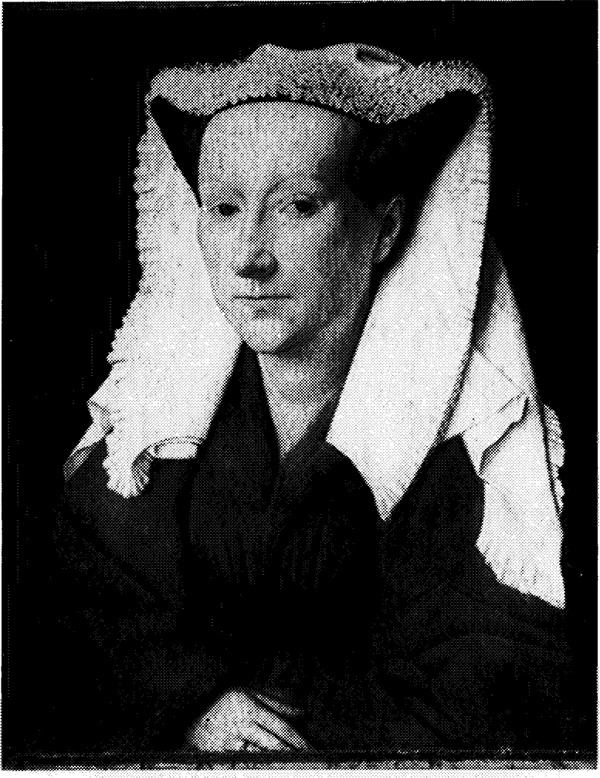
\includegraphics{include/html/images/343_1.png}

PLATE 24. Van Eyck, Jan. \emph{Margaretha van Eyck}. Municipal Museum,
Bruges. Courtesy of Foto Marburg/Art Resource, New York.

\protect\hypertarget{20_ILLUSTRATIONS_FOLLOW_PAGE.xhtmlux5cux23id_2299}{}{}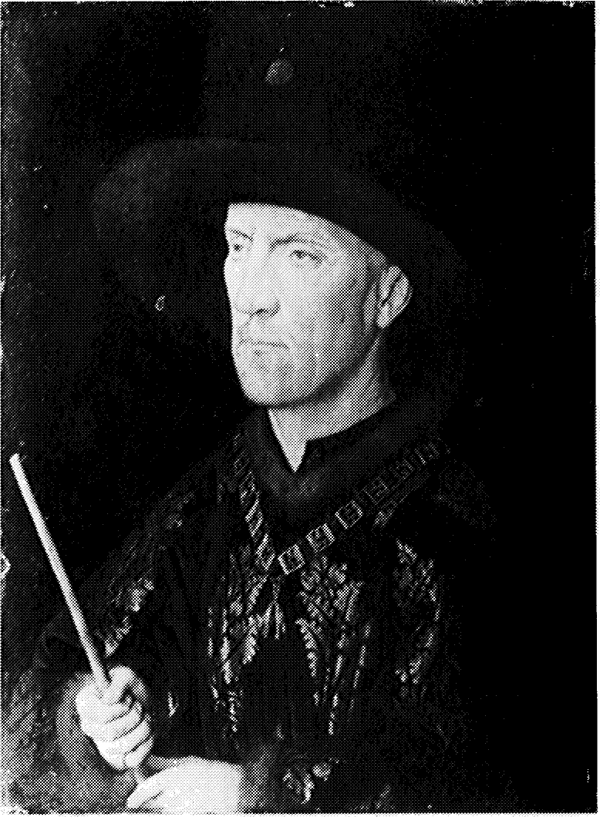
\includegraphics{include/html/images/343_2.png}

PLATE 25. Van Eyck, Jan. \emph{Baudoin de Lannoy}. Gemaeldegalerie,
Staatliche Museen, Berlin. Courtesy of Foto Marburg/Art Resource, New
York.

\protect\hypertarget{20_ILLUSTRATIONS_FOLLOW_PAGE.xhtmlux5cux23id_24}{}{}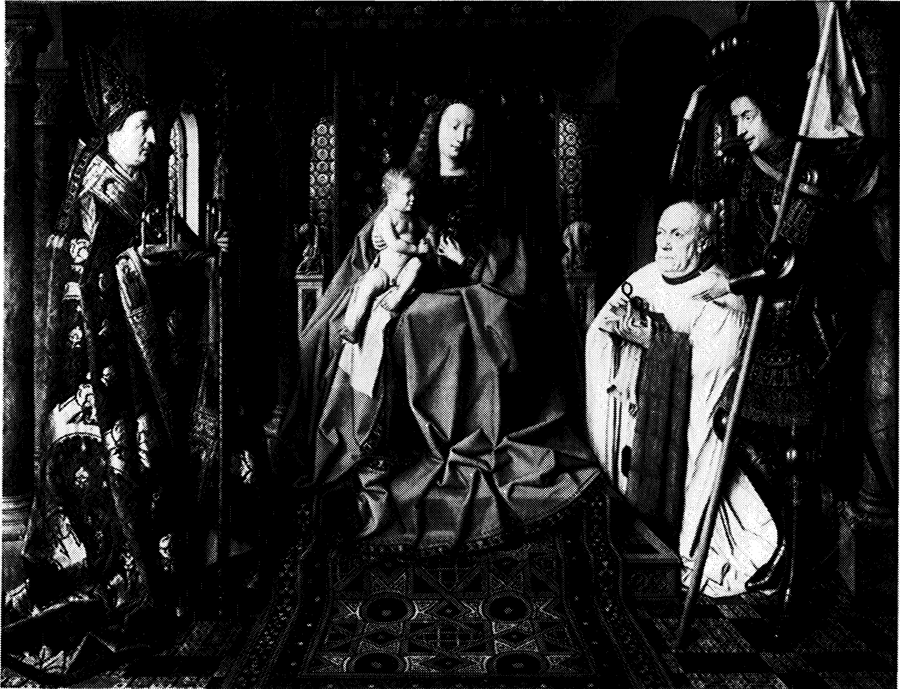
\includegraphics{include/html/images/344_1.png}

PLATE 26. Van Eyck, Jan. \emph{Madonna of Canon van der Paele}.
Municipal Museum, Bruges. Foto Marburg/Art Resource, New York.

\protect\hypertarget{20_ILLUSTRATIONS_FOLLOW_PAGE.xhtmlux5cux23id_25}{}{}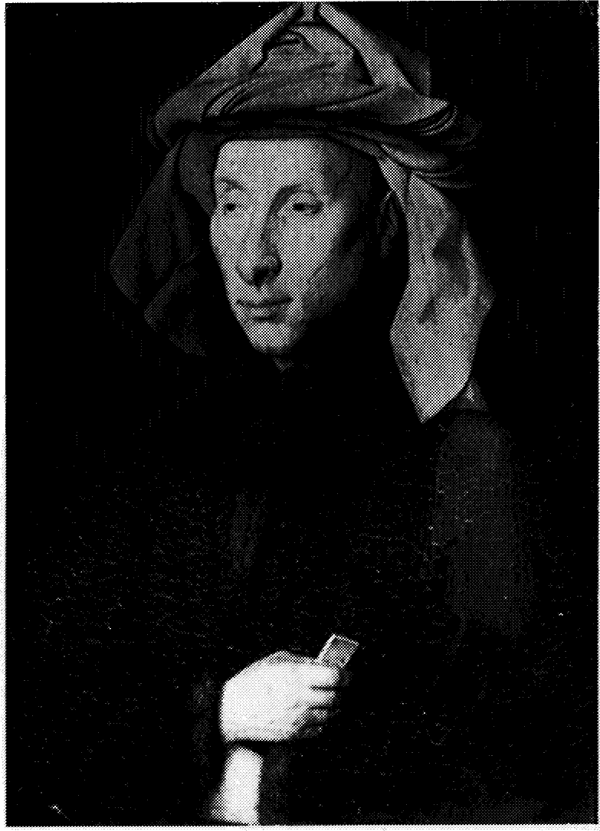
\includegraphics{include/html/images/345_1.png}

PLATE 27. Van Eyck, Jan. \emph{Giovanni Arnolfini}. Gemaeldegalerie,
Staatlich Museen, Berlin. Courtesy of Foto Marburg/Art Resource, New
York.

\protect\hypertarget{20_ILLUSTRATIONS_FOLLOW_PAGE.xhtmlux5cux23id_2300}{}{}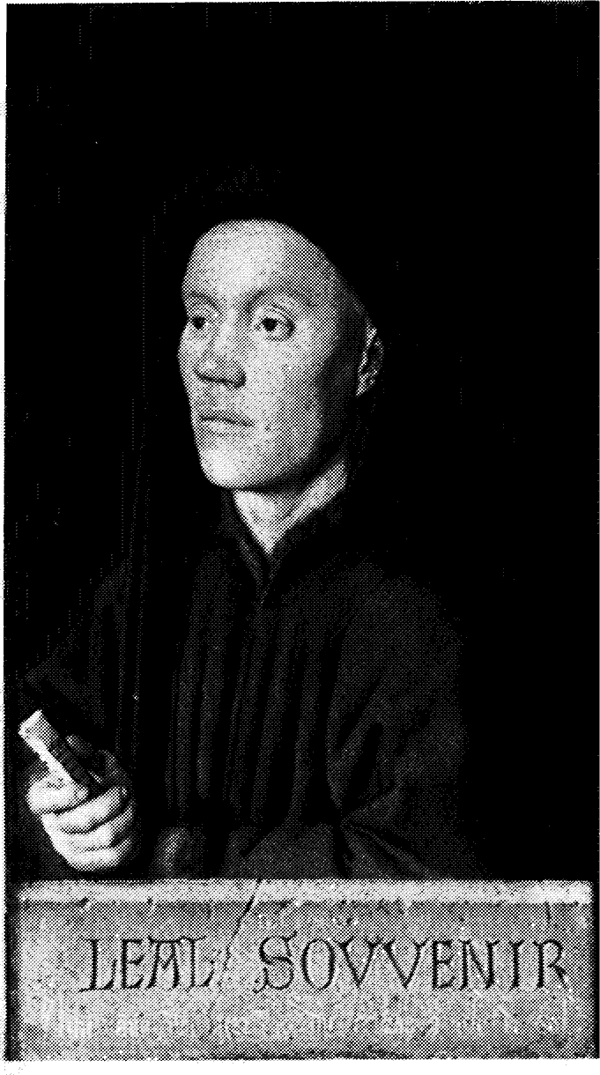
\includegraphics{include/html/images/345_2.png}

PLATE 28. Van Eyck, Jan. \emph{Leal Souvenier}. Reproduced by courtesy
of the Trustees, National Gallery, London.

\protect\hypertarget{20_ILLUSTRATIONS_FOLLOW_PAGE.xhtmlux5cux23id_26}{}{}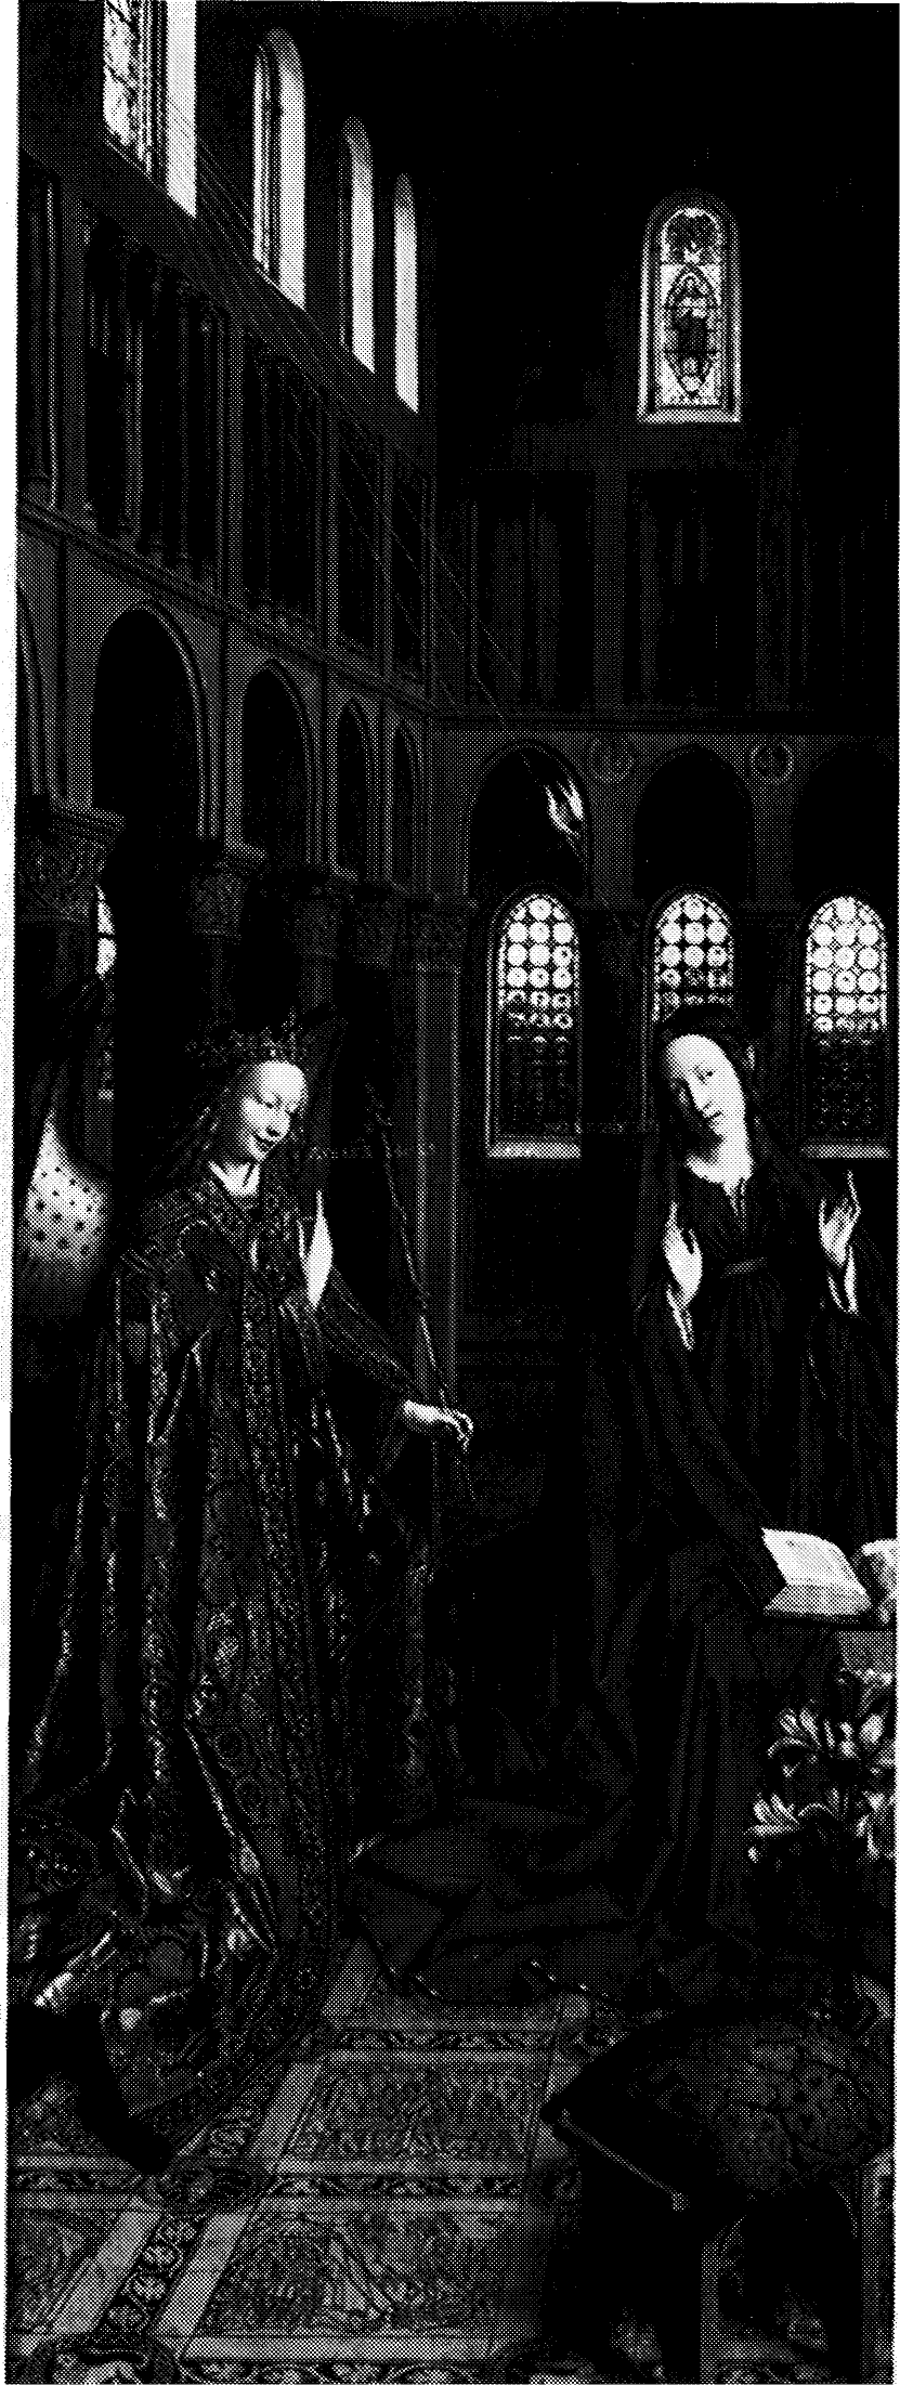
\includegraphics{include/html/images/346_1.png}

PLATE 29 (opposite). Van Eyck, Jan. \emph{Annunciation}. Andrew W.
Mellon Collection, © 1994 Board of Trustees, National Gallery of Art,
Washington, D.C.

\protect\hypertarget{20_ILLUSTRATIONS_FOLLOW_PAGE.xhtmlux5cux23id_27}{}{}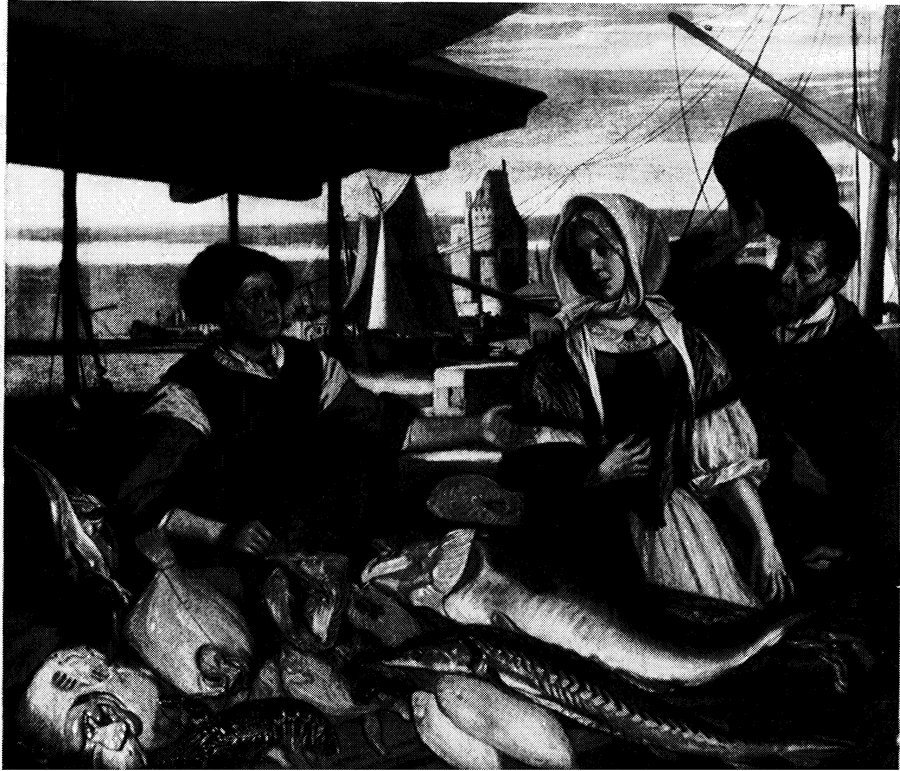
\includegraphics{include/html/images/347_1.png}

PLATE 30. De Witte, Emmanuel. \emph{The Fishmonger's Stall}. Courtesy of
Museum Boymans-van Beuningen, Rotterdam.

\protect\hypertarget{20_ILLUSTRATIONS_FOLLOW_PAGE.xhtmlux5cux23id_28}{}{}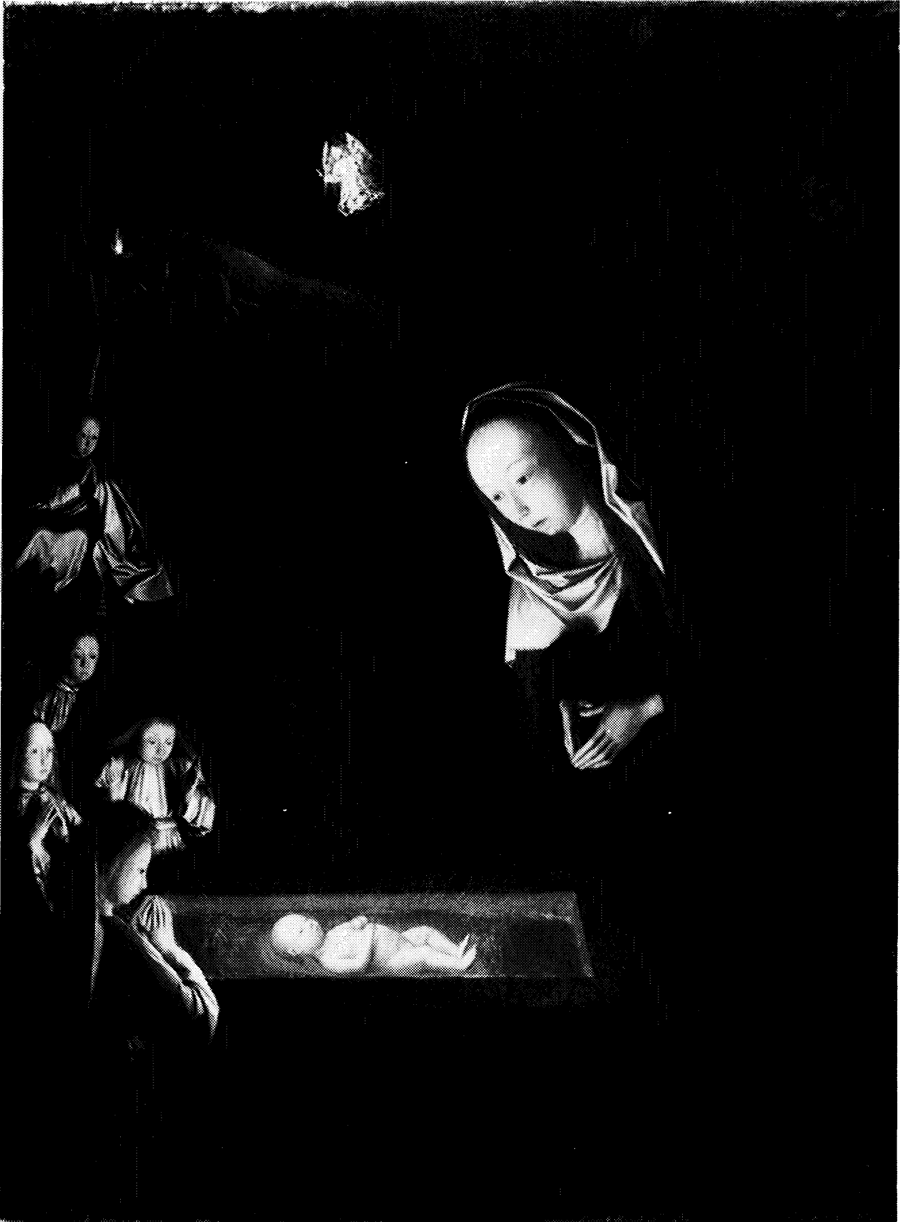
\includegraphics{include/html/images/348_1.png}

PLATE 31. Sint Jans, Geertgen tot. \emph{Nativity}. Reproduced by
courtesy of the Trustees, The National Gallery, London.

\protect\hypertarget{20_ILLUSTRATIONS_FOLLOW_PAGE.xhtmlux5cux23id_29}{}{}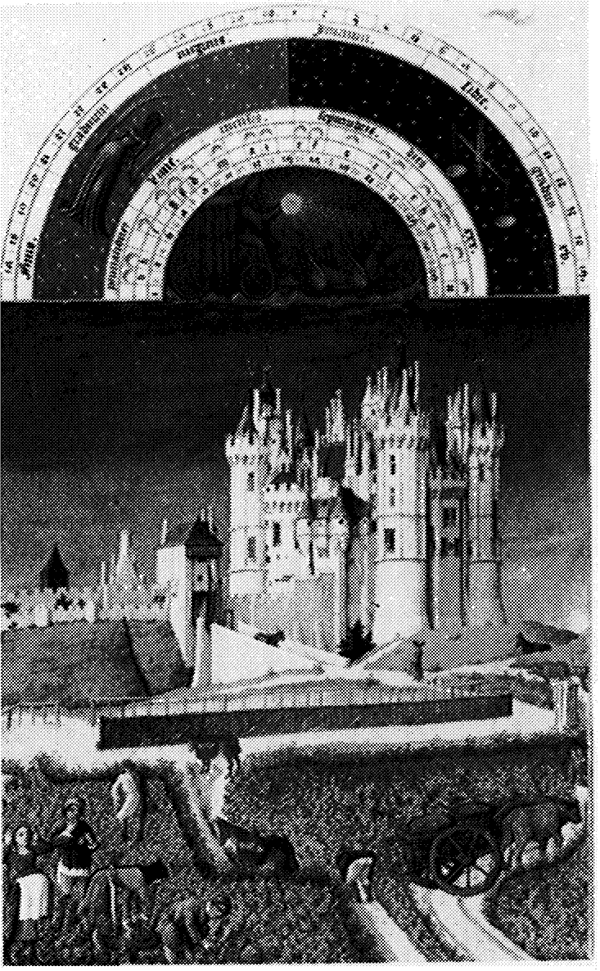
\includegraphics{include/html/images/349_1.png}

PLATE 32. Limburg Brothers. \emph{September (Grape Harvest)}. Calendar
page from the manuscript \emph{Très Riches Heures du Duc de Berry}.
Musée Conde, Chantilly. Courtesy of Giraudon/Art Resource, New York.

\protect\hypertarget{20_ILLUSTRATIONS_FOLLOW_PAGE.xhtmlux5cux23id_2301}{}{}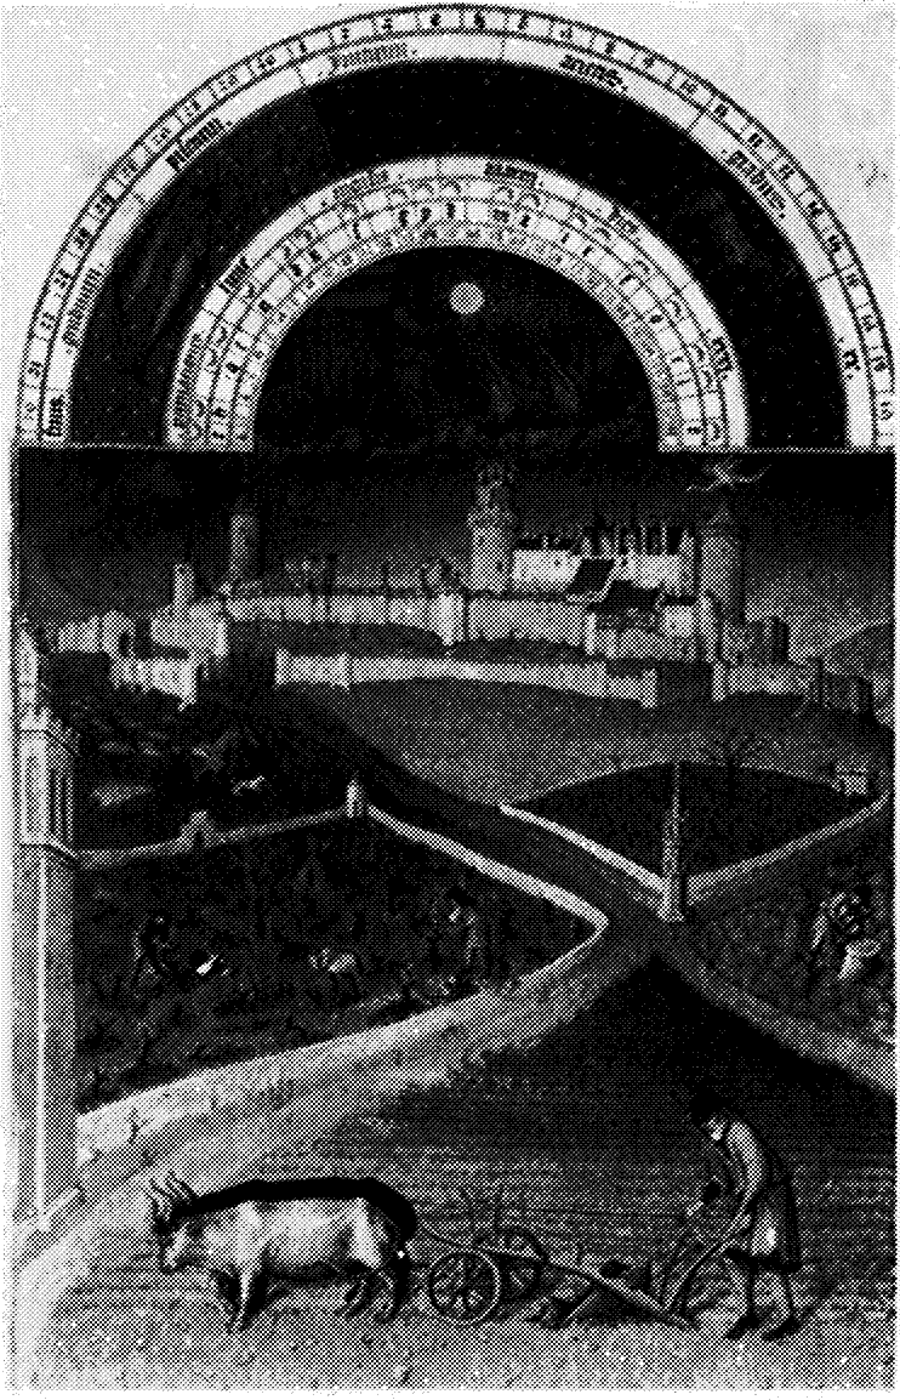
\includegraphics{include/html/images/349_2.png}

PLATE 33. Limburg Brothers. \emph{March}. Calendar page from \emph{Très
Riches Heures du Duc de Berry}. Musée Conde, Chantilly. Courtesy of
Giraudon/Art Resource, New York.

\protect\hypertarget{20_ILLUSTRATIONS_FOLLOW_PAGE.xhtmlux5cux23id_30}{}{}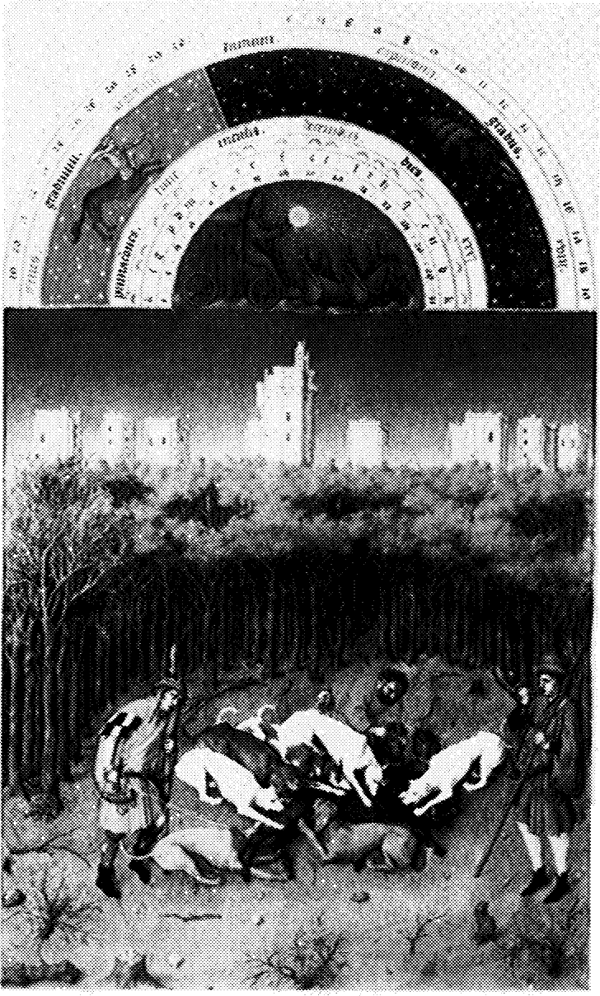
\includegraphics{include/html/images/350_1.png}

PLATE 34. Limburg Brothers. \emph{December}. Calendar page from
\emph{Très Riches Heures du Duc de Berry}. Musée Conde, Chantilly.
Courtesy of Giraudon/Art Resource, New York.

\protect\hypertarget{20_ILLUSTRATIONS_FOLLOW_PAGE.xhtmlux5cux23id_2302}{}{}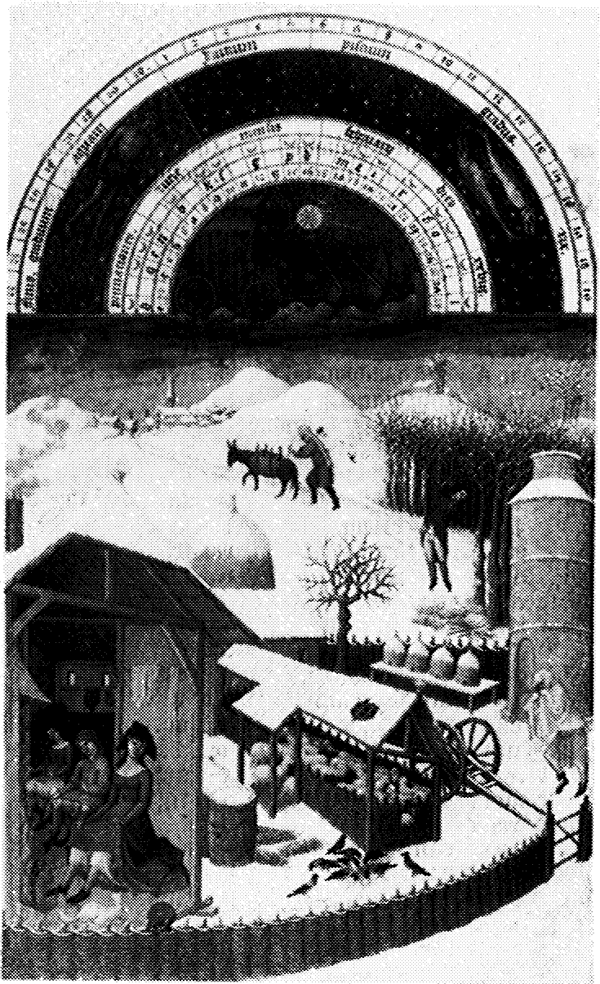
\includegraphics{include/html/images/350_2.png}

PLATE 35. Limburg Brothers. \emph{February}. Calendar page from
\emph{Très Riches Heures du Duc de Berry}. Musée Conde, Chantilly.
Courtesy of Giraudon/Art Resource, New York.

\protect\hypertarget{20_ILLUSTRATIONS_FOLLOW_PAGE.xhtmlux5cux23id_31}{}{}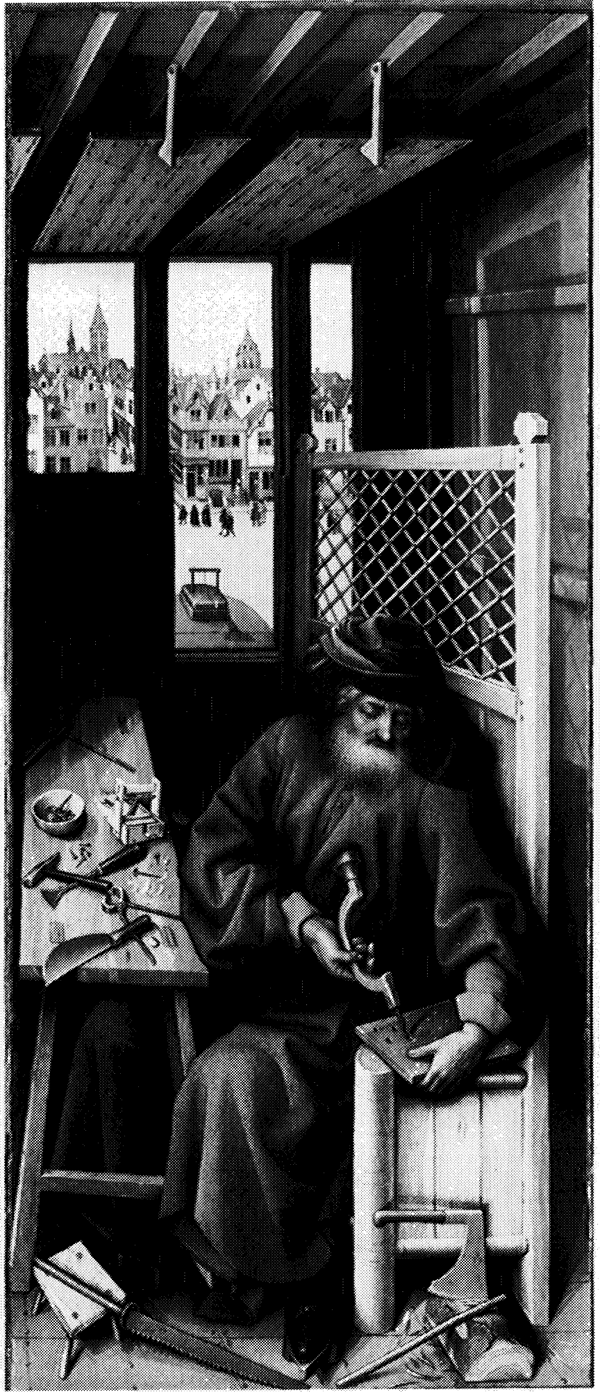
\includegraphics{include/html/images/351_1.png}

PLATE 36. Campin, Robert (Master of Flémalle). \emph{Annunciation}
(right panel). All rights reserved. The Metropolitan Museum of Art.

\protect\hypertarget{20_ILLUSTRATIONS_FOLLOW_PAGE.xhtmlux5cux23id_32}{}{}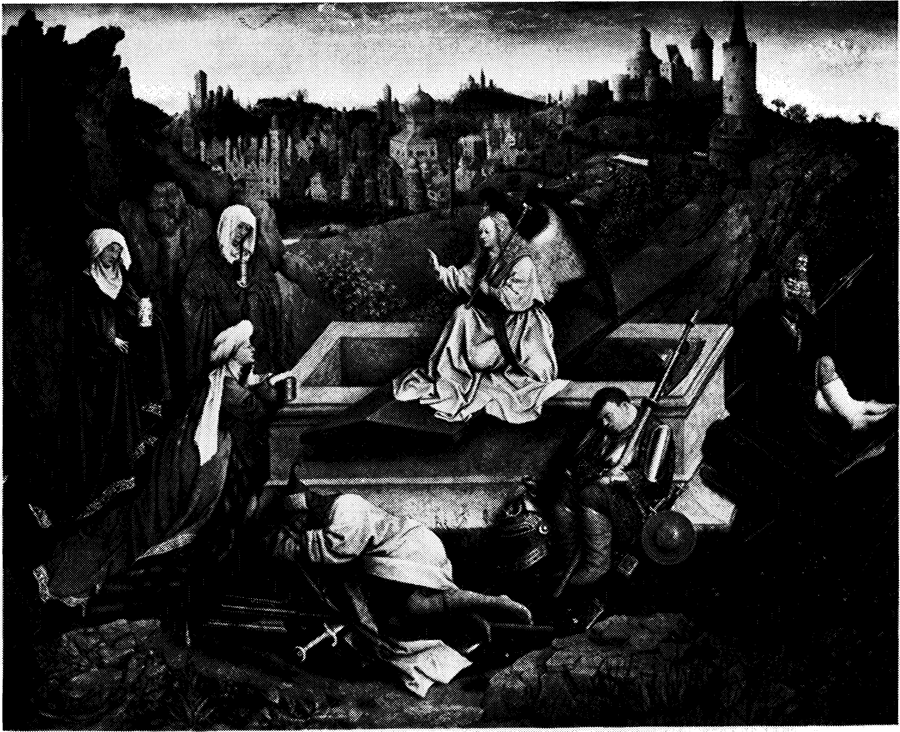
\includegraphics{include/html/images/352_1.png}

PLATE 37. Van Eyck, Hubert and Jan. \emph{The Three Marys at the Open
Sepulchre}. Museum Boymans-van Beuningen, Rotterdam.

\protect\hypertarget{20_ILLUSTRATIONS_FOLLOW_PAGE.xhtmlux5cux23id_33}{}{}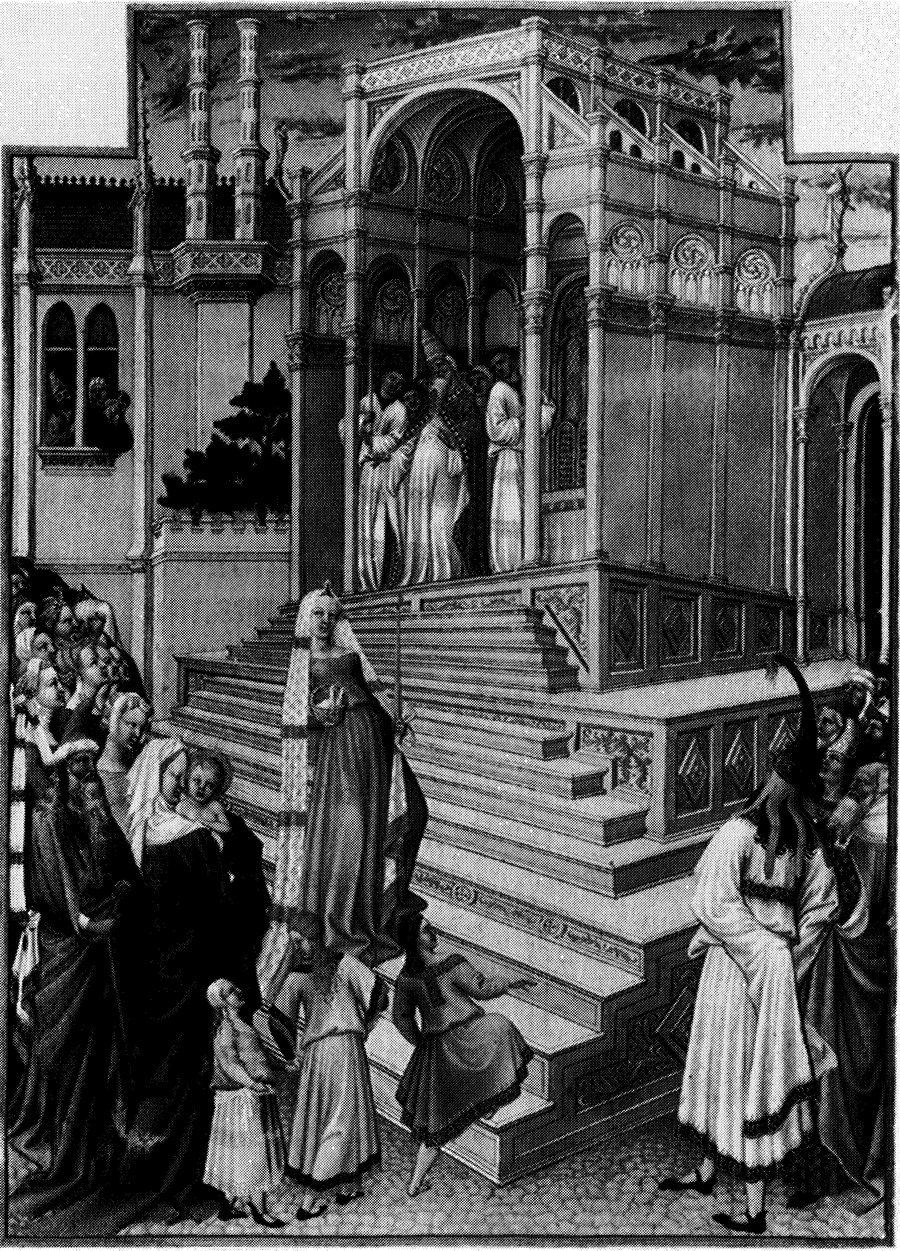
\includegraphics{include/html/images/353_1.png}

PLATE 38. Limburg Brothers. \emph{Purification}. From \emph{Très Riches
Heures du Duc de Berry}. Musée Conde, Chantilly. Courtesy of
Giraudon/Art Resource, New York.

\protect\hypertarget{20_ILLUSTRATIONS_FOLLOW_PAGE.xhtmlux5cux23id_34}{}{}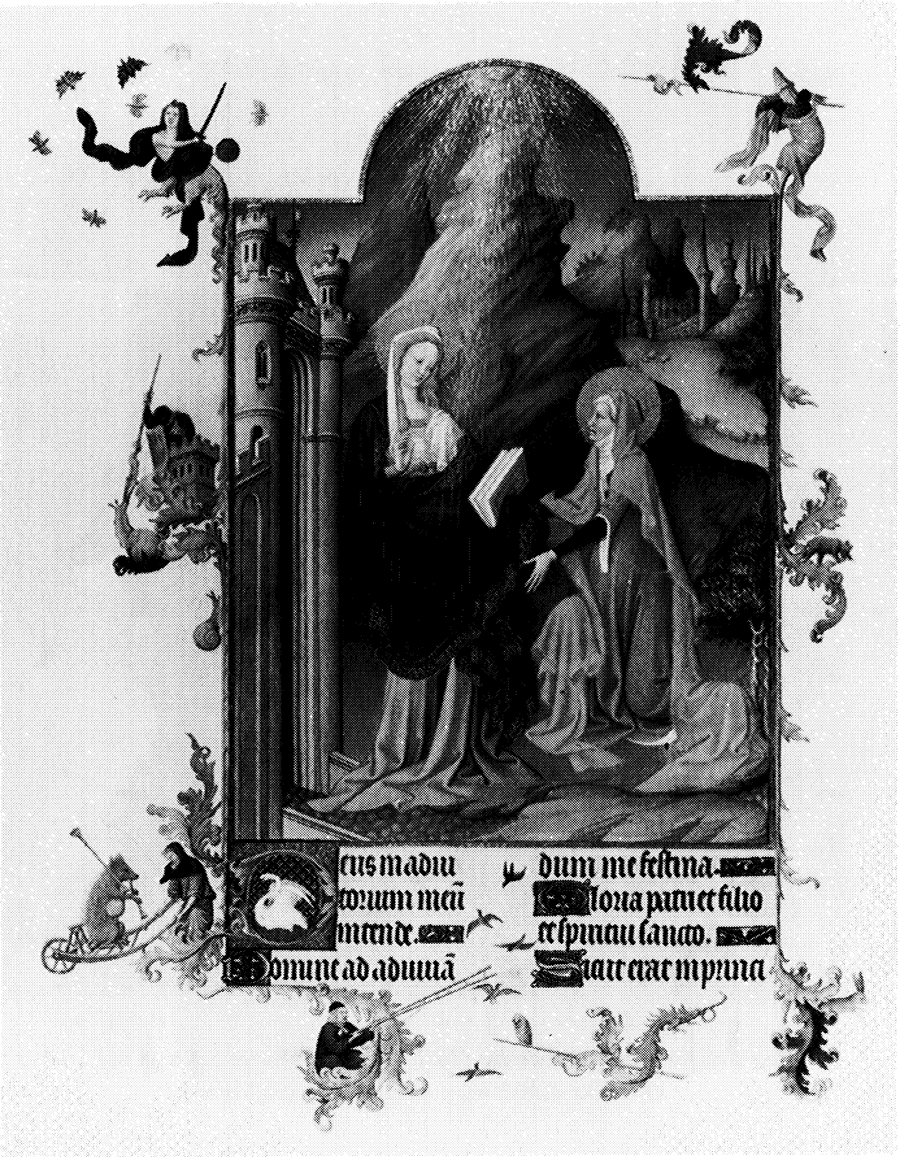
\includegraphics{include/html/images/354_1.png}

PLATE 39. Limburg Brothers. \emph{Visitation}. From \emph{Très Riches
Heures du Duc de Berry}. Musée Conde, Chantilly. Courtesy of
Giraudon/Art Resource, New York.

\protect\hypertarget{20_ILLUSTRATIONS_FOLLOW_PAGE.xhtmlux5cux23id_35}{}{}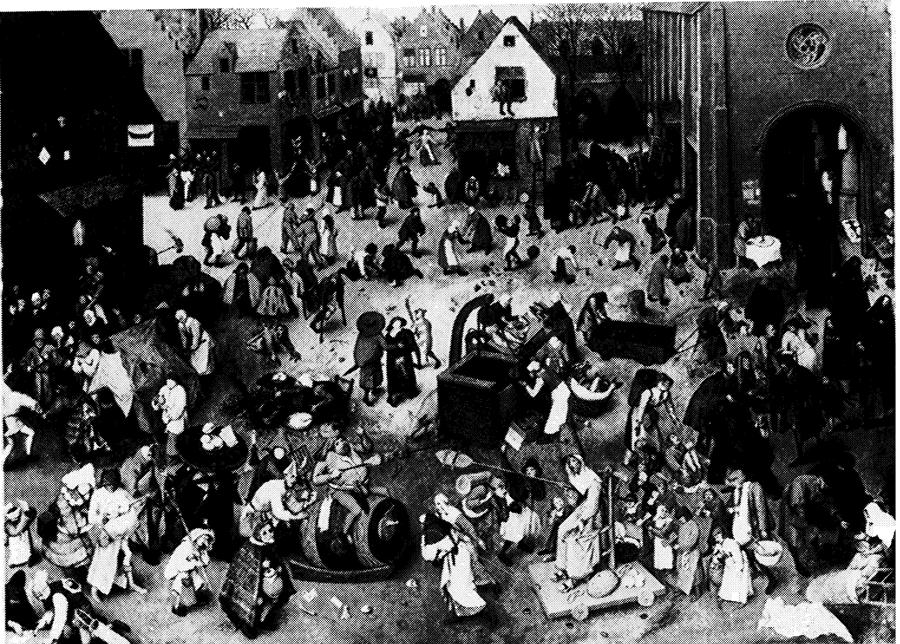
\includegraphics{include/html/images/355_1.png}

PLATE 40. Breughel, Pieter the Elder. \emph{The Battle between Carnival
and Lent}. Courtesy of Kunsthistorisches Museum, Vienna.

\protect\hypertarget{20_ILLUSTRATIONS_FOLLOW_PAGE.xhtmlux5cux23id_36}{}{}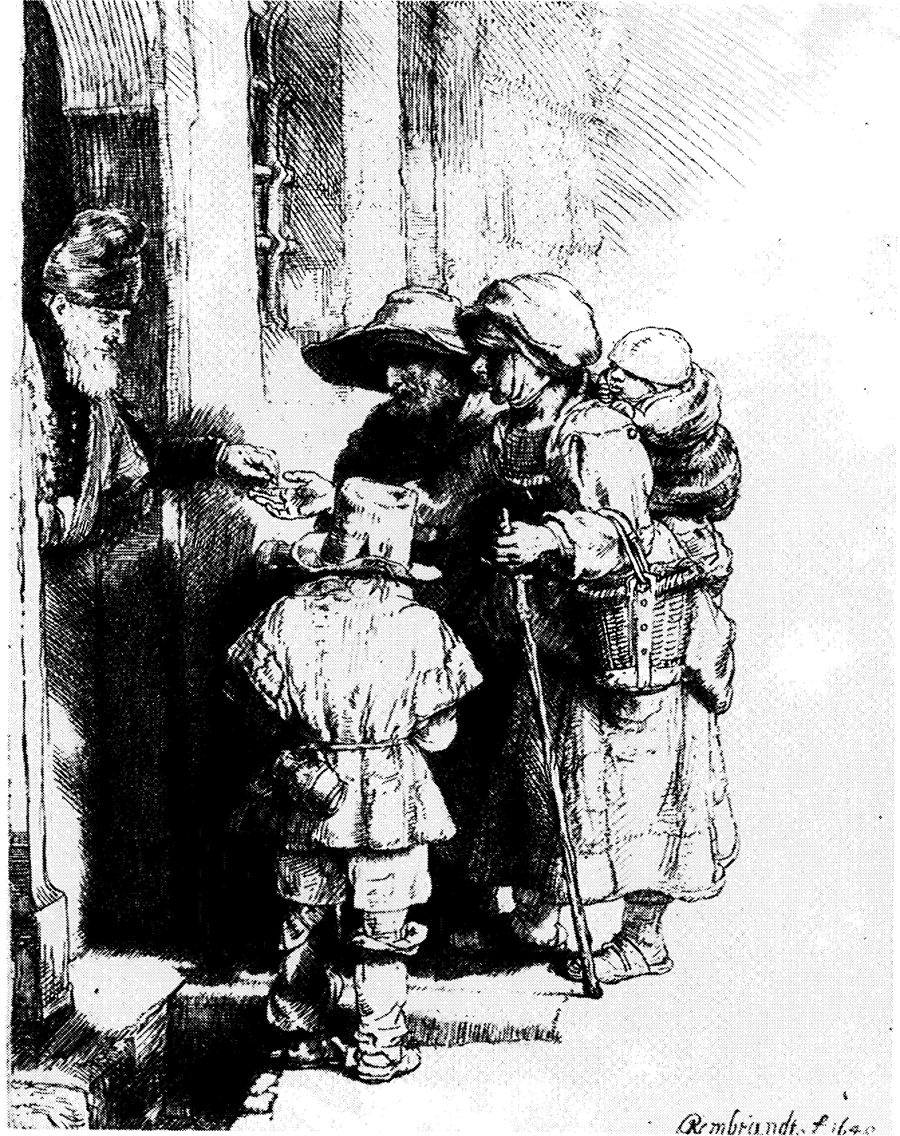
\includegraphics{include/html/images/356_1.png}

PLATE 41. Rembrandt Harmensz van Rijn. \emph{The Beggars}. Courtesy Foto
Marburg/Art Resource, New York.

\protect\hypertarget{20_ILLUSTRATIONS_FOLLOW_PAGE.xhtmlux5cux23id_37}{}{}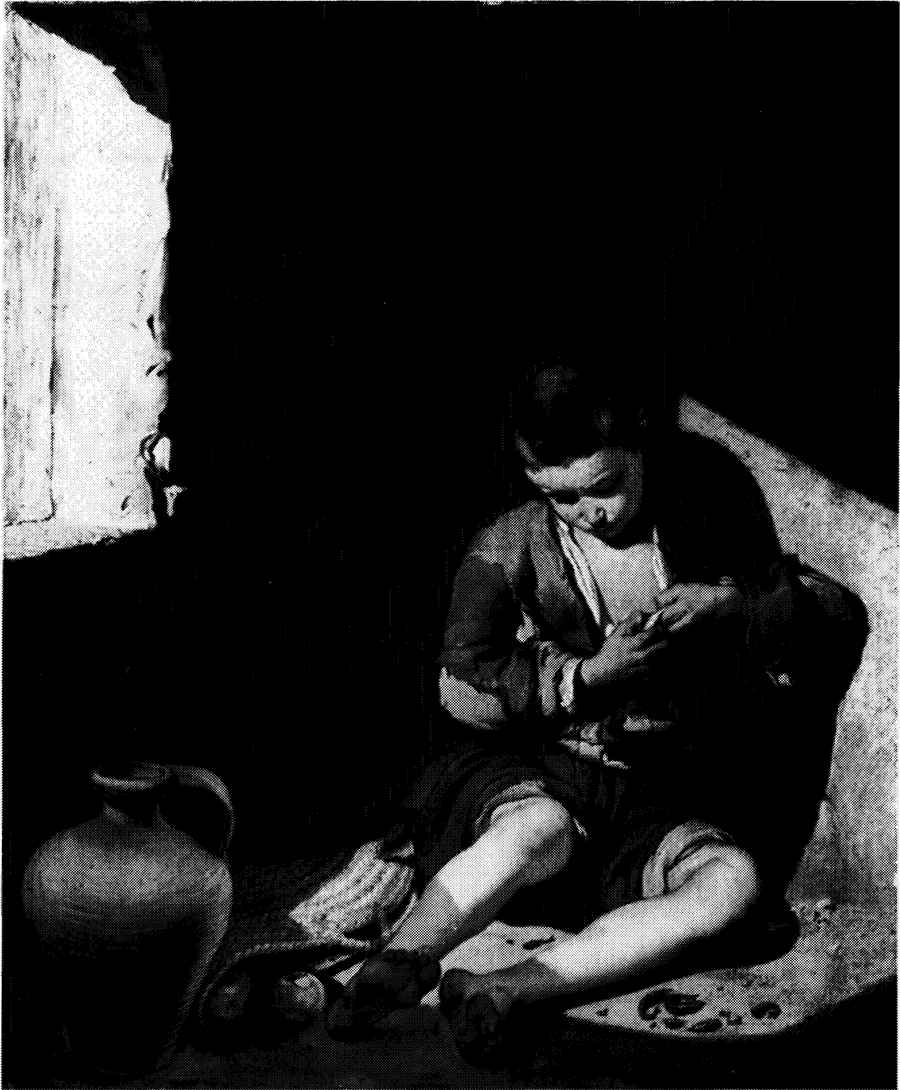
\includegraphics{include/html/images/357_1.png}

PLATE 42. Murillo, Bartolomé. \emph{Beggar Boy}. Louvre, Paris. Cliché
des Musées Nationaux-Paris.

\protect\hypertarget{20_ILLUSTRATIONS_FOLLOW_PAGE.xhtmlux5cux23id_38}{}{}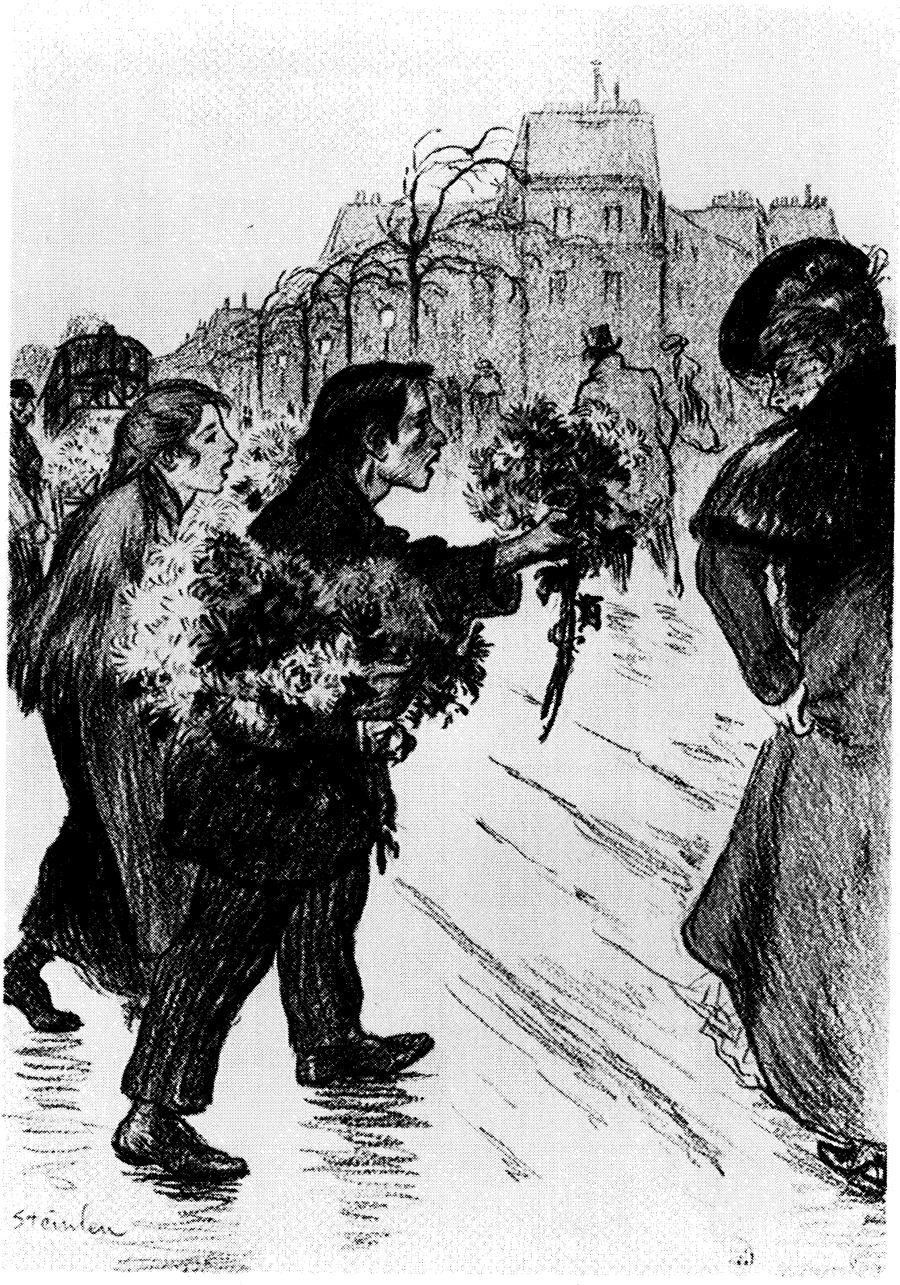
\includegraphics{include/html/images/358_1.png}

PLATE 43. Steinlen, Theophile. \emph{Flower Sellers on the Boulevard}.
Musée de la Ville de Paris, Musée Carnavalet, Paris.

\protect\hypertarget{20_ILLUSTRATIONS_FOLLOW_PAGE.xhtmlux5cux23id_39}{}{}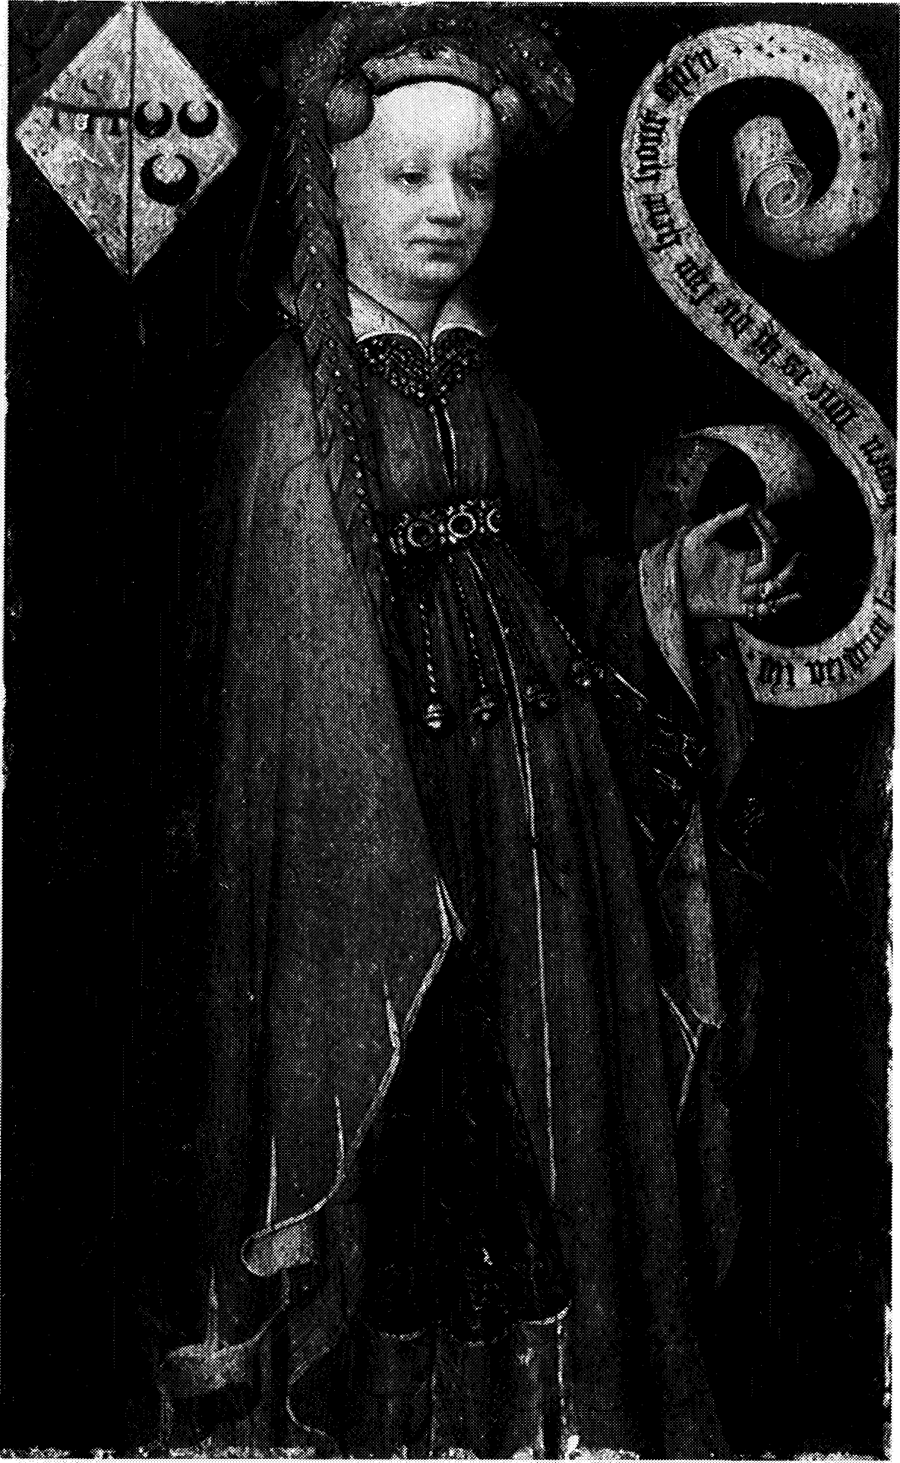
\includegraphics{include/html/images/359_1.png}

PLATE 44. Northern Netherlands School: \emph{Lysbeth van Durenvoode}.
Rijksmuseum, Amsterdam.

\protect\hypertarget{20_ILLUSTRATIONS_FOLLOW_PAGE.xhtmlux5cux23id_40}{}{}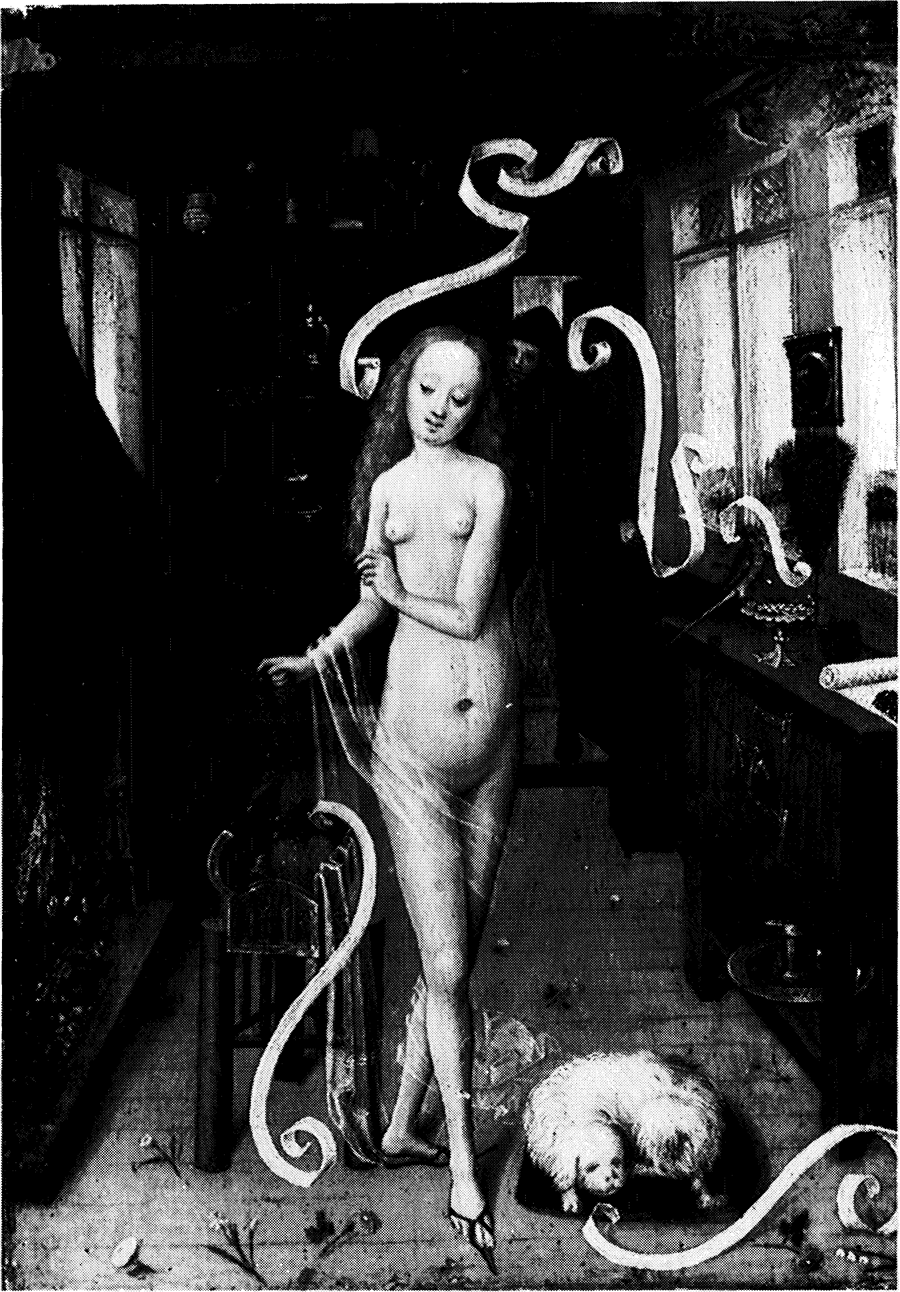
\includegraphics{include/html/images/360_1.png}

PLATE 45. Master of the Bonner Diptych: \emph{Love Magic}. Museum der
Bildenden Künste, Leipzig.

\protect\hypertarget{20_ILLUSTRATIONS_FOLLOW_PAGE.xhtmlux5cux23page_299}{}{}Of
the many works from the hands of the great and not so great artists only
a fraction of a rather special kind have been preserved. These are
primarily tomb monuments, altarpieces, portraits, and miniatures. With
the exception of portraits, only very little survives of secular
painting. Of the ornamental arts and crafts, we have a number of
specific categories: church utensils, clerical vestments, some
furniture. How much would our insight into the character of the art of
the fifteenth century be improved if we could place the bathing scenes
of Jan van Eyck or Rogier van der Weyden or the hunting scenes side by
side with the many pietàs and madonnas. We are hardly able to form any
understanding of the entire field of the applied arts. To do so, we
would have to see the ecclesiastical paraments and the stately robes of
the court, bedecked with precious stones and bells, all together. We
would have to be able to see the splendidly decorated ships of which the
miniatures convey only a highly deficient, mechanical notion. There are
only a few things whose beauty aroused so much enthusiasm in Froissart
as that of
ships.\textsuperscript{\protect\hypertarget{20_ILLUSTRATIONS_FOLLOW_PAGE.xhtmlux5cux23id_453}{\protect\hyperlink{23_NOTES.xhtmlux5cux23page_432}{10}}}
The banners, richly decorated with coats of arms,
\protect\hypertarget{20_ILLUSTRATIONS_FOLLOW_PAGE.xhtmlux5cux23page_300}{}{}fluttering
from the tops of the mast, were sometimes so long that they touched the
water. In the paintings of ships by Peter Breughel these unusually long
and broad streamers can still be seen
(\protect\hyperlink{20_ILLUSTRATIONS_FOLLOW_PAGE.xhtmlux5cux23id_13}{plate
12}). The ship of Philip the Bold, on which Melchior Broederlam worked
in 1387 at Sluis, was covered with blue and gold; large coats of arms
graced the pavilion of the aftercastle. The sails were strewn with
marguerites, the initials of the ducal couple and their slogan, ``Il me
tarde.'' Noblemen vied with one another to see whose ship was most
expensively decorated for the expedition to England. Painters are well
off, says
Froissart,\textsuperscript{\protect\hypertarget{20_ILLUSTRATIONS_FOLLOW_PAGE.xhtmlux5cux23id_451}{\protect\hyperlink{23_NOTES.xhtmlux5cux23id_452}{11}}}
they are able to demand any price, and there are never enough of them.
He claims that many ships had the masts covered with gold leaf. Guy de
la Trémoïlle, in particular, spared no expense: He spent more than two
thousand pounds for gilding. ``L'on ne se povoit de chose adviser pour
luy jolyer, ne deviser, que le seigneur de la Trimouille ne le feist
faire en ses nefs. Et tout ce paioient les povres gens parmy France
.~.~. ``
\protect\hypertarget{20_ILLUSTRATIONS_FOLLOW_PAGE.xhtmlux5cux23id_2661}{\protect\hyperlink{23_NOTES.xhtmlux5cux23id_2662}{*\textsuperscript{4}}}

This taste for splendid extravagance would undoubtedly catch our
attention forcefully if we could see the lost secular decorative arts.
The surviving works of art most decidedly do share that tendency towards
extravagance, but since we value this quality in art least, we pay less
attention to it. We only seek to enjoy the profound beauty of any given
work. Everything that is mere splendor and pomp has lost its attraction
for us. For contemporaries, however, this very pomp and splendor was of
tremendous importance.

French-Burgundian culture of the waning Middle Ages counts among those
cultures in which beauty is replaced by splendor. Late medieval art
reflects the spirit of the late Middle Ages faithfully, a spirit that
had run its course. What we had posited as one of the most important
characteristics of late medieval thought, the depiction of everything
that could be thought down to the smallest detail, the oversaturation of
the mind with an endless system of formal representation, this, too,
constitutes the essence of the art of that time. Art, too, tries to
leave nothing unformed, unpresented, or undecorated. The flamboyant
Gothic is like an endless organ postlude; it breaks down all forms by
this self-analyzing
\protect\hypertarget{20_ILLUSTRATIONS_FOLLOW_PAGE.xhtmlux5cux23page_301}{}{}process;
every detail finds its continuous elaboration, each line its
counterline. It is an unrestrainedly wild overgrowth of the idea by the
form; ornate detail attacks every surface and line. That \emph{horror
vacui}, which may perhaps be identified as a characteristic of end
periods of intellectual development, dominates in this art.

This all means that the boundaries between splendor and beauty become
less distinct. Embellishment and ornamentation no longer serve the
glorification of the naturally beautiful, but rather overgrow and thus
threaten to choke it. The farther the departure from purely pictorial
art, the more unrestrained the wild overgrowth of formal ornamentation
covering content. There is little opportunity for sculpture to engage in
this wild growth of forms as long as it creates freestanding figures:
the statues of the Moses Fountain and the
``plourants''\textsuperscript{\protect\hypertarget{20_ILLUSTRATIONS_FOLLOW_PAGE.xhtmlux5cux23id_449}{\protect\hyperlink{23_NOTES.xhtmlux5cux23id_450}{12}}}
of the tombstones compete, in their strict, simple, naturalness, with
Donatello. But as soon as the task of the art of sculpture is of a
decorative nature or falls into the realm of painting and, bound by the
reduced dimensions of the relief, reproduces entire scenes, sculpture,
too, overindulges in restless, overloaded displays. Those who see the
carvings by Jacques de Baerze at the tabernacle in Dijon next to the
paintings of Broederlam will notice the disharmony between them
(\protect\hyperlink{20_ILLUSTRATIONS_FOLLOW_PAGE.xhtmlux5cux23id_14}{plate
13}). In painting, wherever it is purely representational, simplicity
and quietude dominate; carving, by its very nature decorative, treats
the shaping of figures ornamentally, and one perceives the phenomenon of
forms crowding each other out as something that supplants the quietude
of the painted object. The difference between painting and tapestries is
of the same kind. The art of weaving, even in cases where it assumes a
task of a purely representational nature, by virtue of its set
technique, stands closer to ornamentation and is unable to extricate
itself from the exaggerated need for embellishment. Tapestries are
overcrowded with figures and colors and remain apparently archaic in
form.\textsuperscript{\protect\hypertarget{20_ILLUSTRATIONS_FOLLOW_PAGE.xhtmlux5cux23id_447}{\protect\hyperlink{23_NOTES.xhtmlux5cux23id_448}{13}}}
Departing still further from the pure fine arts, we encounter clothing.
Clothing, too, belongs undeniably to art, but it is part of its very
purpose that allure and ostentation predominate over beauty itself.
Moreover, personal vanity pulls the art of clothing into the sphere of
passion and sensuousness where the qualities that comprise the essence
of high art, balance and harmony, come second.

An extravagance like that found in the style of dress between 1350 and
1480 has not been experienced in later ages, at least not
\protect\hypertarget{20_ILLUSTRATIONS_FOLLOW_PAGE.xhtmlux5cux23page_302}{}{}in
such a general and sustained way. Certainly there have been extravagant
fashions in later times, such as the dress of the mercenaries around
1520 and aristocratic French costume in 1660, but the unrestrained
exaggeration and overprofusion so characteristic of French-Burgundian
dress for a century has no parallel. In their dress we are privileged to
observe what the sense of beauty of that age, left to its own
undisturbed impulses, would accomplish. A court costume is overburdened
with hundreds of precious stones and all its proportions are exaggerated
to a ridiculous degree; the headdress of women assumes the sugarloaf
form of the hennin; natural hair is hidden or removed at the temples and
from the area of the forehead at the hairline, so that the curiously
vaulted foreheads that were considered beautiful were prominently
displayed. The décolletage began abruptly. Male garments, however,
displayed still more numerous extravagances; most striking of all, the
elongated toes of the shoes, the \emph{poulaines}, which the knights at
Nicopolis\textsuperscript{\protect\hypertarget{20_ILLUSTRATIONS_FOLLOW_PAGE.xhtmlux5cux23id_445}{\protect\hyperlink{23_NOTES.xhtmlux5cux23id_446}{14}}}
had to cut off in order to be able to flee, the narrow waists, the
balloon-like puffed-up sleeves that rose at the shoulders, the
houpelandes dangling to the feet, and the short jackets that barely
covered the hips, the tall caps or hats narrowing at the tips or shaped
like a cylinder, the bonnets wondrously draped around the head
reminiscent of a cock's comb or a flickering flame. The more festive the
more extravagant, since all this beauty was equated with splendor,
stateliness,
\emph{estat}.\textsuperscript{\protect\hypertarget{20_ILLUSTRATIONS_FOLLOW_PAGE.xhtmlux5cux23id_443}{\protect\hyperlink{23_NOTES.xhtmlux5cux23id_444}{15}}}
The mourning dress that Philip the Good wears after the murder of his
father while receiving the King of England is so long that it trails
from the tall horse he is riding all the way to the
ground.\textsuperscript{\protect\hypertarget{20_ILLUSTRATIONS_FOLLOW_PAGE.xhtmlux5cux23id_441}{\protect\hyperlink{23_NOTES.xhtmlux5cux23id_442}{16}}}

All this wasteful splendor reaches its climax in the festivities of the
court. Everyone remembers the descriptions of the Burgundian court
festivities, such as the banquet at Lille in 1454, where the guests took
their vows to participate in the crusade against the Turks while the
pheasants were being served, or the wedding feast of Charles the Bold
and Margaret of York at Bruges in
1468.\textsuperscript{\protect\hypertarget{20_ILLUSTRATIONS_FOLLOW_PAGE.xhtmlux5cux23id_439}{\protect\hyperlink{23_NOTES.xhtmlux5cux23id_440}{17}}}
We cannot imagine a greater distance than that which exists between the
consecrated atmosphere of the Ghent and Louvain altars and these
expressions of barbaric princely ostentation. The descriptions of all
those \emph{estremets} with pastry from within which musicians
performed, the overly ornate ships and castles, the monkeys, whales,
giants, and dwarfs, and all the worn allegory belonging to them force us
to see them as unusually insipid performances.

\protect\hypertarget{20_ILLUSTRATIONS_FOLLOW_PAGE.xhtmlux5cux23page_303}{}{}However,
isn't the distance we perceive between the two extremes of church art
and the art of the court festivities easily exaggerated in more than one
respect? First of all, we have to be clear about the function that the
festivity served in society. It still had the purpose that it had among
primitive peoples; that is, to be the sovereign expression of the
culture, to be the form in which the highest joy of life was expressed
by the community, and to express the sense of that community. During
times of great social renewal, such as at the time of the French
Revolution, festivities sometimes regain that important social and
aesthetic function.

Modern man is in a position to seek individually the confirmation of his
view of life and the purest enjoyment of his \emph{joie de vivre} during
any moment of leisure in self-chosen relaxations. But an age in which
the spiritual luxuries are still poorly distributed and less accessible
requires for the purpose of renewal a communal act: the festival. The
greater the contrast with the misery of daily life, the more
indispensable the festival and the stronger the means required to bestow
splendor on life by virtue of the ecstasy of beauty and enjoyment that
lights up the darkness of reality. The fifteenth century was an age of
great emotional depression and thorough pessimism. We have already
mentioned earlier the permanent pressure from injustice and violence,
hell and damnation, pestilence, fire and hunger, Satan and the witches,
under which the century lived. Mankind in its wretchedness needed more
than the daily repeated promise of heavenly bliss and God's watchful
care and benevolence: from time to time a glorious, solemn, and communal
affirmation of the beauty of life was required. The enjoyment of life in
its primary forms---play, love, drink, dance, and song---does not
suffice. Life has to be ennobled through beauty, to be stylized in a
social expression of the joy of life. For the individual, relief through
the reading of books, listening to music, seeing art, or enjoying nature
was still out of reach; books were too expensive, nature too dangerous,
and art was no more than a small part of the festival.

The folk festival had only song and dance for its original sources of
beauty. For the beauty of color and form folk festivals based themselves
on church festivals, which had both in abundance, and usually took place
immediately after a church festival. The separation of the urban
festival from the church form, and its establishment of a decor of its
own, took place throughout the entire
fif\protect\hypertarget{20_ILLUSTRATIONS_FOLLOW_PAGE.xhtmlux5cux23page_304}{}{}teenth
century through the labor of the rhetoricians. Prior to this time, the
princely courts had been in a position both to arrange a purely secular
festival with an attendant display of art and to bestow on the festival
a splendor of its own. But display and splendor are not sufficient for
festivals; nothing is as indispensable for them as style.

The church festival possessed style because of its liturgy. In a
beautiful communal social gesture the church festivals always managed to
give moving expression to a lofty idea. The sacred dignity and noble
stateliness of the ceremonies were not destroyed even by the most
extreme overgrowth of festive details, which bordered on the burlesque.
But from where were court festivals to obtain style? On which conception
was it to be based?---The answer could be none other than the chivalric
ideal, because the entire life of the court was based on it. Was the
chivalric ideal tied to a style, to a liturgy, so to speak? Indeed;
everything related to the act of bestowing knighthood, the rules of
orders, tournaments, \emph{préséance, hommage}, and service, the entire
game of the kings at arms, heralds, coats of arms, constituted the
style. To the degree the court festival was based on those elements, it
most decidedly possessed in the eyes of contemporaries a greatly
elevated style. Strong sensitivity to the stylish festive air of the
ceremonial procedure frequently comes naturally to modern man,
independent of all the awe with which all matters aristocratic or
monarchic are seen. How much more so it must have been for those who
were still captivated by the delusion of that chivalric ideal whenever
they encountered the pompous display of costumes with their long trains
and glittering colors!

But court festivals aspired to more. They wanted to present the dream of
the heroic life in its extreme form. This is where the style failed. The
entire apparatus of knightly fancy and splendor was no longer filled
with real life. Everything had become much too literary, a sickly
renaissance, an empty convention. The inner decay of the form of life
remained hidden under the overload of glamour and etiquette. The
chivalric idea of the fifteenth century revels in a romanticism that is
hollow and worn throughout. And that was the source from which the court
festival was supposed to derive the inspiration for its performances and
presentations. How could it create a style from such a styleless,
undisciplined, and stale literature as that of chivalric romanticism in
its decay?

\protect\hypertarget{20_ILLUSTRATIONS_FOLLOW_PAGE.xhtmlux5cux23page_305}{}{}The
aesthetic value of the \emph{entremets} should be seen in this light:
They were applied literature. Actually, this was the only way this
literature could be made bearable, since in the \emph{entremets} the
fleeting, superficial shapes of all the colorful literary dream figures
had to make room for the necessity of the material representation.

The heavy barbarian seriousness evident in all this fits well into the
Burgundian court, which seemed to have lost the lighter and more
harmonious French spirit through its contact with the North. All the
tremendous display is taken solemnly and seriously. The great festivity
of the duke at Lille was both the end and the climax of a number of
banquets given by the court nobility in competition with each other. All
this had started quite simply and with little expense; the number of
guests and the luxury of the menus and \emph{entremets} were gradually
increased. By being offered a wreath by his host, a guest was designated
to take his turn as successor; in this manner the knights were followed
by the great lords and the great lords by the princes, all this with
steadily increasing expense and stateliness, until it was finally the
turn of the duke himself. But Philip intended to hold more than a
splendid feast; he intended to collect vows for the crusade against the
Turks for the reconquest of Constantinople, which had fallen a year
earlier. This was the officially proclaimed goal of the duke's life. To
prepare for the feast, he appointed a commission with the knight of the
Fleece, Jean de Lannoy, as its leader. Olivier de la Marche, too, was a
member. Whenever he comes to this issue in his memoirs he becomes very
solemn: ``Pour ce que grandes et honnorables oeuvres désirent loingtaine
renomée et perpétuelle
mémoire.''\protect\hypertarget{20_ILLUSTRATIONS_FOLLOW_PAGE.xhtmlux5cux23id_2663}{\protect\hyperlink{23_NOTES.xhtmlux5cux23id_2664}{*\textsuperscript{5}}}
These are the words with which he begins to reminisce about those great
events.\textsuperscript{\protect\hypertarget{20_ILLUSTRATIONS_FOLLOW_PAGE.xhtmlux5cux23id_437}{\protect\hyperlink{23_NOTES.xhtmlux5cux23id_438}{18}}}
The first councillors, who were closest to the duke, regularly attended
the deliberations: even Chancellor Rolin and Antoine de Croy, the First
Chamberlain, were consulted before agreement was reached where ``les
cérémonies et les mistères'' should be held.

All these beautiful events have been described so often that there is no
need to do so here. Some had even crossed the channel to witness the
spectacle. Joining the guests were innumerable noble onlookers, the
majority of whom were masked. First the guests took a stroll to admire
the splendid stationary displays; then came
\protect\hypertarget{20_ILLUSTRATIONS_FOLLOW_PAGE.xhtmlux5cux23page_306}{}{}the
performances with living persons and \emph{tableaux vivants}. Olivier
himself played the leading role of Sainte Eglise when she entered during
the most important scene inside a tower placed on the back of an
elephant led by a giant Turk. The tables were given the most marvelous
decorations: a manned
carrack\textsuperscript{\protect\hypertarget{20_ILLUSTRATIONS_FOLLOW_PAGE.xhtmlux5cux23id_435}{\protect\hyperlink{23_NOTES.xhtmlux5cux23id_436}{19}}}
with full sails, a meadow with trees, a spring, rocks, and a picture of
St. Andreas, Lusignan Castle with the fairy Melusine, a windmill and a
bird-shooting scene, a forest with moving wild animals, and, finally,
the church with an organ and singers that, alternating with the
twenty-eight-man orchestra that was sitting in a pie, offered musical
performances.

What matters here is the degree of taste or tastelessness that is found
in all this. The subject matter itself is nothing but a loose mixture of
mythological, allegorical, and moralizing images, but what about the
execution? There is no doubt that the effect was largely sought through
extravagance. The Tower of Gorkum that served as ostentatious table
decoration during a 1468 wedding celebration was forty-six feet
tall.\textsuperscript{\protect\hypertarget{20_ILLUSTRATIONS_FOLLOW_PAGE.xhtmlux5cux23id_433}{\protect\hyperlink{23_NOTES.xhtmlux5cux23id_434}{20}}}
La Marche reports about a whale fashioned for the same occasion: ``Et
certes ce fut un moult bel entremectz, car il y avoit dedans plus de
quarante
personnes.''\textsuperscript{\protect\hypertarget{20_ILLUSTRATIONS_FOLLOW_PAGE.xhtmlux5cux23id_431}{\protect\hyperlink{23_NOTES.xhtmlux5cux23id_432}{21}}}\protect\hypertarget{20_ILLUSTRATIONS_FOLLOW_PAGE.xhtmlux5cux23id_2665}{\protect\hyperlink{23_NOTES.xhtmlux5cux23id_2666}{*\textsuperscript{6}}}
As to the miracles of mechanical gadgetry, such as the living birds that
fly out of the mouth of the dragon with whom Hercules does battle and
other such astonishing contraptions, it is difficult to associate them
with any notion of art. The comic element is only poorly represented in
them. From inside the Gorkum tower, wild boars play trumpets, goats
perform a motet, wolves play the flute, four large asses perform as
singers---and do so before Charles the Bold, who was a connoisseur of
music of some stature.

I do not wish to cast doubt that, in spite of everything, there were
found among all the displays of the festival, particularly among the
sculptural pieces, a good many genuine works of art alongside the
predominantly silly ostentation. We should remember that the people who
delighted in this gargantuan splendor and wasted serious thought on it
were the same people who commissioned the works of Jan van Eyck and
Rogier van der Weyden. The duke himself was their patron, as was Rolin,
the donor of the altars of Beaune
(\protect\hyperlink{20_ILLUSTRATIONS_FOLLOW_PAGE.xhtmlux5cux23id_2298}{plate
14}) and Autun
(\protect\hyperlink{20_ILLUSTRATIONS_FOLLOW_PAGE.xhtmlux5cux23id_15}{plates
15},
\protect\hyperlink{20_ILLUSTRATIONS_FOLLOW_PAGE.xhtmlux5cux23id_16}{16}),
and Jean
\protect\hypertarget{20_ILLUSTRATIONS_FOLLOW_PAGE.xhtmlux5cux23page_307}{}{}Chevrot,
who was the patron of Rogier's \emph{Seven Sacraments}
(\protect\hyperlink{20_ILLUSTRATIONS_FOLLOW_PAGE.xhtmlux5cux23id_17}{plate
17}), and many others, such as Lannoy. It is even more significant that
the creators of these and similar ostentations were these very same
painters. Though it happens that we have no definite information about
Jan van Eyck or Rogier, we do know it to be a fact that others, Colard
Marmion, Simon Marmion, and Jacques Daret, for example, often had a hand
in such festivals. For the festival in 1468, the date of which was
unexpectedly moved up, the entire guild of painters was mobilized to
assure completion; in great haste journeymen from Ghent, Brussels,
Louvain, Thirlemont, Bergen, Quesnoy, Valenciennes, Douai, Cambrai,
Arras, Lille, Ypres, Courtray, and Oudenarde were dispatched to
Bruges.\textsuperscript{\protect\hypertarget{20_ILLUSTRATIONS_FOLLOW_PAGE.xhtmlux5cux23id_429}{\protect\hyperlink{23_NOTES.xhtmlux5cux23id_430}{22}}}
What was produced by their hands cannot have been completely ugly. One
would readily exchange many a mediocre altarpiece for the thirty fully
equipped ships, complete with the coats of arms of the ducal lords, of
the banquet of 1468, the sixty women in different regional
costumes\textsuperscript{\protect\hypertarget{20_ILLUSTRATIONS_FOLLOW_PAGE.xhtmlux5cux23id_427}{\protect\hyperlink{23_NOTES.xhtmlux5cux23id_428}{23}}}
holding fruit baskets and bird cages, and the windmills and bird
catchers.

Even at the risk of sacrilege, it is tempting to go one step further and
assert that on occasion we have to keep in mind this lost art of table
decoration, now completely vanished, in order to better understand Claus
Sluter\textsuperscript{\protect\hypertarget{20_ILLUSTRATIONS_FOLLOW_PAGE.xhtmlux5cux23id_425}{\protect\hyperlink{23_NOTES.xhtmlux5cux23id_426}{24}}}
and others like him.

Among the other arts, that of funeral sculpture served a clearly
practical function. The task facing the sculptors charged with creating
the tomb monuments for the Burgundian dukes was not one of imaginative
beauty, but was rather concerned with glorifying princely grandeur.
Their task was much more strictly limited and more precisely prescribed
than that of the painters, who in commissioned works were allowed to
give much freer reign to their creative urges and who could paint
whatever they wanted when not working on a commission. The sculptor of
that age probably did little work outside of his commissions and the
motifs of his work were limited in number and tied to a strong
tradition. Sculptors were then much more tightly dependent on the dukes
than the painters. The two great Dutch artists who were enticed out of
their country by the magnet of French artistic life were totally
monopolized by the duke of Burgundy. Sluter lived in a house in Dijon
assigned and furnished for him by the
duke.\textsuperscript{\protect\hypertarget{20_ILLUSTRATIONS_FOLLOW_PAGE.xhtmlux5cux23id_423}{\protect\hyperlink{23_NOTES.xhtmlux5cux23id_424}{25}}}
He lived there like a great lord, but at the same time like an employee
of the court. The court rank ``varlet de chambre de monsegneur le
duc\protect\hypertarget{20_ILLUSTRATIONS_FOLLOW_PAGE.xhtmlux5cux23page_308}{}{}de
Bourgogne,''\protect\hypertarget{20_ILLUSTRATIONS_FOLLOW_PAGE.xhtmlux5cux23id_2667}{\protect\hyperlink{23_NOTES.xhtmlux5cux23id_2668}{*\textsuperscript{7}}}
which Sluter shared with his cousin Claes van de Werve and Jan van Eyck,
had an authoritative meaning for the sculptors. Claes van de Werve, who
continued Sluter's work, became one of the tragic victims of art in the
service of the court: kept in Dijon year in and out in order to complete
the tomb monument of John the Fearless
(\protect\hyperlink{20_ILLUSTRATIONS_FOLLOW_PAGE.xhtmlux5cux23id_18}{plate
18}), a task for which there were never funds available, his splendidly
promising career wasted away in futile waiting and he died having never
been able to finish his task.

This relationship of servitude, however, runs contrary to the fact that
it is in the nature of the art of sculpture always to approach a certain
peak of simplicity and freedom, primarily because of the limited nature
of its means, its material, and its subject matter. We call this peak of
simplicity and freedom classicism. It is reached as soon as one of the
great masters, even be it only one, regardless of time and place, guides
the chisel. No matter what the task the age intends to force upon the
art of sculpture, the human figure and its clothing allow for only a few
variations in their depiction in wood and stone. The differences between
the Roman portrait sculpture of the Imperial period, Goujon and Colombe
in the sixteenth century, and Houdon and Pajou in the eighteenth are
much smaller than in any other field of art.

The art of Sluter, and those like him, shares in the eternal nature of
the art of sculpture. And yet .~.~. we don't perceive Sluter's works as
they really were and were intended to be. As soon as one visualizes the
Moses Fountain, just in the manner it delighted its contemporaries at
the time when the papal legate (1418) granted absolution to anyone who
visited it with pious intentions---one realizes why we dared to mention
Sluter's art and that of the \emph{entre-mets} in one breath.

The Moses Fountain is known only as a fragment
(\protect\hyperlink{20_ILLUSTRATIONS_FOLLOW_PAGE.xhtmlux5cux23id_19}{plate
20}). The first duke of Burgundy wished to see the fountain, surmounted
by an image of the Mount of Calvary, put into the yard of the
Carthusians in his beloved Champmol. The main part of the work is
comprised of the figure of the crucified Christ with Mary, John, and the
Magdalen placed at the foot of the cross. The work had already vanished,
for the most part, prior to the Revolution, which so irretrievably
disfigured the Champmol. Below the central part,
\protect\hypertarget{20_ILLUSTRATIONS_FOLLOW_PAGE.xhtmlux5cux23page_309}{}{}and
surrounding the base that is held up around the edge by angels, stand
the six figures from the Old Testament who prophesied the death of the
Messiah: Moses, David, Isaiah, Jeremiah, Daniel, and Zachariah, each
with an attached banderole on which the prophetic texts can be read. The
entire depiction has to the highest degree the character of a
performance. This is not so much because of the fact that the
\emph{tableaux vivants} or ``personnages,'' which during processions and
banquets usually had figures with such banderoles attached to them, or
that the Messiah prophecies from the Old Testament were the most
important subjects of such representations, as because of the fact that
this depiction has an unusually strong verbal effect about it. The words
of the inscriptions have an emphasized place of importance. We only
reach a full understanding of the work if we completely absorb the
sacred import of those
texts.\textsuperscript{\protect\hypertarget{20_ILLUSTRATIONS_FOLLOW_PAGE.xhtmlux5cux23id_421}{\protect\hyperlink{23_NOTES.xhtmlux5cux23id_422}{26}}}
``Immolabit enum universa multitudo filiorum Israel ad vesperam,'' reads
Moses's dictum. ``Foderunt manus meas et pedes meos, dinumeraverunt
omnia ossa mea,'' is the citation from the Psalms of David. ``Sicut ovis
ad occisionem ducetur et quasi agnus coram tondente se obmutescet et non
aperiet os suum,'' from Isaiah. ``O vos omnes qui transitis per viam,
attendite et videte si est dolor sicut dolor meus,'' Jeremiah. ``Post
hebdomades sexaginta duas occidetur Christus,'' Daniel. ``Appenderunt
mercedem meam triginta argenteos,'' Zachariah. So reads the lament,
rising in six voices around the base of the cross. This is the essential
feature of the work. And the connection between the figures and the text
is stressed with such emphasis, there is something so compelling in the
gesture of one figure and the face of another, that the entire group is
almost in danger of losing the ataraxia that is the privilege of all
great sculpture. The viewer is addressed almost too directly. Sluter
knew, as few artists have, how to express the sanctity of his subject
matter. But, from the point of view of pure art, this weight of sanctity
constitutes something overdone. Compared with Michelangelo's tomb
figures, Sluter's prophets are too expressive, too personal. We would
perhaps consider this criticism to be doubly meritorious if more than
only the head and torso of the main figure of Christ in his rigid
majesty had been preserved. All we can see is how the angels, those
wondrously poetic angels who in their naive grace are so infinitely more
angelic than the angels of Van Eyck, direct the devotion of the prophets
to the scene above them.

The strongly representative character of the Calvary of
Champ\protect\hypertarget{20_ILLUSTRATIONS_FOLLOW_PAGE.xhtmlux5cux23page_310}{}{}mol
is based, however, on something other than its purely sculptural
qualities; that is, on the splendor in which the entire work was cast.
It should be imagined as if it were painted in polychrome by Jean
Maelweel and gilded by Hermann of
Cologne.\textsuperscript{\protect\hypertarget{20_ILLUSTRATIONS_FOLLOW_PAGE.xhtmlux5cux23id_419}{\protect\hyperlink{23_NOTES.xhtmlux5cux23id_420}{27}}}
Not a single colorful or dramatic effect had been left out. The prophets
in their golden coats were standing on green pedestals; Moses and
Zachariah in red robes, their coats lined in blue; David entirely in
blue with golden stars; Jeremiah in dark blue; Jessiah, the saddest of
them all, in brocade. Golden suns and initials filled the empty areas.
Add to all this the coats of arms! The proud coats of arms of the ducal
region gleamed not only on the shaft of the base below the prophets, but
even on the crosspiece of the great, entirely gilded cross---on its
extensions shaped like capitals had been placed the coats of arms of
Burgundy and Flanders! This, perhaps more than the gilded copper pair of
glasses, supplied by Hannequin de Hacht for the nose of Jeremiah,
testifies to the spirit that gave rise to this grand ducal work of art.

The dependence of this work on its princely sponsors contributes to a
somewhat tragic and elevated element because of the greatness by means
of which the artist manages to evade the restrictions of his commission.
The representation of the ``Plourants'' around the sarcophagus had
become obligatory in Burgundian funeral art long
ago.\textsuperscript{\protect\hypertarget{20_ILLUSTRATIONS_FOLLOW_PAGE.xhtmlux5cux23id_417}{\protect\hyperlink{23_NOTES.xhtmlux5cux23id_418}{28}}}
Its aim was not a creative expression of pain in all its depths, but
rather only a very realistic depiction of a part of the actual
procession that had accompanied the body to the grave and with all the
dignitaries readily recognizable. How skillfully Sluter and his
assistants managed to turn this motif into a profound and dignified
depiction of grief, into a funeral march in stone!

But this may perhaps be overstating the assumption of disharmony between
sponsor and artist. It is not entirely certain that it was not Sluter
himself who found the pair of glasses on Jeremiah to be a great idea.
Taste and tastelessness were, so to speak, not separated in the minds of
that age; the genuine appreciation of art and the infatuation with pomp
and curiosities had not yet parted company. The naive imagination was
still able to enjoy without embarrassment that which was bizarre as if
it were beautiful. A collection such as that in the Green Vault in
Dresden displays the separated \emph{caput mortuum} that had once been a
whole with the princely art collections. In Hesdin Castle, which was
both a treasure house of art and a pleasure garden filled with those
mechanical
\protect\hypertarget{20_ILLUSTRATIONS_FOLLOW_PAGE.xhtmlux5cux23page_311}{}{}amusements,
\emph{engins d'esbatement}, Caxton came across a room decorated with
paintings depicting the story of Jason, the hero of the Golden Fleece.
For the sake of greater effect, lightning, thunder, snow, and rain
making implements were attached in imitation of Medea's magic
tricks.\textsuperscript{\protect\hypertarget{20_ILLUSTRATIONS_FOLLOW_PAGE.xhtmlux5cux23id_415}{\protect\hyperlink{23_NOTES.xhtmlux5cux23id_416}{29}}}

Imagination was also freely indulged in creating the performances, the
\emph{personnages}, which were placed on street corners during princely
entry processions. During the 1389 entry into Paris of Isabella of
Bavaria as wife of Charles VI, a white stag with gilded antlers and a
crown around its
neck\textsuperscript{\protect\hypertarget{20_ILLUSTRATIONS_FOLLOW_PAGE.xhtmlux5cux23id_413}{\protect\hyperlink{23_NOTES.xhtmlux5cux23id_414}{30}}}
was placed among the holy scenes. The stag rested on a \emph{lit de
justice} and moved his eyes, antlers, feet, and, to conclude, raised a
sword. During the same procession an angel ``par engins bien
faits''\protect\hypertarget{20_ILLUSTRATIONS_FOLLOW_PAGE.xhtmlux5cux23id_2669}{\protect\hyperlink{23_NOTES.xhtmlux5cux23id_2670}{*\textsuperscript{8}}}
descended from the tower of Notre Dame, entered through a gap in the
blue taffeta canopy covering the entire bridge just at the moment the
queen passed by, placed a crown on her head and disappeared in the same
way it had arrived ``comme s'il s'en fust retourné de soy mesmes au
ciel.''\textsuperscript{\protect\hypertarget{20_ILLUSTRATIONS_FOLLOW_PAGE.xhtmlux5cux23id_411}{\protect\hyperlink{23_NOTES.xhtmlux5cux23id_412}{31}}}\protect\hypertarget{20_ILLUSTRATIONS_FOLLOW_PAGE.xhtmlux5cux23id_2671}{\protect\hyperlink{23_NOTES.xhtmlux5cux23id_2672}{†\textsuperscript{9}}}
Philip the Good is presented with a similarly descending
maiden\textsuperscript{\protect\hypertarget{20_ILLUSTRATIONS_FOLLOW_PAGE.xhtmlux5cux23id_409}{\protect\hyperlink{23_NOTES.xhtmlux5cux23id_410}{32}}}
during an entry into Ghent, as is Charles VII in Reims in
1484.\textsuperscript{\protect\hypertarget{20_ILLUSTRATIONS_FOLLOW_PAGE.xhtmlux5cux23id_407}{\protect\hyperlink{23_NOTES.xhtmlux5cux23id_408}{33}}}
We are hard put to imagine anything more silly than a so-called
pantomime horse moved by a man inside, but during the fifteenth century
this was apparently not the case. In any event, Le Fèvre de Saint Remy
reports, without a trace of ridicule, about a performance by four
trumpeters and twelve noblemen ``sur chevaulx de artifice,'' ``saillans
et poursaillians tellement que belle chose estoit à
veoir.''\textsuperscript{\protect\hypertarget{20_ILLUSTRATIONS_FOLLOW_PAGE.xhtmlux5cux23id_405}{\protect\hyperlink{23_NOTES.xhtmlux5cux23id_406}{34}}}\protect\hypertarget{20_ILLUSTRATIONS_FOLLOW_PAGE.xhtmlux5cux23id_2673}{\protect\hyperlink{23_NOTES.xhtmlux5cux23id_2674}{‡\textsuperscript{10}}}

The separation of all that bizarre decoration, which has vanished
without a trace, from the individual works of art that have been
preserved, a separation that our appreciation of art demands and that
has been aided by the all destroying passage of time, hardly existed for
contemporaries. The artistic life of the Burgundian age was still
entirely determined by the forms of social life. Art served. It had
primarily a social function; this was primarily to display splendor and
to emphasize the importance of the individual, not the artist but rather
the donor. This is not contradicted by the fact
\protect\hypertarget{20_ILLUSTRATIONS_FOLLOW_PAGE.xhtmlux5cux23page_312}{}{}that
in church art, pompous splendor serves to direct pious thoughts upward
and that the donor, out of a pious impulse, puts his own figure in the
foreground. On the other hand, the art of secular painting is not always
as luxuriant and arrogant as would be suitable for bloated courtly life.
Too much is missing of the entire environment in which art existed for a
clear understanding of the manner in which art and life touched and
dissolved in each other. Moreover, our knowledge of this art itself is
much too fragmentary for that purpose. It is not court and church alone
that comprise the life of that age.

This is the reason for the special importance of the few works of art in
which something of the life outside those two spheres finds its
expression. One of these works radiates in its own peerless delight: the
portrait of the Arnolfini \emph{Marriage}
(\protect\hyperlink{20_ILLUSTRATIONS_FOLLOW_PAGE.xhtmlux5cux23id_20}{plate
21}). It represents the art of the fifteenth century in its purest form
and allows us to come closest to the enigmatic personality of the
painter Jan van Eyck. Painting the portrait did not require that he
reproduce the splendid majesty of God nor sense the haughtiness of the
nobleman: he painted his friends on the occasion of their wedding. Was
the subject of the painting really Jean Arnoulphin, as he was called in
Flanders, the merchant from Lucca? This face, which Jan van Eyck painted
twice,\textsuperscript{\protect\hypertarget{20_ILLUSTRATIONS_FOLLOW_PAGE.xhtmlux5cux23id_403}{\protect\hyperlink{23_NOTES.xhtmlux5cux23id_404}{35}}}
is not at all Italian. But the title of the painting as \emph{Hernoul le
fin avec sa femme dedens une chambre}, in the
1516\textsuperscript{\protect\hypertarget{20_ILLUSTRATIONS_FOLLOW_PAGE.xhtmlux5cux23id_401}{\protect\hyperlink{23_NOTES.xhtmlux5cux23id_402}{36}}}
inventory of paintings belonging to Margaret of Austria, provides strong
support for the assumption that he is Arnolfini. In that case, the
painting should not actually be called a ``bourgeois portrait,'' since
Arnolfini was a highly placed individual who repeatedly served as
adviser to the ducal government in important matters. Be that as it may,
the man depicted here was a friend of Jan van Eyck. This is shown by the
delicately phrased inscription above the mirror with which the painter
has signed his work: ``Johannes de Eyck fuit his, 1434.'' Jan van Eyck
was here. Just a short time ago. The deep silence of the chamber still
reverberates with the sound of his voice. The intimate tenderness and
the calm peace, which we are to meet again only in Rembrandt, are
encased in this work as if it were, so to speak, Jan's own heart. All of
a sudden, that evening during the Middle Ages is brought back to us, an
evening we know of, but so often seek in vain in literature, in history,
and in the life of faith of that age: the happy, noble, pure,
\protect\hypertarget{20_ILLUSTRATIONS_FOLLOW_PAGE.xhtmlux5cux23page_313}{}{}and
simple medieval age of folk song and church music. How far they are,
that loud laughter and unrestrained passion!

At this moment perhaps we can see in our imagination Jan van Eyck, who
stood outside the tension-filled, vibrant life of his time, a simple
man, a dreamer who went through life with his head bowed, looking inside
himself. Caution!---or this will turn out like an art-historical novel
about how the duke's ``varlet de chambre'' served his high lord
reluctantly, how his companions, full of pain, had to deny their high
art so that they could join the work of staging courtly festivities and
equipping fleets!

There is nothing in our possession that could justify any such notion.
The art of the Van Eycks', which we so admire, stood right in the middle
of the courtly life that is so repugnant to us. The little we know of
the life of those painters makes them appear to be men of the great
world. The duke of Berry is on the best of terms with his painters.
Froissart met him in intimate conversation with André Beauneveu in his
marvelous castle at Mehun sur
Yevre.\textsuperscript{\protect\hypertarget{20_ILLUSTRATIONS_FOLLOW_PAGE.xhtmlux5cux23id_399}{\protect\hyperlink{23_NOTES.xhtmlux5cux23id_400}{37}}}
The three brothers from Limburg, the great illustrators, delight the
duke at New Year with a surprise: a newly illustrated manuscript, ``un
livre contrefait'' consisting ``d'un piéce de bois blanc paincte en
semblance d'un livre, où il n'a nulz feuillets ne riens
escript.''\textsuperscript{\protect\hypertarget{20_ILLUSTRATIONS_FOLLOW_PAGE.xhtmlux5cux23id_397}{\protect\hyperlink{23_NOTES.xhtmlux5cux23id_398}{38}}}\protect\hypertarget{20_ILLUSTRATIONS_FOLLOW_PAGE.xhtmlux5cux23id_2349}{\protect\hyperlink{23_NOTES.xhtmlux5cux23id_2350}{*\textsuperscript{11}}}
There is no doubt that Jan van Eyck moved in courtly circles. The secret
diplomatic missions entrusted to him by Philip the Good required
knowledge of the world. He was regarded in his century as a literary man
who read the classics and studied geometry. His modest motto has a touch
of the bizarre: ``Als ik kan''---``As I can''---disguised in Greek
letters.

If not warned by these and similar facts, we may be easily inclined to
see the art of the Van Eycks as occupying a different place than it does
in the life of the fifteenth century. In our view, there were in that
time two spheres of life that were strictly separated. On the one side,
the culture of the court, the nobility, and the wealthy burghers:
boastful, craving honor and wealth, riotously colored, glowing with
passion; on the other side, the quiet, uniformly gray sphere of the
\emph{devotio moderna}: the serious men and the submissive wives of the
middle class who sought spiritual support
\protect\hypertarget{20_ILLUSTRATIONS_FOLLOW_PAGE.xhtmlux5cux23page_314}{}{}in
the Fraterhouses and from the Windesheimers. This is also the sphere of
Ruusbroec and of St. Colette. This is the sphere to which, according to
our sentiments, the art of the Van Eycks with its pious quiet mysticism
belongs. Yet it is more likely to be at home in the other sphere. The
modern \emph{dévotés} rejected the great art that unfolded during their
age. They resisted polyphonic music and even
organs,\textsuperscript{\protect\hypertarget{20_ILLUSTRATIONS_FOLLOW_PAGE.xhtmlux5cux23id_395}{\protect\hyperlink{23_NOTES.xhtmlux5cux23id_396}{39}}}
while the splendor-loving Burgundians Bishop David of Utrecht and
Charles the Bold himself had the foremost composers as their masters of
music, such men as Obrecht in Utrecht, Busnois for the duke, who even
took him with him to his camp near Neuss. The \emph{Ordinarius} of
Windesheim prohibited any embellished songs, and Thomas à Kempis states:
``If you cannot sing like the lark and the nightingale, sing like the
raven and the frogs in the pond. They sing as God has given them to
sing.''\textsuperscript{\protect\hypertarget{20_ILLUSTRATIONS_FOLLOW_PAGE.xhtmlux5cux23id_393}{\protect\hyperlink{23_NOTES.xhtmlux5cux23id_394}{40}}}
It is only natural that they commented less on painting, but they
desired their books to be simple and not to be
illustrated.\textsuperscript{\protect\hypertarget{20_ILLUSTRATIONS_FOLLOW_PAGE.xhtmlux5cux23id_391}{\protect\hyperlink{23_NOTES.xhtmlux5cux23id_392}{41}}}
It is very likely that they would have regarded even a work like the
\emph{Adoration of the Lamb} (plates 8, 9) as an expression of
unmitigated pride.

But was the separation of the two spheres really drawn as sharply as it
appears to us? We have already spoken of that earlier. There are
numerous points where the court circles and the circles of the strict
God-fearing men and women contact one another. St. Colette and Denis the
Carthusian have dealings with the dukes; Margaret of York, the second
wife of Charles the Bold, takes a lively interest in the ``reformed''
monasteries of Belgium. Beatrix of Ravenstein, one of the most prominent
individuals at the Burgundian court, wears the hair shirt under her
robes of state. ``Vestue de drap d'or et de royaux atournemens a luy
duisans, et feignant estre la plus mondaine des autres, livrant ascout à
toutes paroles perdues, comme maintes font, et monstrant de dehors de
pareil usages avecques les lascives et huiseuses, portoit journellement
la haire sur sa chair nue, jeunoit en pain et en eau mainte journée par
fiction couverte, et son mary absent couchoit en la paille de on lit
mainte
nuyt.''\textsuperscript{\protect\hypertarget{20_ILLUSTRATIONS_FOLLOW_PAGE.xhtmlux5cux23id_389}{\protect\hyperlink{23_NOTES.xhtmlux5cux23id_390}{42}}}\protect\hypertarget{20_ILLUSTRATIONS_FOLLOW_PAGE.xhtmlux5cux23id_2675}{\protect\hyperlink{23_NOTES.xhtmlux5cux23id_2676}{*\textsuperscript{12}}}
The act of turning inwardly, which had become the
per\protect\hypertarget{20_ILLUSTRATIONS_FOLLOW_PAGE.xhtmlux5cux23page_315}{}{}manent
mode of life for the modern devotees, is also known to the haughty, even
if only as a sporadic and faint echo of the sumptuous style of life.
When Philip the Good departed for Regensburg after the great feast at
Lille in order to negotiate with the emperor, several noblemen and women
of the court joined the order ``qui menèrent moult belle et saincte
vie.''\textsuperscript{\protect\hypertarget{20_ILLUSTRATIONS_FOLLOW_PAGE.xhtmlux5cux23id_387}{\protect\hyperlink{23_NOTES.xhtmlux5cux23id_388}{43}}}\protect\hypertarget{20_ILLUSTRATIONS_FOLLOW_PAGE.xhtmlux5cux23id_2677}{\protect\hyperlink{23_NOTES.xhtmlux5cux23id_2678}{*\textsuperscript{13}}}---The
chroniclers who describe with such broad detail all the pomp and
stateliness cannot help but repeat time and again a turning away from
``pompes et
beubans.''\protect\hypertarget{20_ILLUSTRATIONS_FOLLOW_PAGE.xhtmlux5cux23id_2680}{\protect\hyperlink{23_NOTES.xhtmlux5cux23id_2679}{t\textsuperscript{14}}}
Even Olivier de la Marche ponders after the feast at Lille about ``les
oultraigeux excés et la grant despense qui pour la cause de ces banquetz
ont esté faictz.''
\protect\hypertarget{20_ILLUSTRATIONS_FOLLOW_PAGE.xhtmlux5cux23id_2681}{\protect\hyperlink{23_NOTES.xhtmlux5cux23id_2682}{‡\textsuperscript{15}}}
He saw no ``entendement de vertu'' in it, with the exception of the
\emph{estremets} in which the church appeared, but another sage at the
court made it clear to him why things had to be as they
were.\textsuperscript{\protect\hypertarget{20_ILLUSTRATIONS_FOLLOW_PAGE.xhtmlux5cux23id_385}{\protect\hyperlink{23_NOTES.xhtmlux5cux23id_386}{44}}}
Louis XI retained his hatred of everything that smacked of luxury, a
hatred he had acquired during his stay at the court of
Burgundy.\textsuperscript{\protect\hypertarget{20_ILLUSTRATIONS_FOLLOW_PAGE.xhtmlux5cux23id_383}{\protect\hyperlink{23_NOTES.xhtmlux5cux23id_384}{45}}}

The artists worked in and for circles quite different than those of the
Modern Devotion. Even though the roots of the flourishing of painting as
well as those of the renewal of faith can be found in urban communal
life, the art of the Van Eycks and their successors cannot be called
bourgeois. The court and the nobility had taken possession of art. We
actually owe the advance of the art of miniatures to that full artistic
refinement that is characteristic of the work of the Limburg brothers
and the Hours of Turin primarily to princely sponsorship. The fact of
the matter is that the wealthy bourgeoisie of the large Belgian cities
aspired to a noble form of life. The difference between the art of the
southern Netherlands and France, on the one hand, and the little that we
can call art in the northern Netherlands of the fifteenth century, on
the other, is best understood as a difference in milieu: there the
sumptuous mature life of Bruges, Ghent, and Brussels, in constant
contact with the court; here a remote country town such as Haarlem, in
every respect much more like the quiet towns of the Yssel that were home
to the \emph{devotio moderna}. If we may call the works of Dirk Bouts
``Haarlemism'' (what works of his we possess were created in
\protect\hypertarget{20_ILLUSTRATIONS_FOLLOW_PAGE.xhtmlux5cux23page_316}{}{}the
south, which had attracted him also), it is the simple, astringent,
reserved qualities of his art that are genuinely bourgeois in contrast
to the aristocratic conceits, the pompous elegance, pride, and glitter
of the southern masters. The Haarlem school does indeed approach
bourgeois seriousness.

The sponsors of the great paintings, as far as we know them, were nearly
exclusively representatives of the great capitals of the age. They were
the princes themselves, the high officials of the courts, and the great
parvenus, so numerous during the Burgundian period and who took the
court as their guiding model to the same degree as did the other
sponsors of art. Burgundian power rests in particular on the ability to
put the power of money into service and to create new powers of capital
for the nobility through donations and favoritism. Those circles
indulging in the displays of the Golden Fleece and in the ostentation of
festivities and tournaments move in the form of life of the chivalric
ideal. On that movingly pious painting of the \emph{Seven Sacraments}
(\protect\hyperlink{20_ILLUSTRATIONS_FOLLOW_PAGE.xhtmlux5cux23id_17}{plate
17}) in the museum at Antwerp, the coat of arms of the bishop of
Tournay, Jean Chevrot, points to him as the most likely donor of the
painting. He, next to Rolin, was the closest adviser of the
duke,\textsuperscript{\protect\hypertarget{20_ILLUSTRATIONS_FOLLOW_PAGE.xhtmlux5cux23id_381}{\protect\hyperlink{23_NOTES.xhtmlux5cux23id_382}{46}}}
an eager servant in matters concerning the Golden Fleece and the grand
project for the crusade. The type of the great capitalist of the time is
Pieter Bladelyn, whose pious figure is known to us from the triptych
that graces the altar of the church in his town of Middelburg in
Flanders
(\protect\hyperlink{20_ILLUSTRATIONS_FOLLOW_PAGE.xhtmlux5cux23id_21}{plate
22}). He had climbed from the position of tax collector in his native
Bruges to that of general ducal treasurer. Through frugality and strict
control, he had improved governmental finances. He became treasurer of
the Golden Fleece and was admitted to the order; in 1440 he was employed
on the important mission to ransom Charles of Orléans from English
captivity; he was scheduled to participate in the campaign against the
Turks as financial administrator. His contemporaries were amazed over
his wealth. He used it for the construction of dikes, and the founding
of the new town of
Middelburg.\textsuperscript{\protect\hypertarget{20_ILLUSTRATIONS_FOLLOW_PAGE.xhtmlux5cux23id_379}{\protect\hyperlink{23_NOTES.xhtmlux5cux23id_380}{47}}}

Jodocus Vydt, who is shown on the Ghent altar as donor, and the prelate
Van de Paele also were among the great capitalists of their time. The De
Croys and the Lannoys are noble \emph{nouveaux riches}. Contemporaries
were shocked over the rise of Nicolas Rolin,
\protect\hypertarget{20_ILLUSTRATIONS_FOLLOW_PAGE.xhtmlux5cux23page_317}{}{}the
chancellor who, ``venu de petit
lieu,''\protect\hypertarget{20_ILLUSTRATIONS_FOLLOW_PAGE.xhtmlux5cux23id_2683}{\protect\hyperlink{23_NOTES.xhtmlux5cux23id_2684}{*\textsuperscript{16}}}
as jurist, became a financier and diplomat employed in the positions of
highest service. The great Burgundian treaties between 1419 and 1435
were his work. ``Soloit tout gouverner tout seul et à part uy manier et
porter tout, fust de guerre, fust de paix, fust en fait de
finances.''\textsuperscript{\protect\hypertarget{20_ILLUSTRATIONS_FOLLOW_PAGE.xhtmlux5cux23id_377}{\protect\hyperlink{23_NOTES.xhtmlux5cux23id_378}{48}}}\protect\hypertarget{20_ILLUSTRATIONS_FOLLOW_PAGE.xhtmlux5cux23id_2685}{\protect\hyperlink{23_NOTES.xhtmlux5cux23id_2686}{†\textsuperscript{17}}}
He managed, by methods not entirely above reproach, to accumulate
incredible wealth, which he used for numerous donations. In spite of
this, his greed and arrogance were spoken of with the greatest hatred.
The spirit of piety that drove him to make his donations was widely
mistrusted. Rolin, kneeling so piously in the painting (now in the
Louvre) by Jan van Eyck that he commissioned to be painted for his
hometown of Autun
(\protect\hyperlink{20_ILLUSTRATIONS_FOLLOW_PAGE.xhtmlux5cux23id_15}{plate
15}) and, yet again, just as piously, in the painting by Rogier van der
Weyden, donated to the hospital in Beaune
(\protect\hyperlink{20_ILLUSTRATIONS_FOLLOW_PAGE.xhtmlux5cux23id_2298}{plate
14}), was known for his exclusive concern with earthly matters. ``He
harvested the earth,'' says Chastellain, ``as if life on earth was
eternal. This led his mind astray because he was unwilling to impose
barriers or limitations even though his advanced age held his
approaching end up to his eyes.'' Jacques du Clercq comments, ``Le dit
chancellier fust reputé ung des sages hommes du royaume à parler
temporellement: car au regard de l'espirituel je m'en
tais.''\textsuperscript{\protect\hypertarget{20_ILLUSTRATIONS_FOLLOW_PAGE.xhtmlux5cux23id_375}{\protect\hyperlink{23_NOTES.xhtmlux5cux23id_376}{49}}}\protect\hypertarget{20_ILLUSTRATIONS_FOLLOW_PAGE.xhtmlux5cux23id_2687}{\protect\hyperlink{23_NOTES.xhtmlux5cux23id_2688}{‡\textsuperscript{18}}}

Are we to suspect the presence of a hypocritical nature behind the
countenance of the donor of \emph{La vierge}, Chancellor Rolin? We have
already
spoken\textsuperscript{\protect\hypertarget{20_ILLUSTRATIONS_FOLLOW_PAGE.xhtmlux5cux23id_373}{\protect\hyperlink{23_NOTES.xhtmlux5cux23id_374}{50}}}
of the puzzling congruence of secular sins such as pride, greed, and
unchastity with serious piety and strong faith present in such
characters as Philip of Burgundy and Louis d'Orléans. Rolin should
perhaps also be counted among these ethical types of his time. The
nature of such individuals from centuries past is not easily fathomed.

The painting of the fifteenth century is located in the sphere where the
extremes of the mystical and the crudely earthy easily touch one
another. The faith that speaks here is so overt that no earthly
depiction is too sensuous or too extreme for it. Van Eyck
\protect\hypertarget{20_ILLUSTRATIONS_FOLLOW_PAGE.xhtmlux5cux23page_318}{}{}is
capable of draping his angels and divine figures in the heavy
ponderousness of stiff robes dripping with gold and precious stones; to
point upwards he does not yet need the fluttering tips of garments and
fidgety legs of the Baroque.

Though that faith is entirely direct and stark, it is by no means
primitive on account of this. To label the painters of the fifteenth
century primitive means running the risk of a misunderstanding. In this
context, primitive can only mean coming first, in as far as an older
painting is known to us; primitive is therefore only a purely
chronological label. But there is a general inclination to tie to this
label the notion that the mind of these artists was primitive. This is
quite incorrect. The spirit of that art is that of faith itself, just as
already has been described: the utmost in the use of the creative
imagination to work through and elaborate all that which belongs to
faith.

At one time the divine figures had been seen, stiff and rigid, in the
infinite distance. This was followed by the pathos of inner emotions and
had bloomed, accompanied by songs and a flood of tears, in the mysticism
of the twelfth century, most of all with St. Bernard. The Deity had been
beseeched with sobbing emotion. To better empathize with divine
suffering, all the forms and colors that the imagination drew from
earthly life had been forced on Christ and the saints. A stream of rich
human images had poured through heaven and divided into innumerable
small branches. Gradually everything holy was depicted in ever more
refined elaboration down to the most minute detail. With his ardent
arms, man had pulled heaven to earth.

Initially, and for a long time, the word had been superior in its
formative powers to sculpted and painted creations. At a time when
sculpture still retained much of the mechanical quality of the older
images and was limited both by its materials and its compass, literature
was already beginning to describe all the positions of the body and all
the emotions of the drama at the cross down to the smallest fact. The
\emph{Meditationes vitae Christi}, already credited to Bonaventura by
1400,\textsuperscript{\protect\hypertarget{20_ILLUSTRATIONS_FOLLOW_PAGE.xhtmlux5cux23id_371}{\protect\hyperlink{23_NOTES.xhtmlux5cux23id_372}{51}}}
became the model of this pathetic naturalism that presented such
life-like details of the scenes of the nativity and childhood, of the
deposition from the cross and the lament over the body, that there was
precise information about how Joseph of Arimathea had climbed the ladder
and how he had to press down on the hand of the Lord in order to pull
out the nail.

\protect\hypertarget{20_ILLUSTRATIONS_FOLLOW_PAGE.xhtmlux5cux23page_319}{}{}But
in the meantime, pictorial technique had also advanced: fine art not
only caught up, but went ahead. In the art of the Van Eycks the
representation of the sacred objects in painting had reached a degree of
detail and naturalism that, taken strictly in an arthistorical sense,
could perhaps be called a beginning, but that, in terms of cultural
history, represents a conclusion. The utmost tension in the earthly
depiction of the divine had thus been reached; the mystic content of the
conception was ready to evaporate from the pictures and leave behind
only the infatuation with the colorful forms.

Accordingly, the naturalism of the Van Eycks, which is usually regarded
in art history as an element announcing the arrival of the Renaissance,
should rather be regarded as the complete unfolding of the medieval
spirit. It contains the same natural presentation of the saints that we
could observe in respect to all matters relating to the veneration of
saints in the sermons of John Brugman, in the elaborated contemplations
of Gerson, and in the descriptions of the pains of hell by Denis the
Carthusian.

Time and again, the form threatens to overgrow the content and keep it
from rejuvenating itself. The art of Van Eyck is, in content, still
entirely medieval. No new ideas are expressed by it. This art
constitutes an ultimate, a terminal point. The medieval system of
concepts had been built to heaven. All that was left was to paint and
decorate it.

The contemporaries of the Van Eycks were clearly aware of two things in
their admiration of the great paintings: first, of the proper
representation of the subject matter, and second, of the incredible
skill, the fabulous perfection of the details and the absolute
faithfulness to nature. On the one hand there is an appreciation that is
located more in the sphere of piety than in the arena of aesthetic
sensitivity; on the other hand there is a naive astonishment that, in
our opinion, does not rise to the level of aesthetic sensitivity. A
Genoese writer around 1450, Bartolomeo Fazio, is the first whose
art-historical contemplations of the works of Jan van Eyck, some of
which are now lost, are known to us. He praises the beauty and dignity
of a Mary figure, the hair of the angel Gabriel, ``which even surpassed
genuine hair,'' the sacred strictness of the asceticism radiating from
the face of John the Baptist, the manner in which a Jerome really
``lives.'' He also admires the perspective in \emph{St. Jerome in his
Study}
(\protect\hyperlink{20_ILLUSTRATIONS_FOLLOW_PAGE.xhtmlux5cux23id_22}{plate
23}): the sunbeam entering through a gap; the
\protect\hypertarget{20_ILLUSTRATIONS_FOLLOW_PAGE.xhtmlux5cux23page_320}{}{}mirror
image of a bathing woman; the drops of sweat on the body of another; the
burning lamp; the landscape with wanderers and mountains, forests,
villages, and castles; the endless distances of the horizon; and, once
more, the
mirror.\textsuperscript{\protect\hypertarget{20_ILLUSTRATIONS_FOLLOW_PAGE.xhtmlux5cux23id_369}{\protect\hyperlink{23_NOTES.xhtmlux5cux23id_370}{52}}}
His manner of expression reveals only astonishment. He drifts
comfortably on with the flow of unrestrained imagination; he does not
raise questions about the degree of beauty found in the entire picture.
This is still an entirely medieval evaluation of a medieval work.

After Renaissance conceptions of beauty had asserted themselves a
century later, this overly detailed execution of the independent details
is held to be the fundamental error of Flemish art. If Francesceo de
Holanda, the Portuguese painter who claims that his meditations on art
are conversations with Michelangelo, is really reproducing the opinions
of the powerful master, Michelangelo said that:

Flemish painting is more pleasing to all the pious than Italian
painting. The latter never evokes tears while the former makes them weep
copiously. This is by no means a result of the power and merits of that
art, but has to be credited entirely to the great sensitivity of pious
Flemish painting that exactly agrees with the taste of women,
particularly the elderly and the very young ones, and also with that of
monks, nuns and all refined people who are not sensitive to true
harmony. Painting in Flanders is done primarily to reproduce deceptively
the external appearance of things, mostly objects that arouse our
enthusiastic approval or are beyond reproach such as saints or prophets.
But as a rule, they paint a landscape with many figures in it. And
though the eye is pleased by all this, there is in reality, neither art
nor reason in it, no ``symmetria,'' no proportions, no choice, no
greatness. Put simply, this painting is without power or splendor; it
intends to perfectly reproduce many things simultaneously when a single
one of these things would merit enough importance for the painter to
devote all his powers to it.

The label ``pious'' here means all those of medieval spirit. In the eyes
of the grand master, the old beauty became a concern of the little and
the weak. But not all agreed. To Dürer and Quinten
\protect\hypertarget{20_ILLUSTRATIONS_FOLLOW_PAGE.xhtmlux5cux23page_321}{}{}Metsys
and to Jan van Scorel, who is reputed to have kissed \emph{The Lamb of
God}
(\protect\hyperlink{20_ILLUSTRATIONS_FOLLOW_PAGE.xhtmlux5cux23id_9}{plate
9}), this old art is by no means dead. But in this instance Michelangelo
precisely represents the Renaissance. His charges against Flemish art
are exactly against the essential features of the late medieval mind:
the vehement sentimentality, the inclination to regard every detail as
an independent entity, to be totally absorbed by the variety and color
of the seen object. The new Renaissance perception of art and life
resists this. This new perception is, as always, only accessible to us
at the expense of temporarily turning a blind eye on past beauty or
truth.

An awareness of a conscious aesthetic appreciation and a verbal
expression for it developed rather late. Admirers of art during the
fifteenth century have at their disposal only the manner of expression
we could expect of a burgher, caught in the instance of astonishment,
for whom the very idea of artistic beauty has not yet dawned. Whenever
the beauty of art penetrates his mind with its radiance and thrills him,
he immediately converts the emotion either into a sense of being filled
with God or into an awareness of the joy of life.

Denis the Carthusian wrote a treatise \emph{De venustate mundi
etpulchritudine
Dei.\textsuperscript{\protect\hypertarget{20_ILLUSTRATIONS_FOLLOW_PAGE.xhtmlux5cux23id_367}{\protect\hyperlink{23_NOTES.xhtmlux5cux23id_368}{53}}}}
The title already tells us that true beauty is only for God to know; the
world can only be \emph{venustus}: pretty, lovely. The beauties of
created things, he says, are only the outpouring of the highest beauty;
a creation is deemed beautiful only insofar as it shares in the beauty
of divinity and, by virtue of this fact, comes somewhat to resemble the
highest.\textsuperscript{\protect\hypertarget{20_ILLUSTRATIONS_FOLLOW_PAGE.xhtmlux5cux23id_365}{\protect\hyperlink{23_NOTES.xhtmlux5cux23id_366}{54}}}
On the basis of this farranging and elevated aesthetic theory, for which
Denis relies on the Pseudo-Areopagite, Augustine, Hugo of St. Victor,
and Alexander of
Hales,\textsuperscript{\protect\hypertarget{20_ILLUSTRATIONS_FOLLOW_PAGE.xhtmlux5cux23id_363}{\protect\hyperlink{23_NOTES.xhtmlux5cux23id_364}{55}}}
a pure analysis of all beauty could have been built. But the mind of the
fifteenth century fails completely to meet the challenge. Denis even
borrows his examples of earthly beauty, a leaf, the sea and its changing
colors, the restless sea, from the fine minds of his twelfth-century
predecessors, Richard and Hugo, members of the monastery of St. Victor.
Whenever he is intent on an analysis of beauty itself, he remains
entirely on the surface. Herbs are beautiful because they are green,
stones because they sparkle, the human body, as well as the dromedary
and the camel, because it is suited to its purpose. The world is
beautiful because it is long and wide, the heavenly bodies because they
are round
\protect\hypertarget{20_ILLUSTRATIONS_FOLLOW_PAGE.xhtmlux5cux23page_322}{}{}and
bright. In mountains we admire size; in rivers, length; in fields and
forests, expanse; and in the earth itself, its unmeasurable quantity.

Medieval thought always traces the idea of beauty back to the concepts
of perfection, proportion, and splendor. ``Nam ad pulchritudinem,'' says
Thomas Aquinas, ``tria requiruntur. Primo quidem integritas sive
perfectio: quae enim diminuta sunt, hoc ipso turpis sunt. Et debita
proportio sive consonantia. Et iterum claritas: unde quae habent colorem
nitidum, pulchra esse
dicuntur.''\textsuperscript{\protect\hypertarget{20_ILLUSTRATIONS_FOLLOW_PAGE.xhtmlux5cux23id_361}{\protect\hyperlink{23_NOTES.xhtmlux5cux23id_362}{56}}}\protect\hypertarget{20_ILLUSTRATIONS_FOLLOW_PAGE.xhtmlux5cux23id_2351}{\protect\hyperlink{23_NOTES.xhtmlux5cux23id_2352}{*\textsuperscript{19}}}
Denis attempts to apply a similar yardstick. The results are somewhat
clumsy; applied aesthetics are always a miserable matter. No wonder that
the mind is incapable of dwelling on earthly beauty when tackling such
an abstraction as the notion of beauty itself. Denis always veers to
unseen beauty whenever he undertakes to describe the beautiful: to the
beauty of the angels and the empyrean; or he seeks to find it in
abstract things: the beauty of life is the conduct of life under the
guidance and command of divine law, freed from the ugliness of sin. He
does not speak of the beauty of art, not to mention that of music, which
he could be most likely expected to have become aware of as having an
aesthetic value in its own right.

Once, the same Denis had entered the Church of St. John in
`sHertogenbosch while the organ was playing and the sweet melody had
immediately transported him and his melting heart into a sustained
ecstasy.\textsuperscript{\protect\hypertarget{20_ILLUSTRATIONS_FOLLOW_PAGE.xhtmlux5cux23id_359}{\protect\hyperlink{23_NOTES.xhtmlux5cux23id_360}{57}}}
The sensation of beauty was instantly turned to religion. It is likely
that it did not occur to him that in the beauty of music or of the fine
arts there was something else to be admired than the holy \emph{per se}.

Denis was one of those who opposed the introduction of modern polyphonic
music into the church. The breaking of the voice into parts
\emph{(fractio vocis)} seems like the sign of a broken soul, he says,
repeating an older authority; it is comparable to curled hair on a man
or to pleated garments on a woman, sheer vanity. Some who had practiced
such polyphonic song had confided to him that it involved arrogance and
a certain lasciviousness of mind \emph{(lascivia anima)}. He admits that
there are pious individuals who are inspired
\protect\hypertarget{20_ILLUSTRATIONS_FOLLOW_PAGE.xhtmlux5cux23page_323}{}{}by
melodies to the most intensive contemplation and devotion. This explains
why the church went so far as to permit organs. But when the artful
music serves to please the ear and delight those who are present,
particularly the women, it is decidedly
objectionable.\textsuperscript{\protect\hypertarget{20_ILLUSTRATIONS_FOLLOW_PAGE.xhtmlux5cux23id_357}{\protect\hyperlink{23_NOTES.xhtmlux5cux23id_358}{58}}}

This makes it evident that the medieval mind, whenever it intends to
convey the nature of musical emotions, still has no other means of
expression at its disposal than the vocabulary used for the sinful
stirrings of the emotions, of pride, and a certain degree of
lasciviousness.

Much was being written about musical aesthetics. As a rule, these tracts
were based on the musical theories of antiquity, which were no longer
understood; in the final analysis they tell us little about how the
beauty of music was really enjoyed. Whenever they come to the point of
expressing what it was that was actually found to be beautiful about
music, the texts become vague and strongly resemble those dealing with
the admiration of painting. In one place it is the heavenly joy that is
appreciated in music, in another it is the text
painting.\textsuperscript{\protect\hypertarget{20_ILLUSTRATIONS_FOLLOW_PAGE.xhtmlux5cux23id_355}{\protect\hyperlink{23_NOTES.xhtmlux5cux23id_356}{59}}}
All this helped to make musical emotions appear to be related in essence
to heavenly enjoyment; a depiction of sacred entities was not at stake
as it was in painting, but only a shadow of the joys of heaven
themselves. When good old Molinet, who apparently loved music himself,
tells us that Charles the Bold, who was known as a great lover of music,
passed the time in his camp near Neuss with literature and especially
with music, it is not only his rhetorical bent that causes him to
jubilate: ``Car musique est la résonnance des cieux, la voix des anges,
la joie de paradis, l'espoir de l'air, l'organe de l'église, le chant
des oyselets, la récréacion de tous cueurs tristes et désolés, la
persécution et enchassement des
diables.''\textsuperscript{\protect\hypertarget{20_ILLUSTRATIONS_FOLLOW_PAGE.xhtmlux5cux23id_353}{\protect\hyperlink{23_NOTES.xhtmlux5cux23id_354}{60}}}\protect\hypertarget{20_ILLUSTRATIONS_FOLLOW_PAGE.xhtmlux5cux23id_2690}{\protect\hyperlink{23_NOTES.xhtmlux5cux23id_2689}{*\textsuperscript{20}}}
The ecstatic element in the enjoyment of music was, of course, well
known: ``The power of harmonies,'' Pierre d'Ailly tells us, ``raptures
the human soul so much to itself that it is not only elevated above
other passions and cares, but even above
itself.''\textsuperscript{\protect\hypertarget{20_ILLUSTRATIONS_FOLLOW_PAGE.xhtmlux5cux23id_351}{\protect\hyperlink{23_NOTES.xhtmlux5cux23id_352}{61}}}

As in painting, the striking imitation of things was greatly admired,
but the danger of seeking beauty through imitation was
\protect\hypertarget{20_ILLUSTRATIONS_FOLLOW_PAGE.xhtmlux5cux23page_324}{}{}much
greater for music. Music had already made most eager use of this means
of expression for a long time. The caccia (from which the English word
``catch'' used for a canon comes), originally representing a hunt, is
the best-known example. Olivier de la Marche says that he had heard in
such a piece the yelping of dogs, the baying of hounds, and the blaring
of trumpets as if one were in the
forest.\textsuperscript{\protect\hypertarget{20_ILLUSTRATIONS_FOLLOW_PAGE.xhtmlux5cux23id_350}{\protect\hyperlink{23_NOTES.xhtmlux5cux23page_434}{62}}}
At the beginning of the sixteenth century the inventions of Jannequin, a
student of Josquin de Prés, present hunts, the tumult of the battle of
Marigiano, the market cries of Paris, ``le caquet des
femmes,''\protect\hypertarget{20_ILLUSTRATIONS_FOLLOW_PAGE.xhtmlux5cux23id_2691}{\protect\hyperlink{23_NOTES.xhtmlux5cux23id_2692}{*\textsuperscript{21}}}
and the singing of birds in musical form.

The theoretical analysis of beauty is deficient, the means of expressing
admiration superficial. Analysis does not go much further than to
substitute for an explanation of beauty the terms of measure,
gracefulness, order, greatness, and utility; above all, the terms
splendor and light are used. For an explanation of spiritual beauty,
Denis traces all these terms back to the notion of light: reason is a
light; wisdom, science, and skill are nothing but light-like rays that
illuminate the mind with their
clarity.\textsuperscript{\protect\hypertarget{20_ILLUSTRATIONS_FOLLOW_PAGE.xhtmlux5cux23id_348}{\protect\hyperlink{23_NOTES.xhtmlux5cux23id_349}{63}}}

If we were to study the sense of beauty of that age, not in its
definition of the idea of beauty or in what is said in a state of
emotions about a painting or about music, but rather in its spontaneous
expressions of gay enthusiasm for beauty, we would notice that these
expressions are almost always drawn to sensations of light and splendor
and to the sense of a lively movement.

Froissart was rarely under the influence of the beauty of things, he was
much too busy with his endless tales, but there is one spectacle that
never fails to inspire him to utter words of joyful rapture: ships on
water with fluttering flags and pennants on which colorful coats of arms
glisten in the sun. Or the play of the rays of the sun on helmets,
armor, lance tips, the flags, and banners of an approaching troop of
mounted
knights.\textsuperscript{\protect\hypertarget{20_ILLUSTRATIONS_FOLLOW_PAGE.xhtmlux5cux23id_346}{\protect\hyperlink{23_NOTES.xhtmlux5cux23id_347}{64}}}
Eustache Deschamps admired the beauty of turning windmills and of the
sun in a dewdrop; La Marche remarked how beautifully the sunlight
glittered on the blond hair of a group of German and Bohemian
knights.\textsuperscript{\protect\hypertarget{20_ILLUSTRATIONS_FOLLOW_PAGE.xhtmlux5cux23id_344}{\protect\hyperlink{23_NOTES.xhtmlux5cux23id_345}{65}}}---Linked
to this admiration for everything that glitters is the decoration of
costumes, which during the fifteenth century still depended primarily on
the application of an overabundant number of precious stones. It is only
later that these are replaced by ties
\protect\hypertarget{20_ILLUSTRATIONS_FOLLOW_PAGE.xhtmlux5cux23page_325}{}{}and
bows. To further enhance the splendor by their tinkling, small bells or
coins were worn. La Hire wears a red coat covered in its entirety with
large silver cowbells. Captain Salazar appears in an entry procession in
1465 accompanied by twenty armored riders whose horses are all hung with
large silver bells; on the saddlecloth of his own horse, attached to
each of the figures with which it is decorated, is a large gilded silver
bell. During the entry of Louis XI into Paris in 1461, the horses of
Charolais, Croy, St. Pol, and many others, have numerous large bells
attached to their saddle-cloths; the mount of Charolais carried on its
back a large bell suspended between four posts. Charles the Bold
appeared for a tournament in a festive robe covered with an abundance of
tinkling Rhenish guilders; English noblemen wore robes with golden
nobles on
them.\textsuperscript{\protect\hypertarget{20_ILLUSTRATIONS_FOLLOW_PAGE.xhtmlux5cux23id_342}{\protect\hyperlink{23_NOTES.xhtmlux5cux23id_343}{66}}}
During the wedding of the count of Geneva at Chambéry in 1434, gentlemen
and ladies all dressed in white covered with \emph{or clinquant} perform
a dance. The gentlemen also wore broad belts with many little bells
attached to
them.\textsuperscript{\protect\hypertarget{20_ILLUSTRATIONS_FOLLOW_PAGE.xhtmlux5cux23id_340}{\protect\hyperlink{23_NOTES.xhtmlux5cux23id_341}{67}}}

The same naive enjoyment of anything that attracted great attention is
again noticeable in the sense of colors that prevailed at the time. To
determine this sense exactly would require an extensive statistical
investigation that would have to include the color scale of the fine
arts as well as the art of costume and ornament. As far as clothing is
concerned, this investigation would have to be based on the numerous
descriptions rather than on the few preserved remnants of actual
material. I only present a few preliminary impressions gathered from
descriptions of tournaments and entry processions. We have to deal here
with ceremonial and official dress that display, of course, an entirely
different style than that which dominates daily attire. Ordinary
clothing employs quite a lot of gray, black, and
purple.\textsuperscript{\protect\hypertarget{20_ILLUSTRATIONS_FOLLOW_PAGE.xhtmlux5cux23id_338}{\protect\hyperlink{23_NOTES.xhtmlux5cux23id_339}{68}}}
In festive and official dress we notice, first of all, how red
dominates. No one would expect anything different from that age. Entry
processions were frequently mounted entirely in
red.\textsuperscript{\protect\hypertarget{20_ILLUSTRATIONS_FOLLOW_PAGE.xhtmlux5cux23id_336}{\protect\hyperlink{23_NOTES.xhtmlux5cux23id_337}{69}}}
Along with red, white has a significant place as a uniform color for
festivities. In the coordination of colors any combination was
tolerated: red-blue and blue-purple do occur. In a festive performance
described by La Marche, a girl appeared in violet silk on a
palfrey\textsuperscript{\protect\hypertarget{20_ILLUSTRATIONS_FOLLOW_PAGE.xhtmlux5cux23id_334}{\protect\hyperlink{23_NOTES.xhtmlux5cux23id_335}{70}}}
with a blue-silk saddle blanket, accompanied by three men in cinnabar
red and pages in green
silk.\textsuperscript{\protect\hypertarget{20_ILLUSTRATIONS_FOLLOW_PAGE.xhtmlux5cux23id_332}{\protect\hyperlink{23_NOTES.xhtmlux5cux23id_333}{71}}}
A preference for darkly glowing and muted combinations is unmistakable.

\protect\hypertarget{20_ILLUSTRATIONS_FOLLOW_PAGE.xhtmlux5cux23page_326}{}{}It
is remarkable that black and violet are more popular for clothing than
green and blue, while yellow and brown are almost entirely missing.
Black, above all black velvet, undoubtedly represents the proud, somber
splendor that the time loved, with its arrogant distance from the gay
wealth of color found everywhere. Philip the Good, after having passed
the days of his youth, always wore black and had his entourage and
horses in the same
color.\textsuperscript{\protect\hypertarget{20_ILLUSTRATIONS_FOLLOW_PAGE.xhtmlux5cux23id_330}{\protect\hyperlink{23_NOTES.xhtmlux5cux23id_331}{72}}}
The favorite colors of King René, even more eager for distinction and
refinement, were
gray-white-black.\textsuperscript{\protect\hypertarget{20_ILLUSTRATIONS_FOLLOW_PAGE.xhtmlux5cux23id_328}{\protect\hyperlink{23_NOTES.xhtmlux5cux23id_329}{73}}}

The rare presence of blue and green should not, incidentally, be
entirely regarded as a direct expression of the sense of color. More
than the other colors, blue and green held symbolic significance and
these meanings were so specific that they nearly rendered both colors
unsuitable for regular clothing. Both were the colors of love: green
symbolized the state of being in love, blue
faithfulness.\textsuperscript{\protect\hypertarget{20_ILLUSTRATIONS_FOLLOW_PAGE.xhtmlux5cux23id_326}{\protect\hyperlink{23_NOTES.xhtmlux5cux23id_327}{74}}}
Or, better put, these two were in a very special way the colors of love,
but the other colors could also serve in the symbolism of love.
Deschamps says of a group of suitors:

\emph{Li uns se vest pour li de vert},

\emph{L'autre de bleu, l'autre de blanc},

\emph{L'autre s'en vest vermeil com sane},

\emph{Et cilz qui plus la veult avoir}

\emph{Pour son grant dueil s'en vest de
noir}.\textsuperscript{\protect\hypertarget{20_ILLUSTRATIONS_FOLLOW_PAGE.xhtmlux5cux23id_324}{\protect\hyperlink{23_NOTES.xhtmlux5cux23id_325}{75}}}\emph{\protect\hypertarget{20_ILLUSTRATIONS_FOLLOW_PAGE.xhtmlux5cux23id_2693}{\protect\hyperlink{23_NOTES.xhtmlux5cux23id_2694}{*\textsuperscript{22}}}}

But green was especially the color of young, hopeful Minne:

17 \emph{tefauldra de vert vestir},

\emph{C'est la livrée aux
amoureulx}.\textsuperscript{\protect\hypertarget{20_ILLUSTRATIONS_FOLLOW_PAGE.xhtmlux5cux23id_322}{\protect\hyperlink{23_NOTES.xhtmlux5cux23id_323}{76}}}\protect\hypertarget{20_ILLUSTRATIONS_FOLLOW_PAGE.xhtmlux5cux23id_2695}{\protect\hyperlink{23_NOTES.xhtmlux5cux23id_2696}{†\textsuperscript{23}}}

It was therefore especially appropriate that knight-errants be dressed
in
green.\textsuperscript{\protect\hypertarget{20_ILLUSTRATIONS_FOLLOW_PAGE.xhtmlux5cux23id_320}{\protect\hyperlink{23_NOTES.xhtmlux5cux23id_321}{77}}}
A lover showed his faithfulness by wearing blue; for this reason,
Christine de Pisan has the lady answer her suitor when he indicates his
blue garment:

\emph{\protect\hypertarget{20_ILLUSTRATIONS_FOLLOW_PAGE.xhtmlux5cux23page_327}{}{}Au
bleu vestir ne tient mie le fait},

\emph{N'a devises porter, d'amer sa dame},

\emph{Mais au servir de loyal cuer parfait}

\emph{Elle sans plus, et la garder, de blasme}

.\emph{} . . \emph{Là gist l'amour, non pas au bleu porter},

\emph{Mais puet estre que plusieurs le meffait}

\emph{De faulseté cuident couvrir soubz lame}

\emph{Par bleu porter. .~.~}.
\textsuperscript{\protect\hypertarget{20_ILLUSTRATIONS_FOLLOW_PAGE.xhtmlux5cux23id_318}{\protect\hyperlink{23_NOTES.xhtmlux5cux23id_319}{78}}}\protect\hypertarget{20_ILLUSTRATIONS_FOLLOW_PAGE.xhtmlux5cux23id_2697}{\protect\hyperlink{23_NOTES.xhtmlux5cux23id_2698}{*\textsuperscript{24}}}

This may perhaps explain why the color blue, if used with hypocritical
intent, could also signify infidelity and why it, in a reverse leap of
logic, signified not only the unfaithful individual but also the victim
of unfaithfulness. In Holland, the blue
\emph{Huik}\textsuperscript{\protect\hypertarget{20_ILLUSTRATIONS_FOLLOW_PAGE.xhtmlux5cux23id_316}{\protect\hyperlink{23_NOTES.xhtmlux5cux23id_317}{79}}}
signified the adulteress, and the \emph{côté bleue} is the dress of the
cuckold:

\emph{Que cils qui m'a de cote vleue armé}

\emph{Et fait monstrer au doy, soit occis}.
\textsuperscript{\protect\hypertarget{20_ILLUSTRATIONS_FOLLOW_PAGE.xhtmlux5cux23id_314}{\protect\hyperlink{23_NOTES.xhtmlux5cux23id_315}{80}}}\protect\hypertarget{20_ILLUSTRATIONS_FOLLOW_PAGE.xhtmlux5cux23id_2699}{\protect\hyperlink{23_NOTES.xhtmlux5cux23id_2700}{†\textsuperscript{25}}}

Again, the above may be what lies behind the general use of blue as the
color of folly---the blue boat is the vehicle of
fools.\textsuperscript{\protect\hypertarget{20_ILLUSTRATIONS_FOLLOW_PAGE.xhtmlux5cux23id_312}{\protect\hyperlink{23_NOTES.xhtmlux5cux23id_313}{81}}}

The fact that yellow and brown remained in the background may be
explained by an aversion to their quality; that is, the unreflected
sense of color gave them a negative symbolic meaning. In other words,
yellow and brown were disliked because they were held to be ugly and,
for that reason, were given an inauspicious meaning. A man trapped in an
unhappy marriage would say:

\emph{Sur toute couleur j'ayme la tennée}

\emph{Pour ce que je l'ayme m'en suys habillée},

\emph{Et touts les aultres ay mis en obly}.

\emph{Hellas! mes amours ne sont
ycy}.\protect\hypertarget{20_ILLUSTRATIONS_FOLLOW_PAGE.xhtmlux5cux23id_2701}{\protect\hyperlink{23_NOTES.xhtmlux5cux23id_2702}{‡\textsuperscript{26}}}

\protect\hypertarget{20_ILLUSTRATIONS_FOLLOW_PAGE.xhtmlux5cux23page_328}{}{}Or
in another ditty:

\emph{Gris et tannée puis bien porter}

\emph{Car ennuyé suis
d'espérance}.\textsuperscript{\protect\hypertarget{20_ILLUSTRATIONS_FOLLOW_PAGE.xhtmlux5cux23id_310}{\protect\hyperlink{23_NOTES.xhtmlux5cux23id_311}{82}}}\emph{\protect\hypertarget{20_ILLUSTRATIONS_FOLLOW_PAGE.xhtmlux5cux23id_2703}{\protect\hyperlink{23_NOTES.xhtmlux5cux23id_2704}{*\textsuperscript{27}}}}

Incidentally, gray, in contrast to brown, appears frequently in festive
dress; as a color of sadness it possessed perhaps a more elegiac nuance
than brown.

By this time, yellow already signified enmity. Henry of Württemberg and
his entourage, all dressed in yellow, passed before the duke of Burgundy
``et fut le duc adverty que c'estoit contre
luy.''\textsuperscript{\protect\hypertarget{20_ILLUSTRATIONS_FOLLOW_PAGE.xhtmlux5cux23id_308}{\protect\hyperlink{23_NOTES.xhtmlux5cux23id_309}{83}}}\protect\hypertarget{20_ILLUSTRATIONS_FOLLOW_PAGE.xhtmlux5cux23id_2705}{\protect\hyperlink{23_NOTES.xhtmlux5cux23id_2706}{†\textsuperscript{28}}}

From the middle of the century on, the use of black and white seems
temporarily to be in decline while that of blue and green is on the rise
(but this is only a preliminary impression that is in need of further
supporting evidence). During the sixteenth century, it will be noticed
that the most daring combinations of color in dress, already mentioned
above, have for the largest part disappeared, just at the same time as
art is attempting to circumvent the naive contrast of primary colors.
For the artists of the Burgundian regions the sense of the harmony of
colors does not come from Italy. Gerard David, who stiffly continues to
work precisely in the style of the older school, does display, in
comparison to his predecessors, a refinement of his sense of color that
demonstrates that this sense is related in its development to the
general shaping of the mind. Here we encounter a field where
investigations into the history of art and culture still have much to
expect of each other.
